\chapter{Evaluation}

We evaluate our simulated camera stacks by comparing the reconstructed XYZ color matching functions from our selected filters to the target XYZ functions, summarized by the MSE loss. 
We also consider the color difference $\dE$ for a set of reflectances.
This latter method effectively approximates the human eye's response to color difference, and is therefore well suited for a practical evaluation of our reconstruction \cite{farnand2003using}. 
For the latter evaluation, we use the Macbeth Color Checker \cite{Pascale2006RGBCO} as our test set, and render XYZs and our RGBs  (found from our method to best approximate XYZs) under a D65 illuminant. 

Then, we test the prescribed filters on our physical camera, deployed in a controlled lighting laboratory setting. 

\section{MyColor Filter Set}

First, we review the results of the simulated camera on a set of 494 filters drawn from the Rosco MyColor tool. 
This large set of filters allows us to emulate our desired target function effectively, given the flexibility of our options. 
There is a subtle drawback, which is that we cannot effectively benchmark our filter selection process past $k=4$ due to the computational complexity of selecting $k>4$ filters, with already $2.5 \times 10^9$ combinations for the $k=4$ case. 
However, we notice that even with just $k=3$ filters in use from the MyColor dataset, we are able to effectively attain $\dE$ of 1.80, already nearly 'just noticeable difference' \cite{lindstrom2008delta} across the mean of the 24 color patches.
Of course, for a three dimensional target function, an improvement in reconstruction quality over the first 3 filters is fairly trivial, but the speed at which we can attain high quality reconstructions is impressive. 

\begin{figure}[H]
\centering
\begin{subfigure}{.49\linewidth}
    \centering
    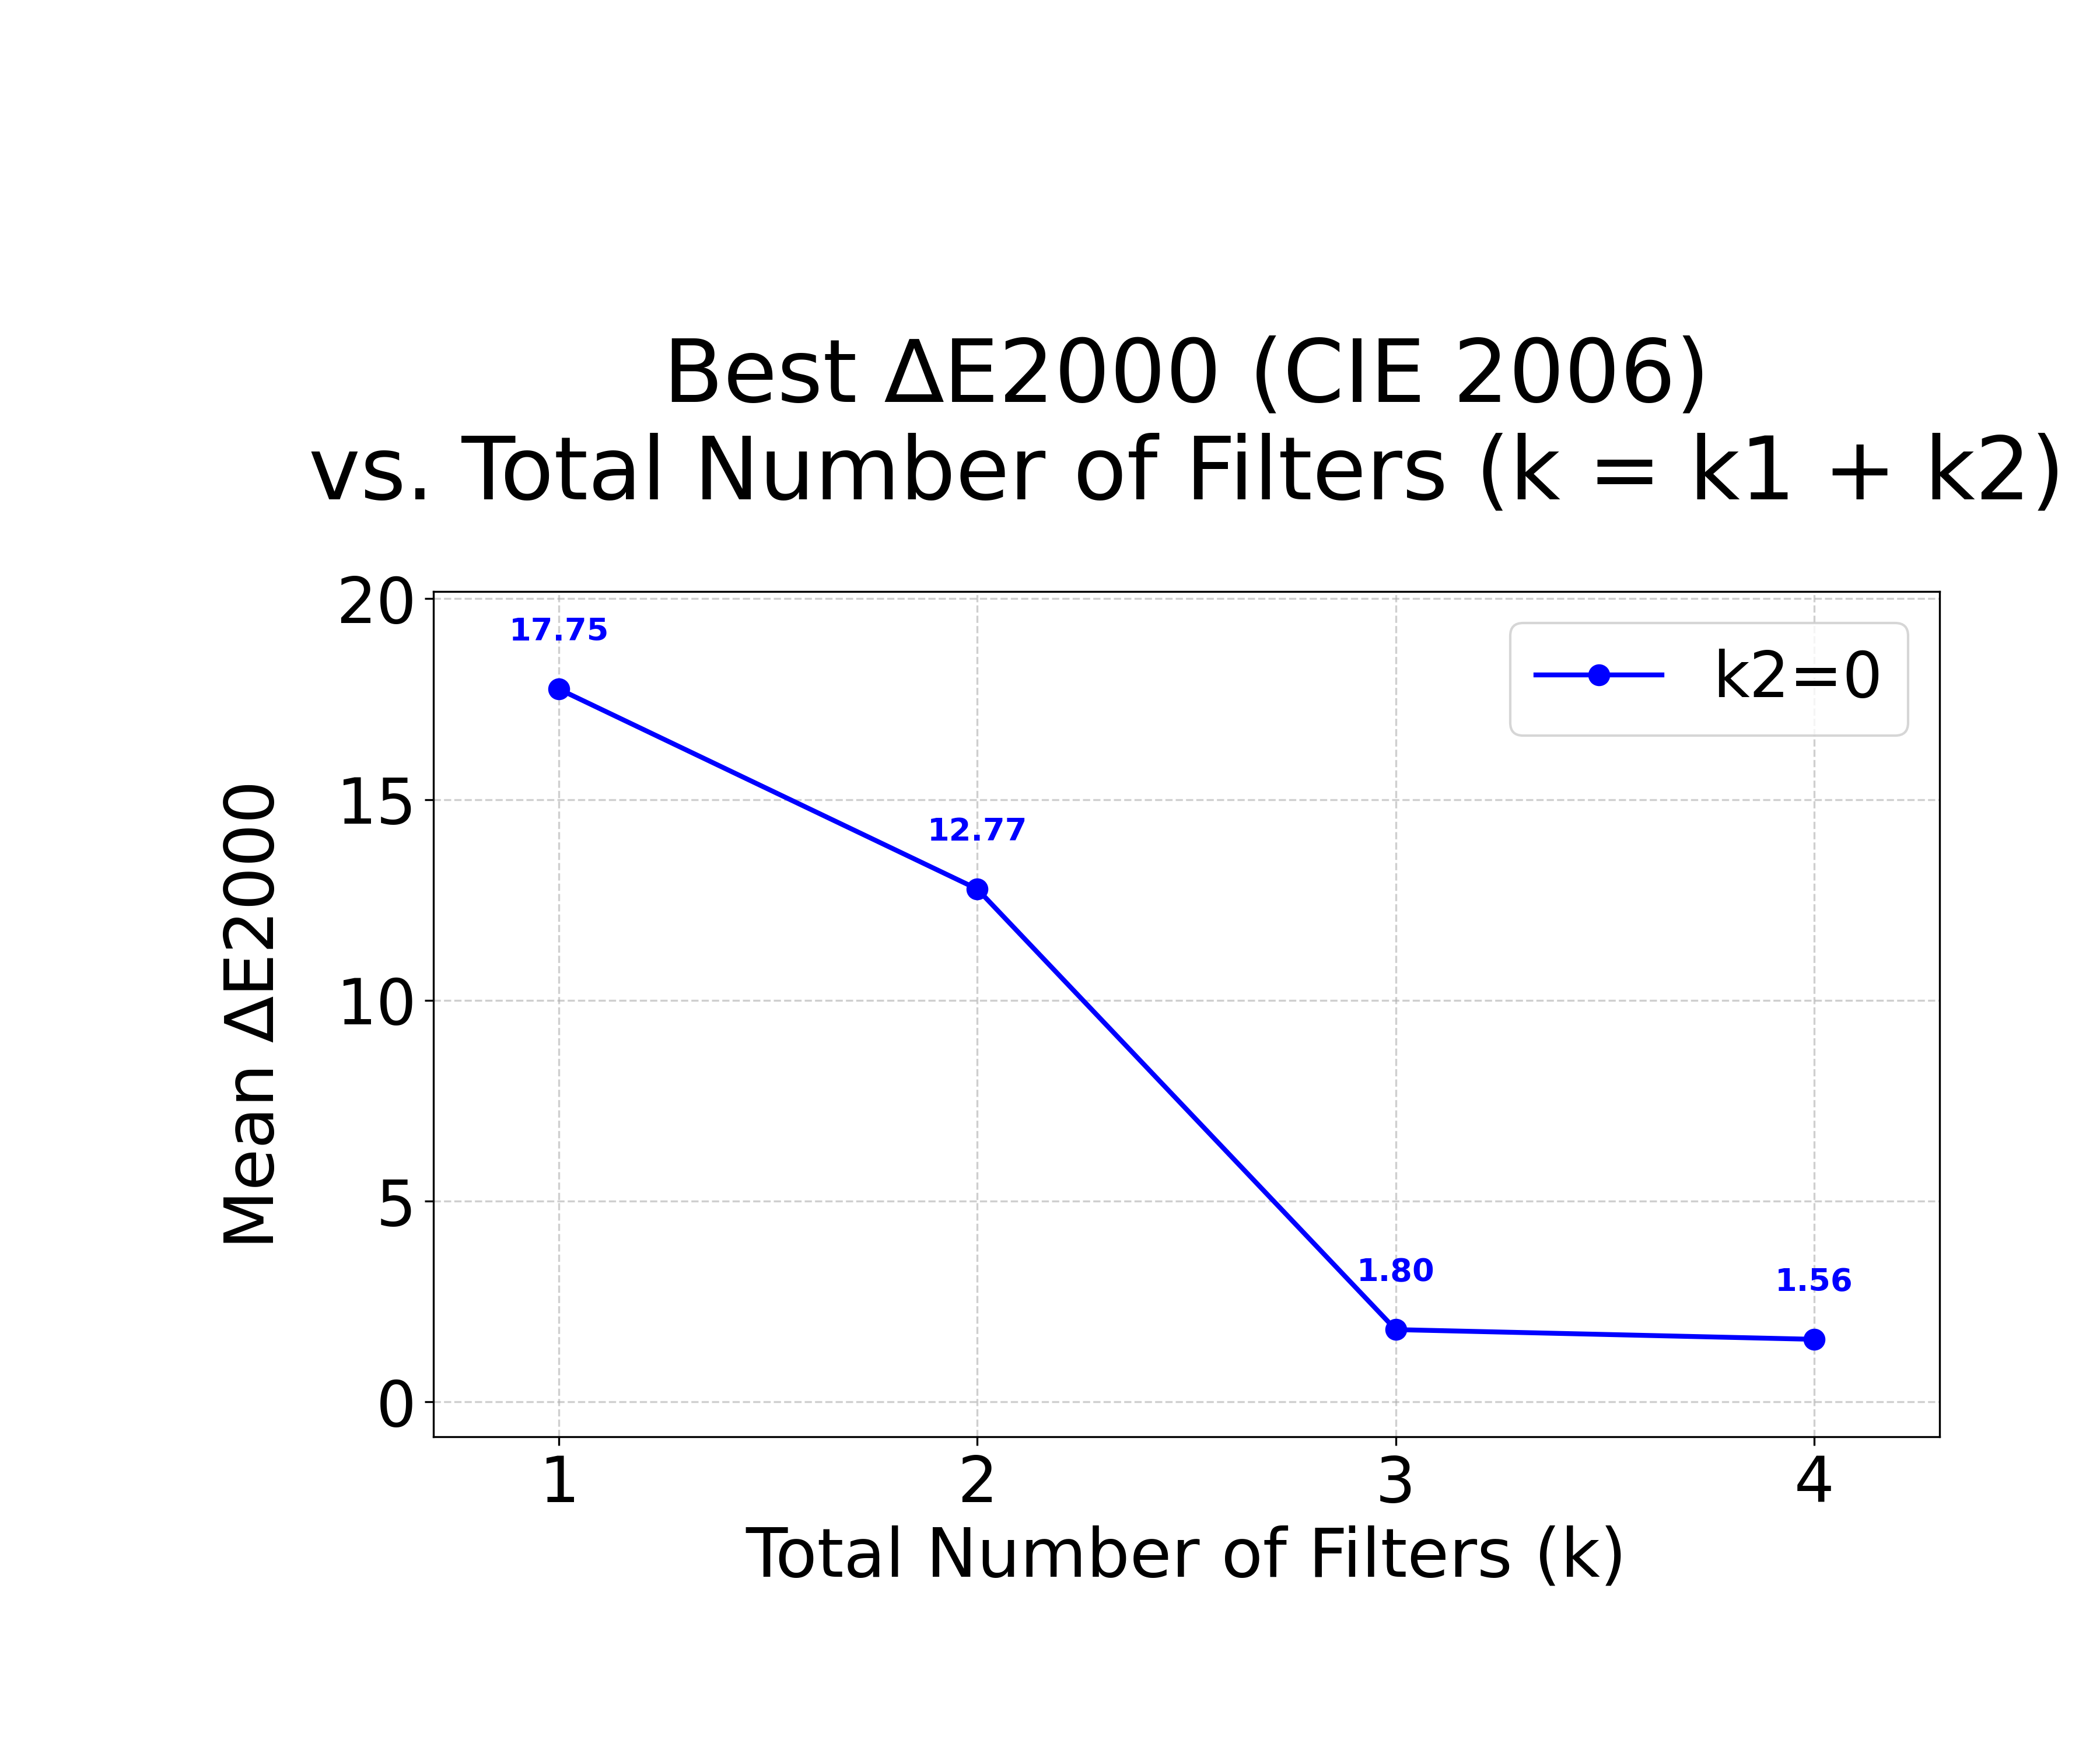
\includegraphics[width=\linewidth]{media/scraped_k4_nDeltaEChart.png}
    \caption{Mean $\dE$ of best combination for each number of scraped filters $k < 5$}
\end{subfigure}%
\begin{subfigure}{.49\linewidth}
    \centering
    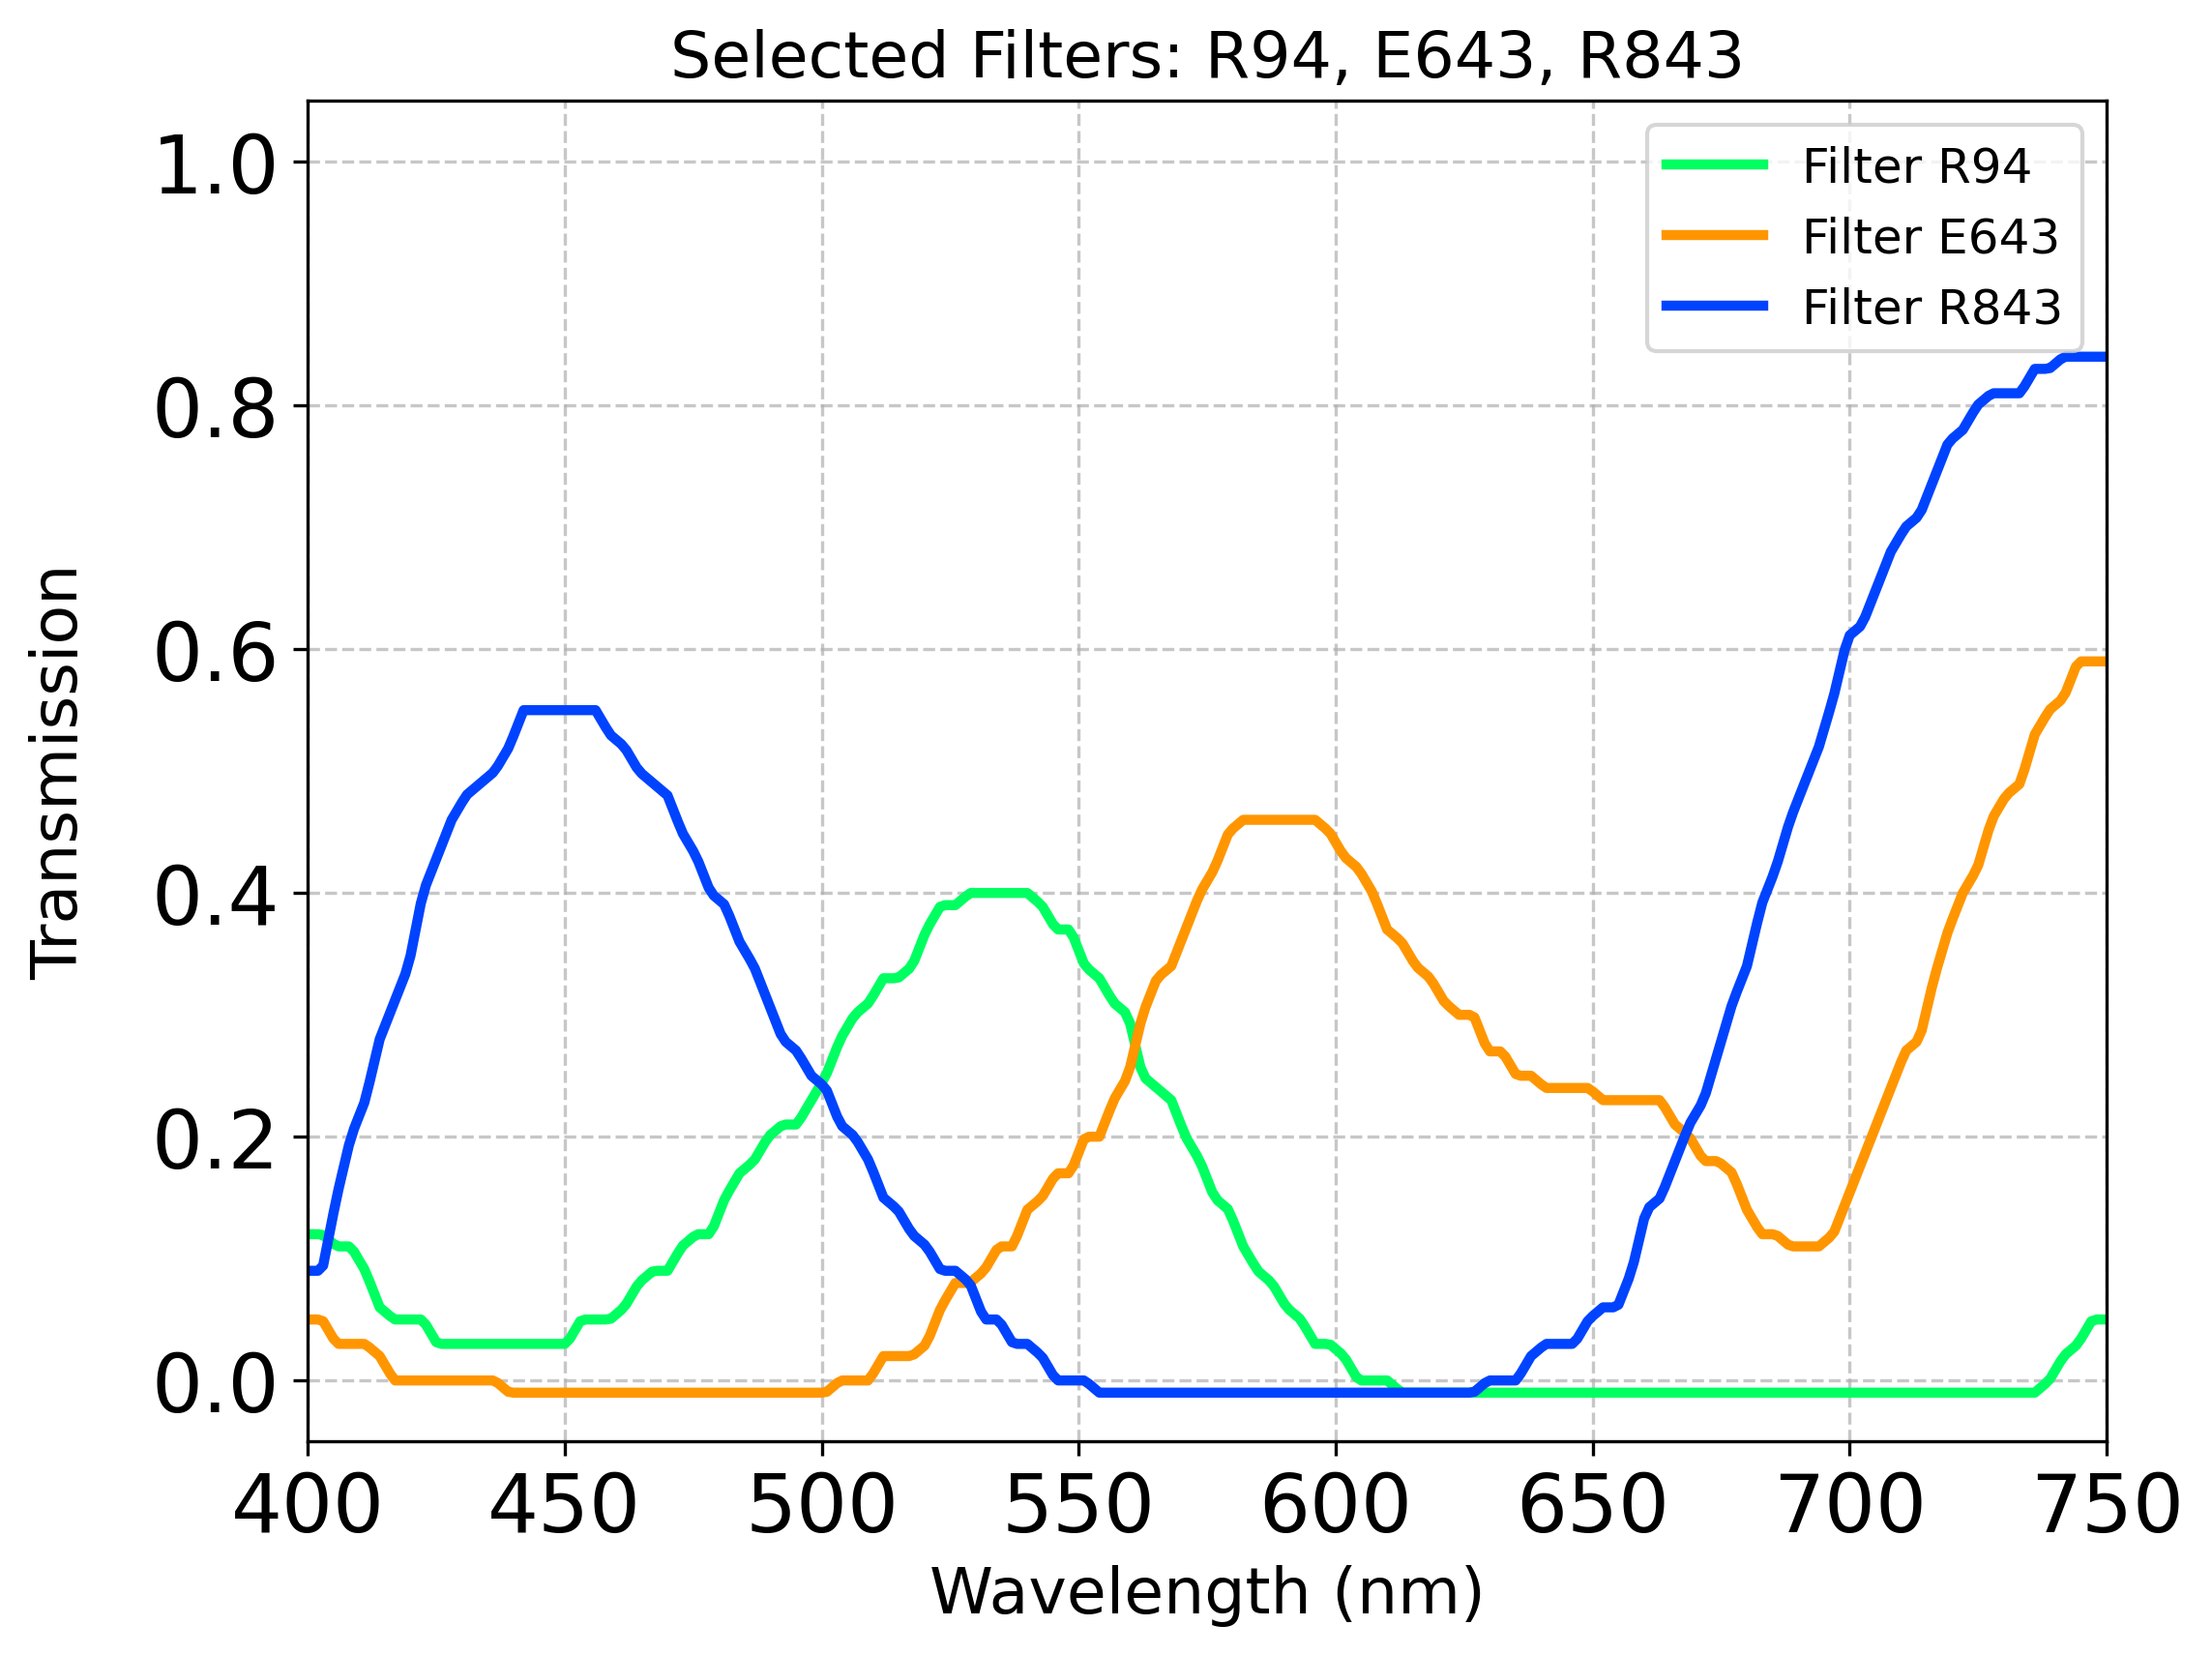
\includegraphics[width=\linewidth]{media/scraped_k3_front_page_right.png}
    \caption{Transmission functions for optimal MyColor $k=3$ solution}
\end{subfigure}
\caption{MyColor $k<5$ performance and selected filters.}
\end{figure}

Indeed, we can visually inspect the transmission functions above to see that our functions share approximate modes with the XYZ functions, given that the right tails will be neutralized above 650nm by the presence of our IR-cut filter.

Their transformations after multiplication by $\boldsymbol{M}$ are shown below, including a simulated IR-cut filter which cuts off most transmission above 650nm.
These are overlaid on the CIE 2006 XYZ (from LMS) functions.

\begin{figure}[H]
\centering
\begin{subfigure}{.55\linewidth}
    \centering
    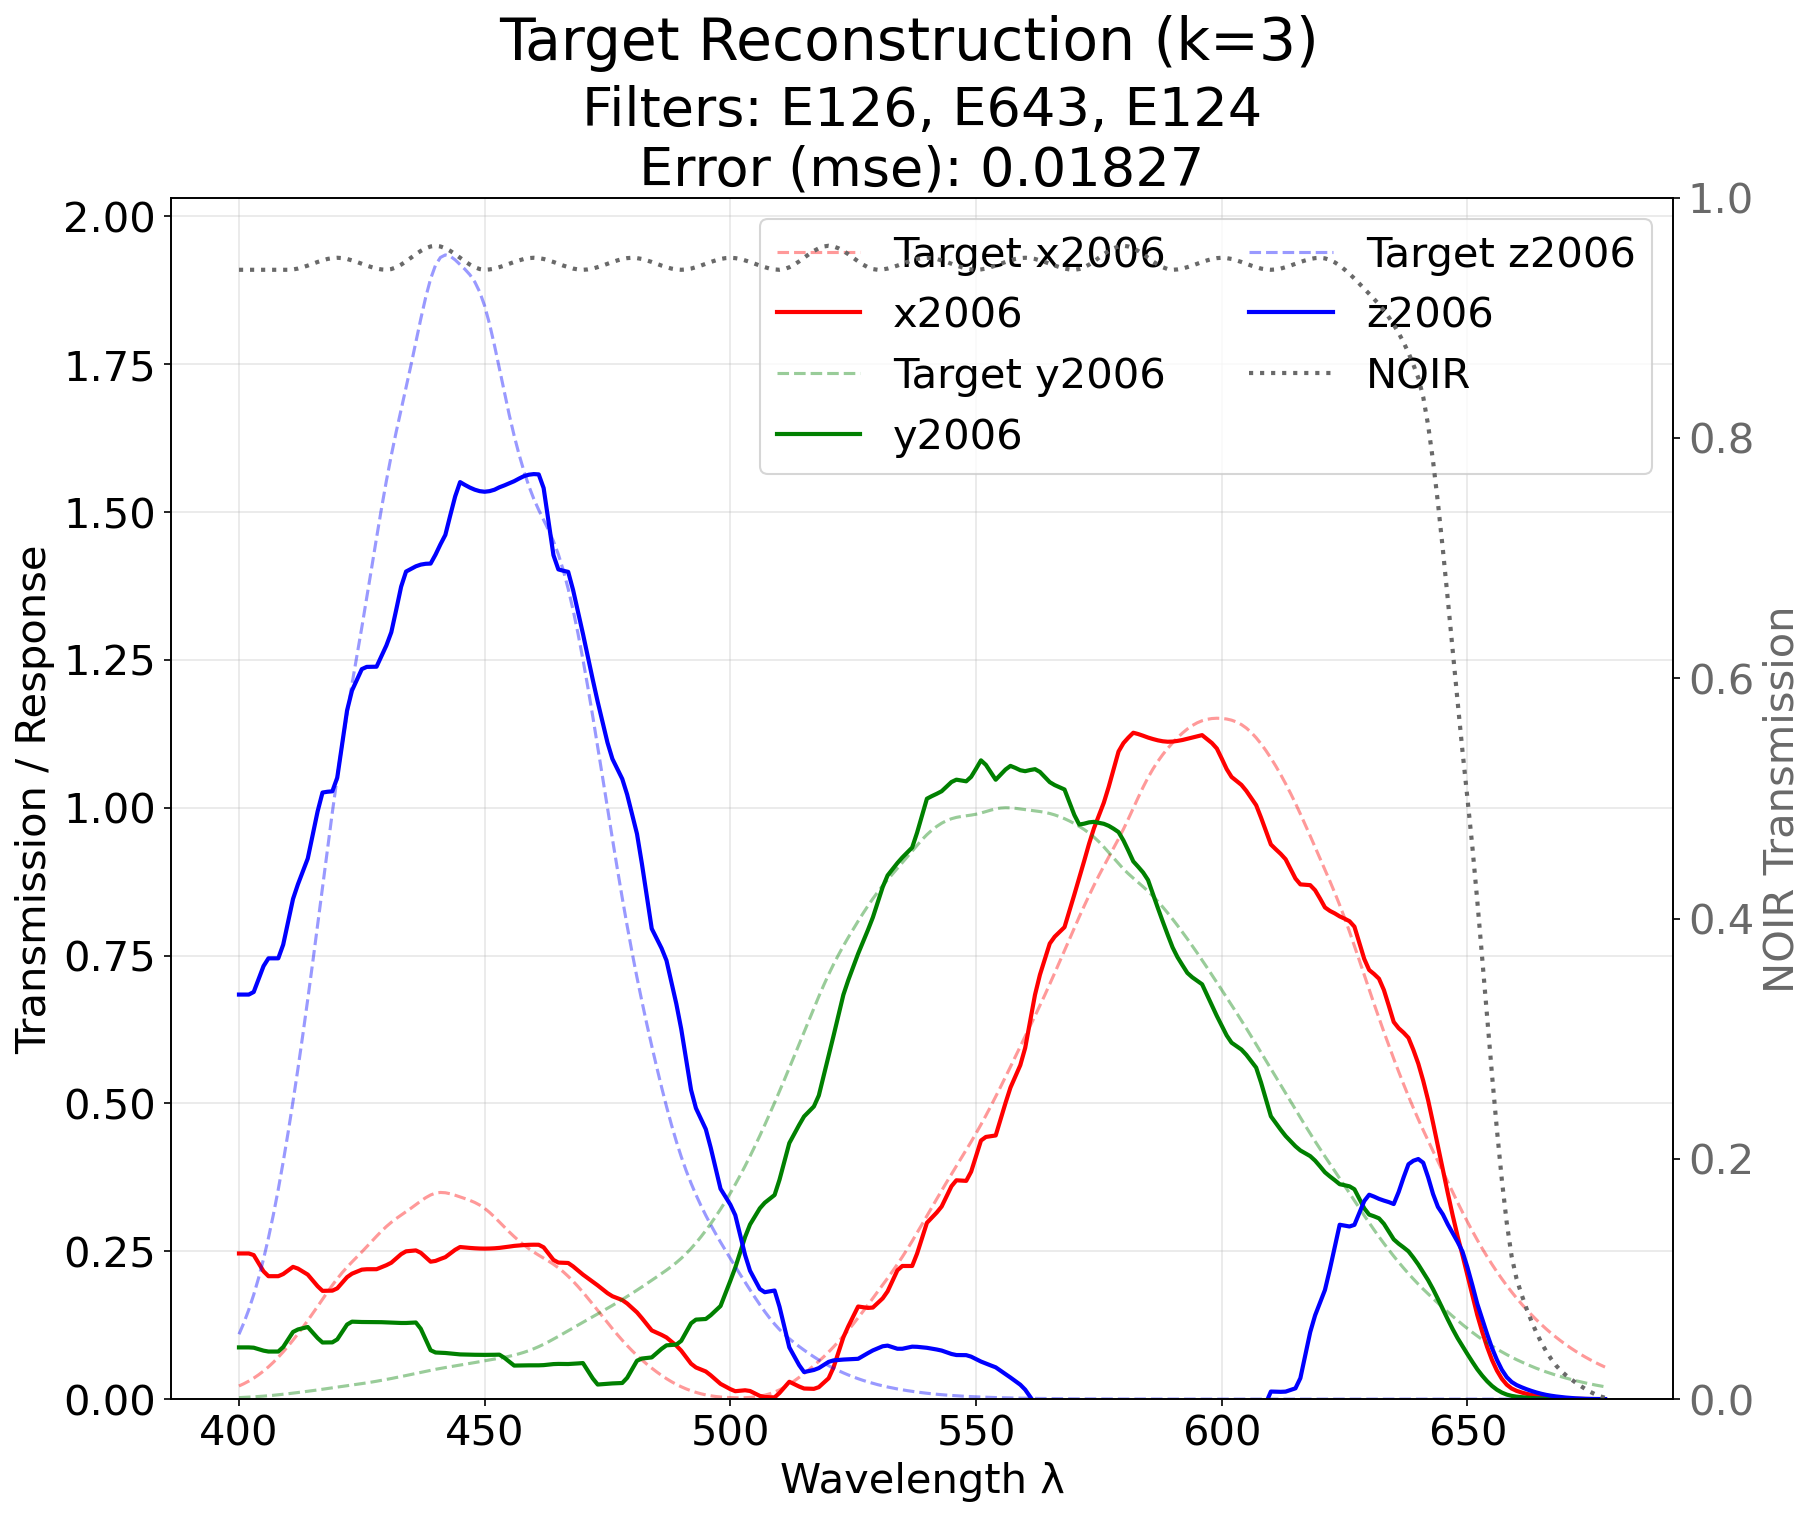
\includegraphics[width=\linewidth]{media/scraped_k3_spectra.png}
    \caption{Transformed transmission functions with CIE 2006 XYZ spectral response functions}
\end{subfigure}%
\begin{subfigure}{.44\linewidth}
    \centering
    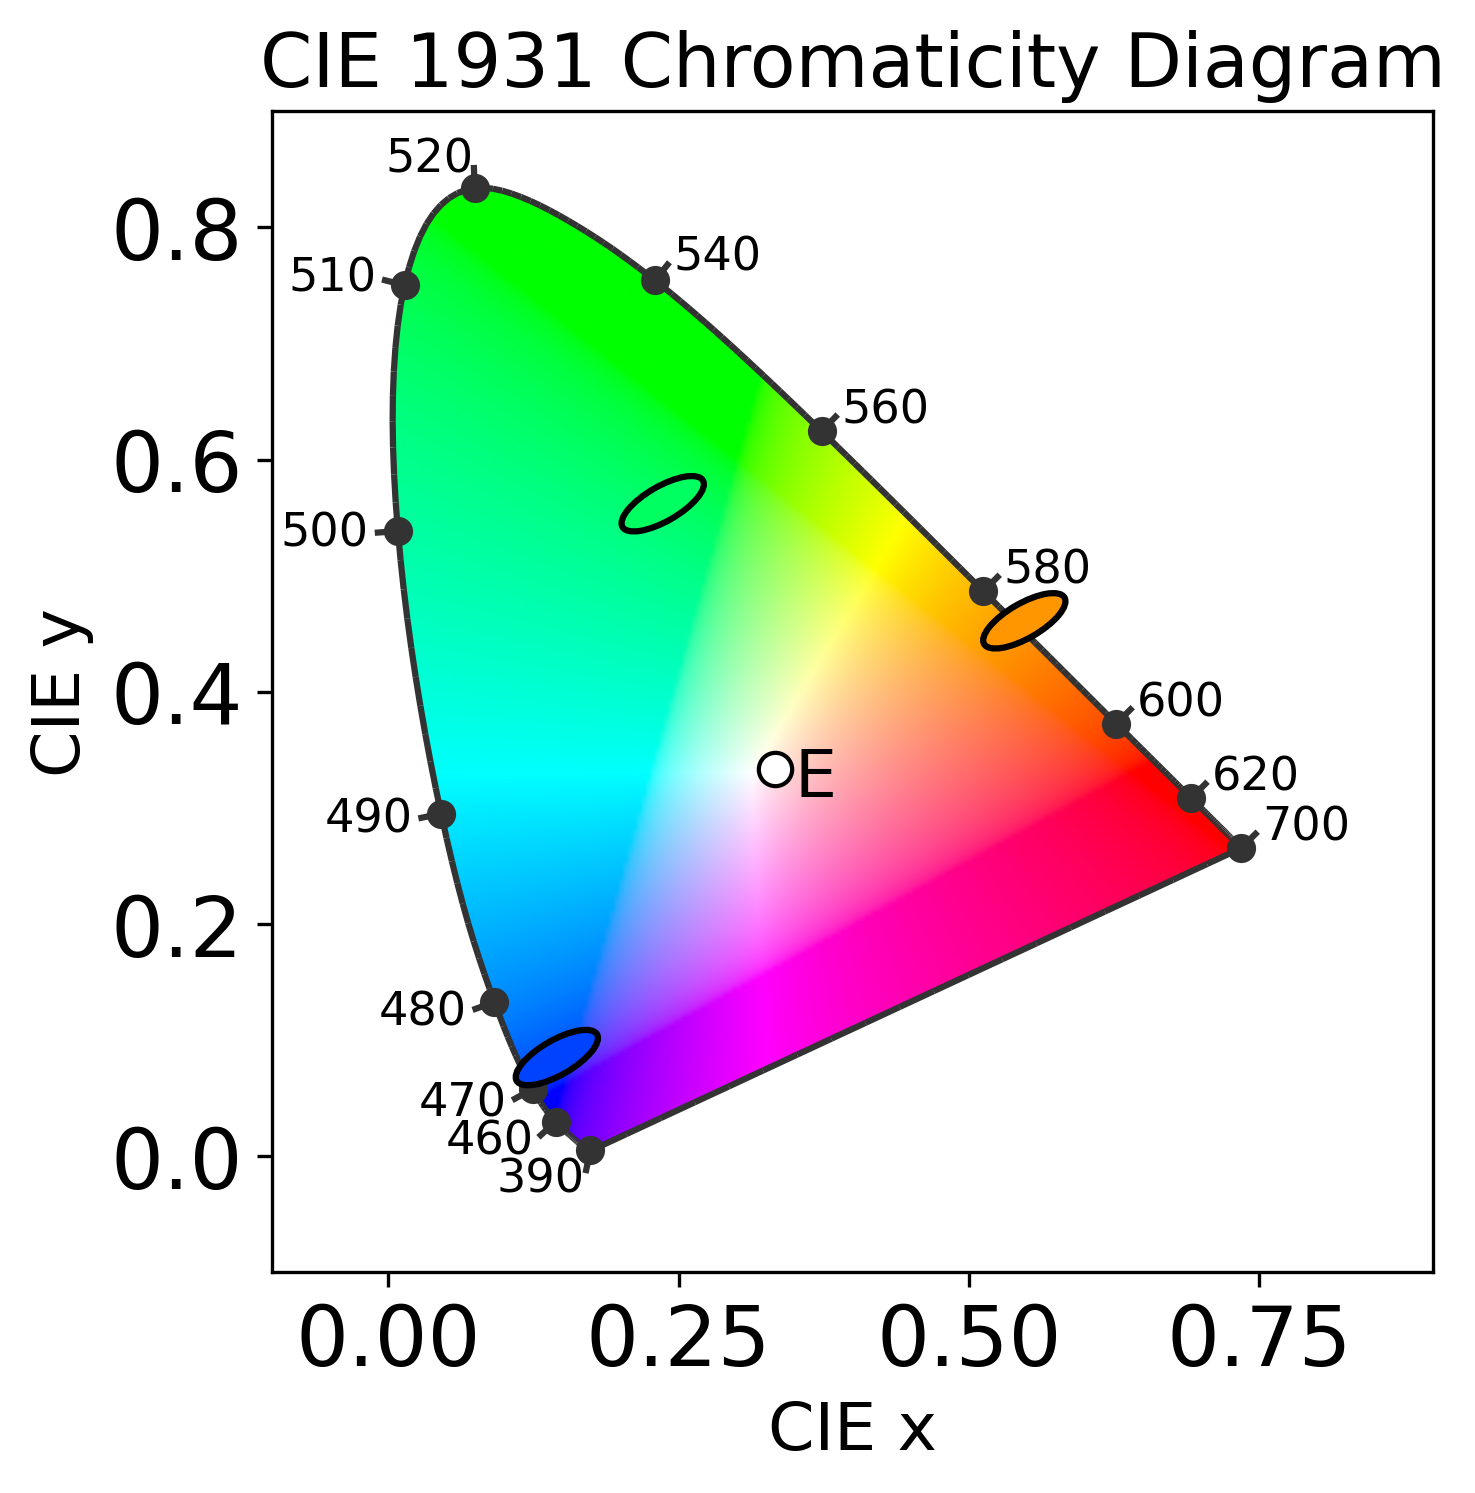
\includegraphics[width=\linewidth]{media/scraped_gamut_k3.png}
    \caption{Best filters from MyColor at $k=3$ on the color gamut}
\end{subfigure}
\caption{MyColor $k=3$ filters in spectral and chromaticity space.}
\end{figure}

Additionally, we can view the filters' dominant wavelength overlaid onto the CIE 1931 Chromaticity Diagram in CIE x and CIE y space to see that these filters 'span' the entire gamut, and hence a linear combination of these filters may effectively reproduce any color on the gamut.
While we primarily utilize the New CIE 2006 LMS functions and their respective XYZ transformations (denoted CIE 2006), a significant body of research exists referring to the 1931 XYZ functions which provide helpful benchmarks for our performance. 
Further, the CIE 1931 Color Gamut diagram provides a natural and familiar demonstration of color within the CIE x and CIE y coordinates.  

More rigorous analysis requires the use of $\dE$ calculations using a color checker, and in this case, our mean $\dE$ across 24 patches reached the value of 1.80.

\begin{figure}[H]
\centering
\begin{subfigure}{.4\linewidth}
    \centering
    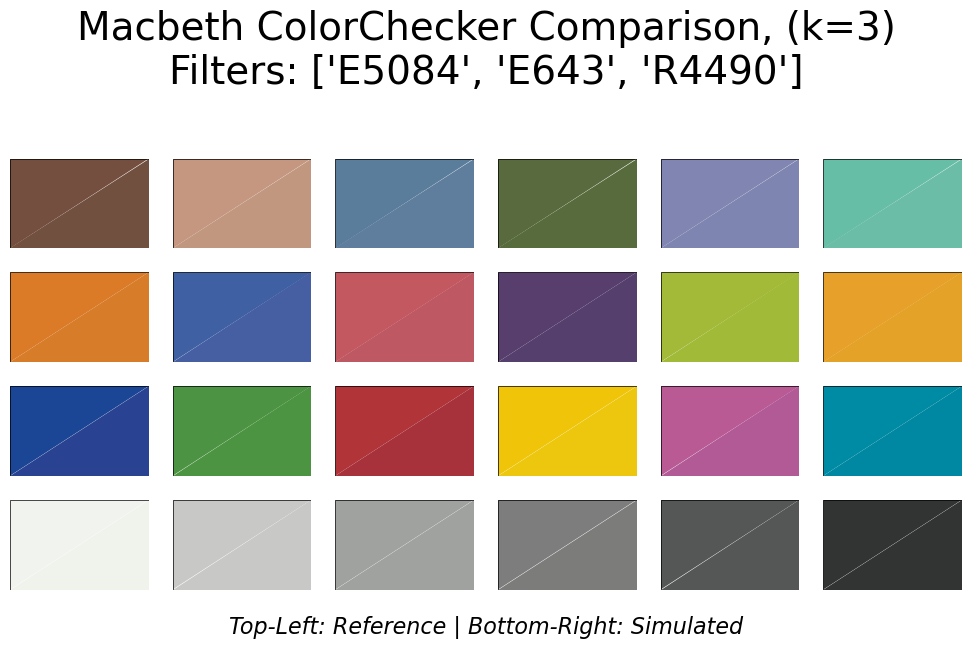
\includegraphics[width=\linewidth]{media/scraped_k3_macbeth.png}
    \caption{Macbeth Color Checker for $k=3$ with MyColor filters}
\end{subfigure}%
\begin{subfigure}{.45\linewidth}
    \centering
    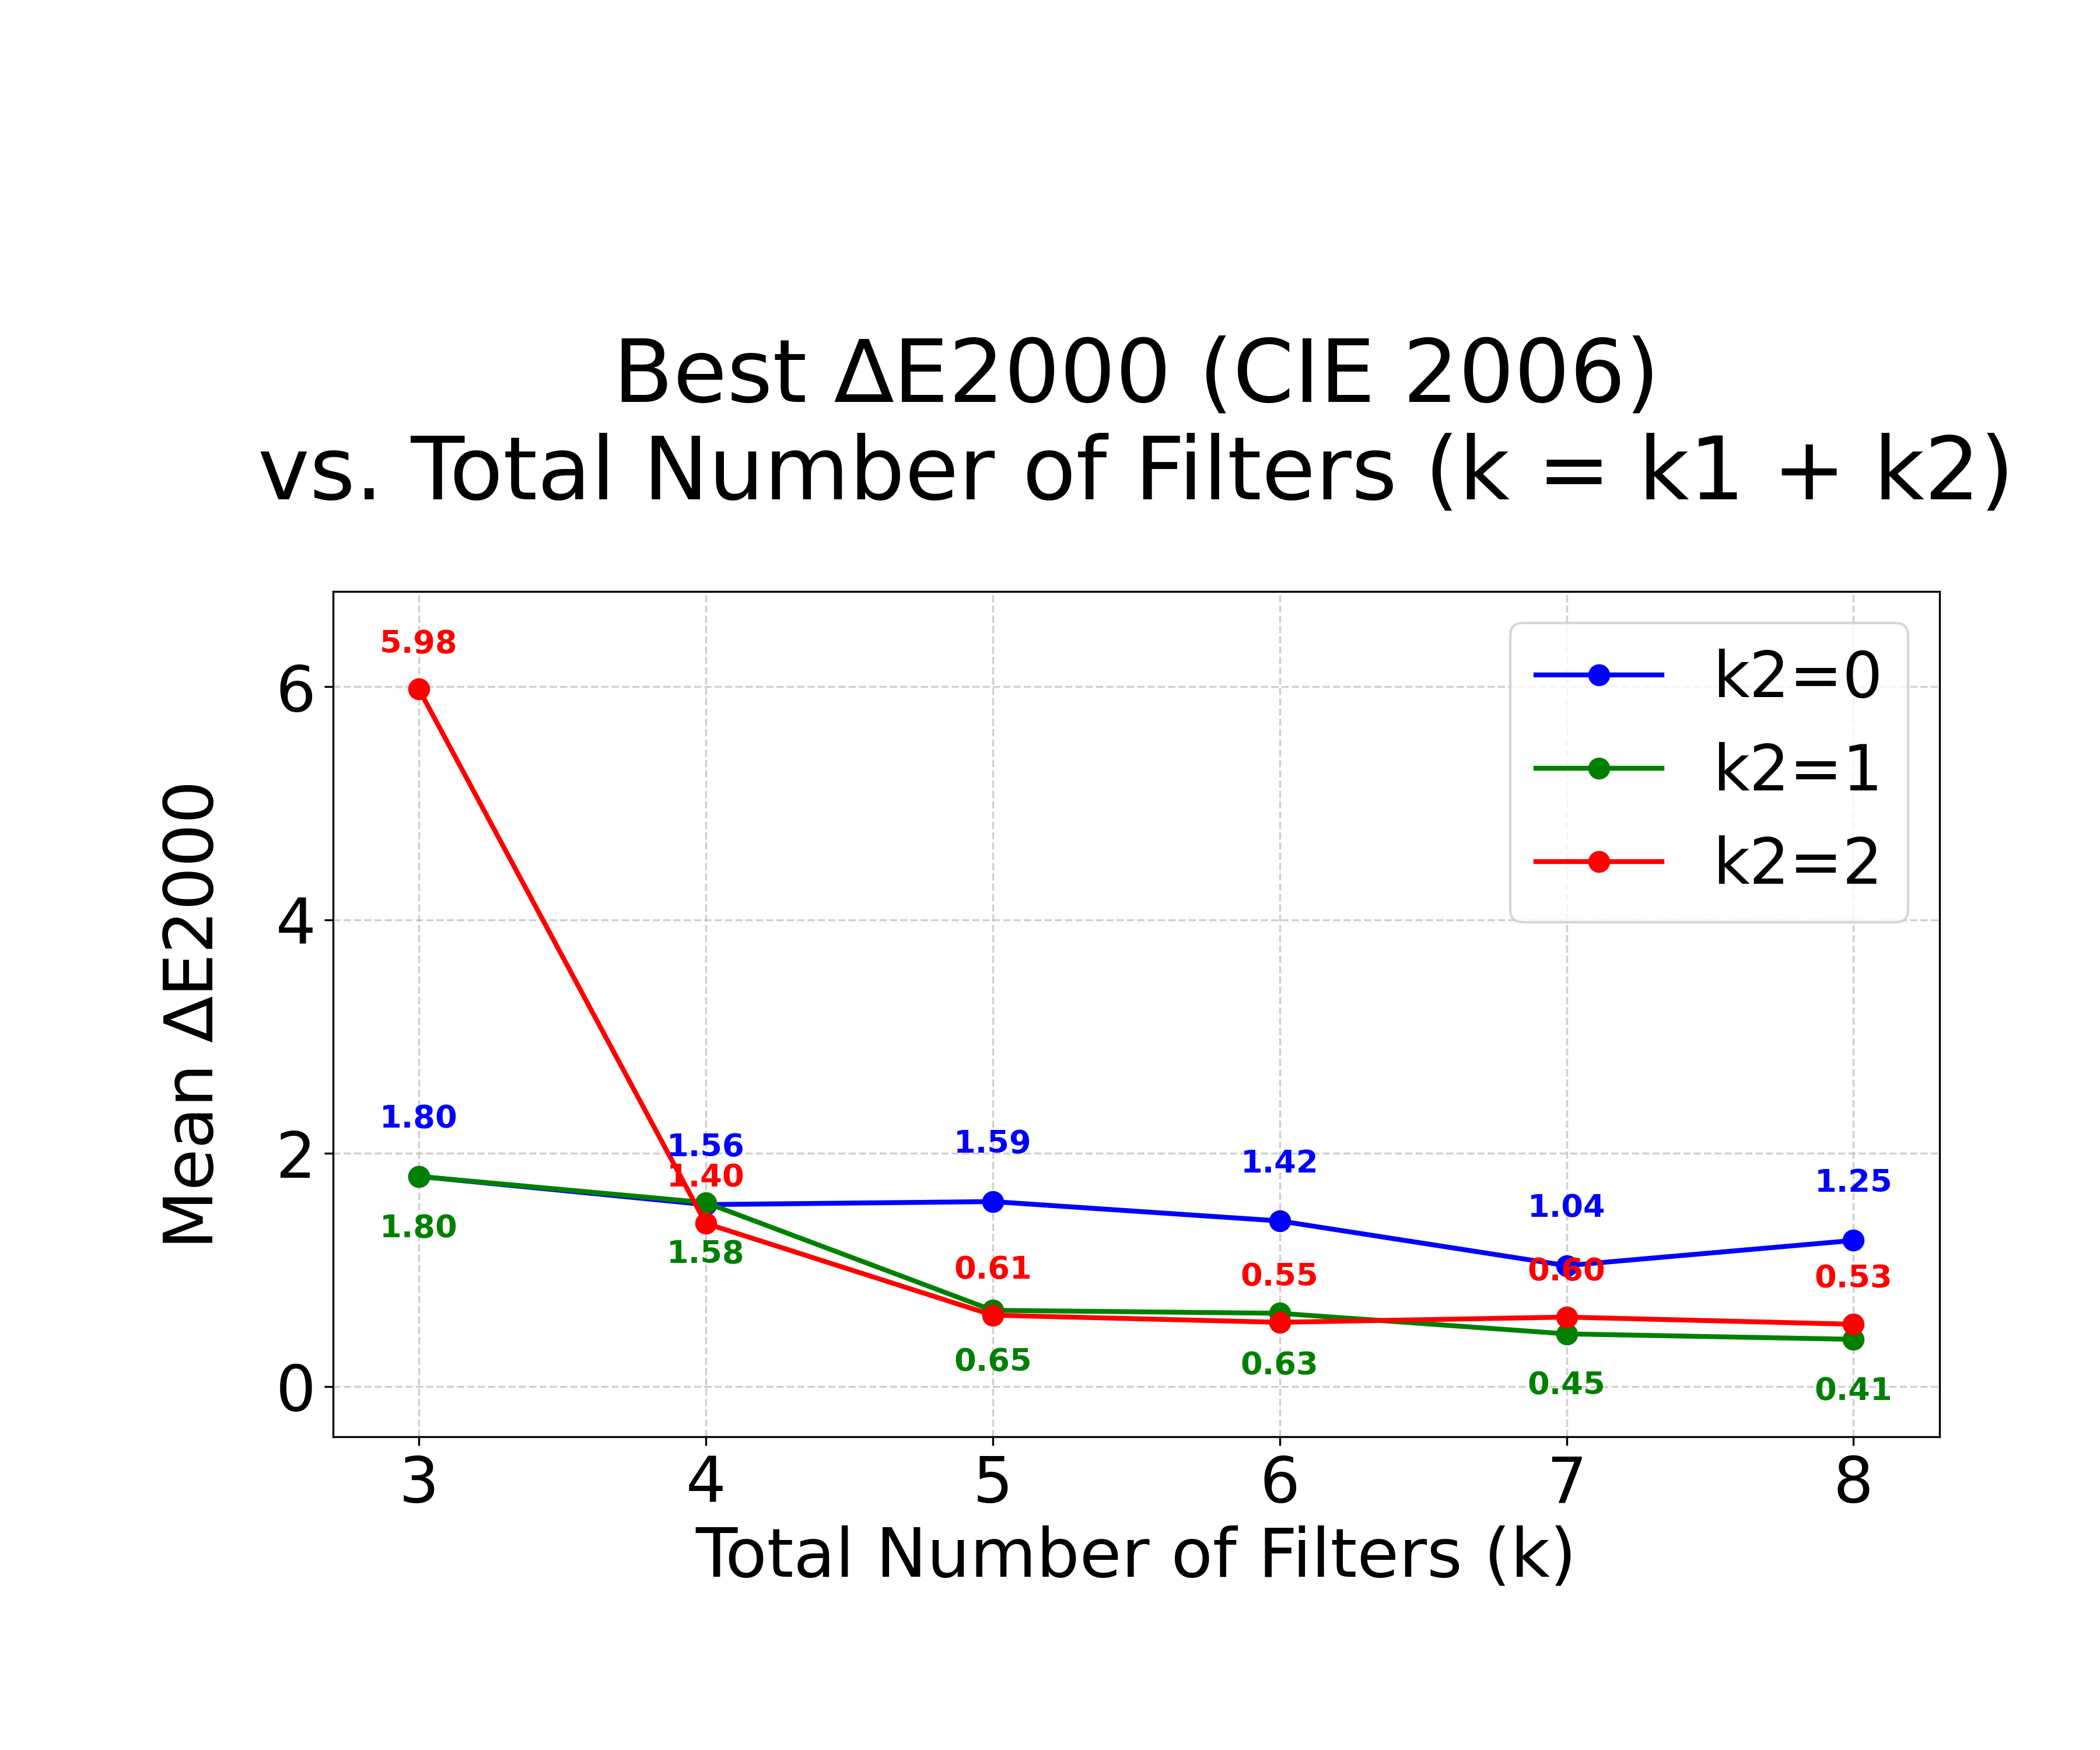
\includegraphics[width=\linewidth]{media/scraped_k1scaled_deltaE.png}
    \caption{$\dE$ for $k \in \{3...8\}$ and $k_1 \in \{0,1,2\}$}
\end{subfigure}
\caption{MyColor evaluation on a color checker and scaling to larger $k$.}
\end{figure}

While $\dE$ of 1.80 is sufficient for human-centered applications in controlled lighting, we can improve upon this result and strive for lower MSE results.
With the full set of 494 filters, we are unable to compute a brute-force solution in reasonable time, and must utilize heuristic solutions.
Fortunately, the heuristic solutions augmented with a few brute force rounds provide effective solutions. 
We show up to $k=8$ filters' $\dE$ progressions as a function of $k$ above. 

This result supports our intuition that we can achieve $\dE$ values comparable with state of the art results using our analysis.
Importantly, the improvement in $\dE$ largely flattens after $k=5$, providing useful knowledge as to the necessary number of filters to attain a high-quality reconstruction.
We include a rendering from the CAVE dataset reconstructed with the $k=5 (k_1=4,k_2=1)$ solution for an example of a practical simulated filter wheel setup. 
We also provide the $k=2 (k_1=2,k_2=0), \dE=12.77$ solution for comparison.  

\begin{figure}[H]
\centering
\begin{subfigure}{.49\linewidth}
    \centering
    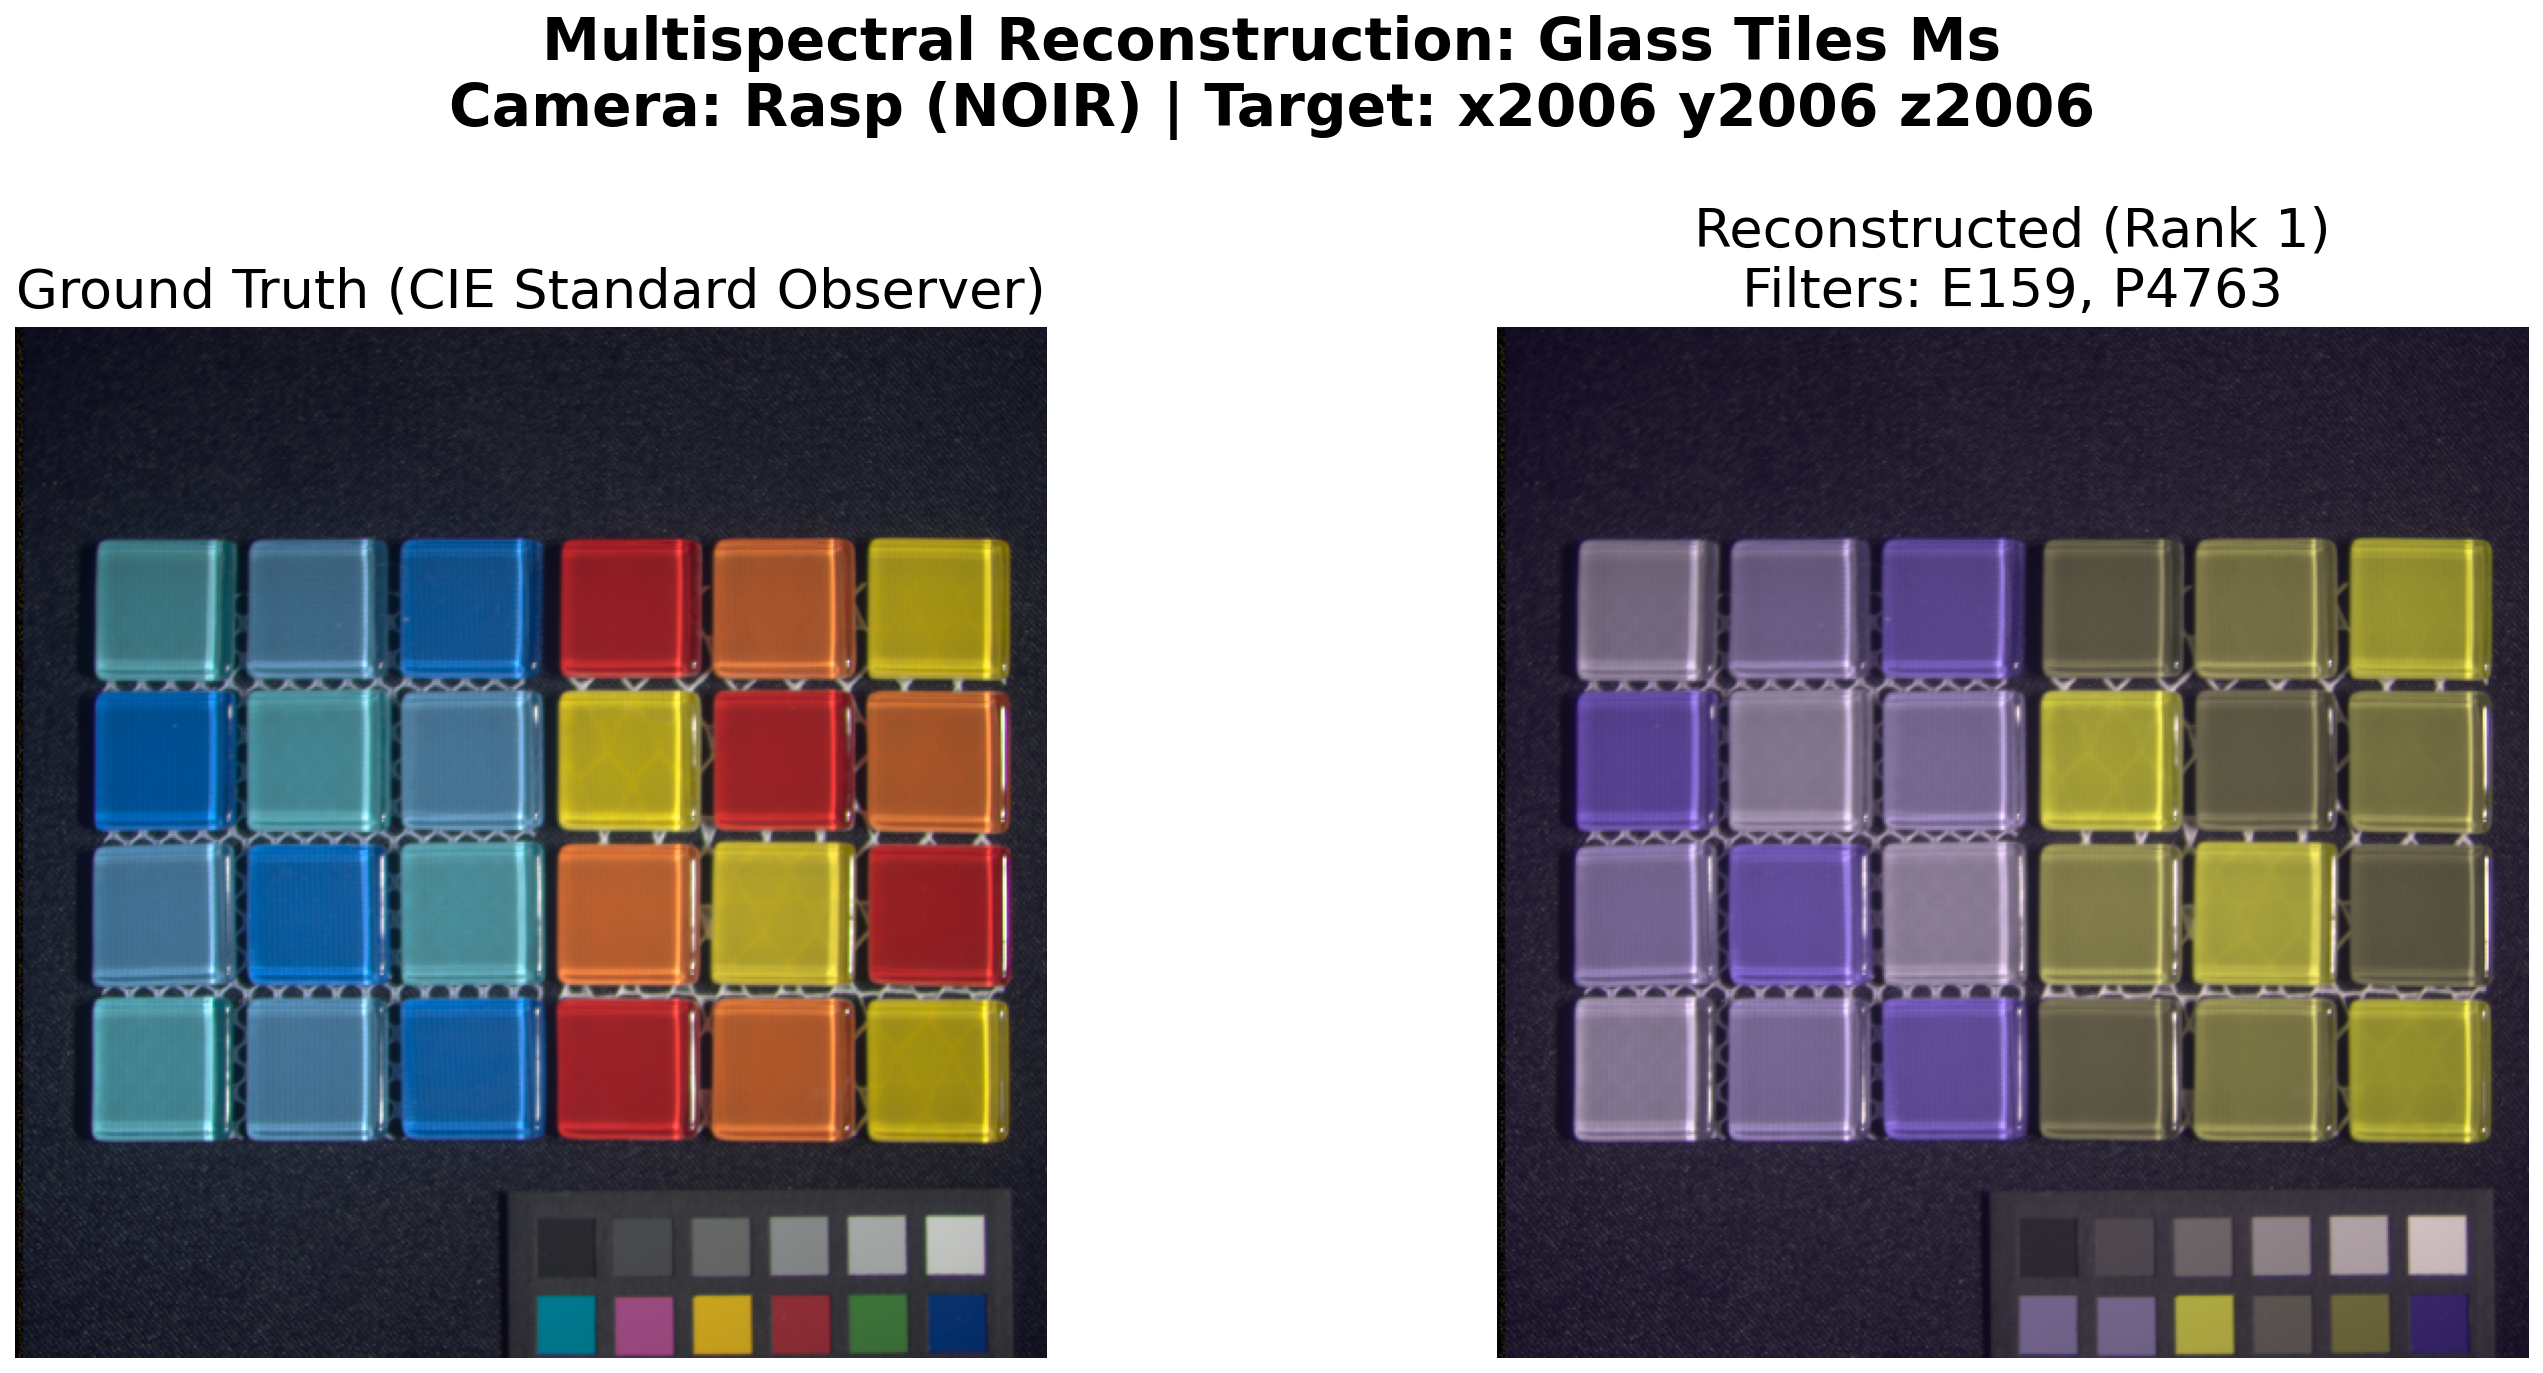
\includegraphics[width=\linewidth]{media/scraped_tiles_cave_k2.png}
    \caption{CAVE 'glass tiles' scene with scraped filters, $k=2 (k_1=2,k_2=0)$}
\end{subfigure}%
\begin{subfigure}{.49\linewidth}
    \centering
    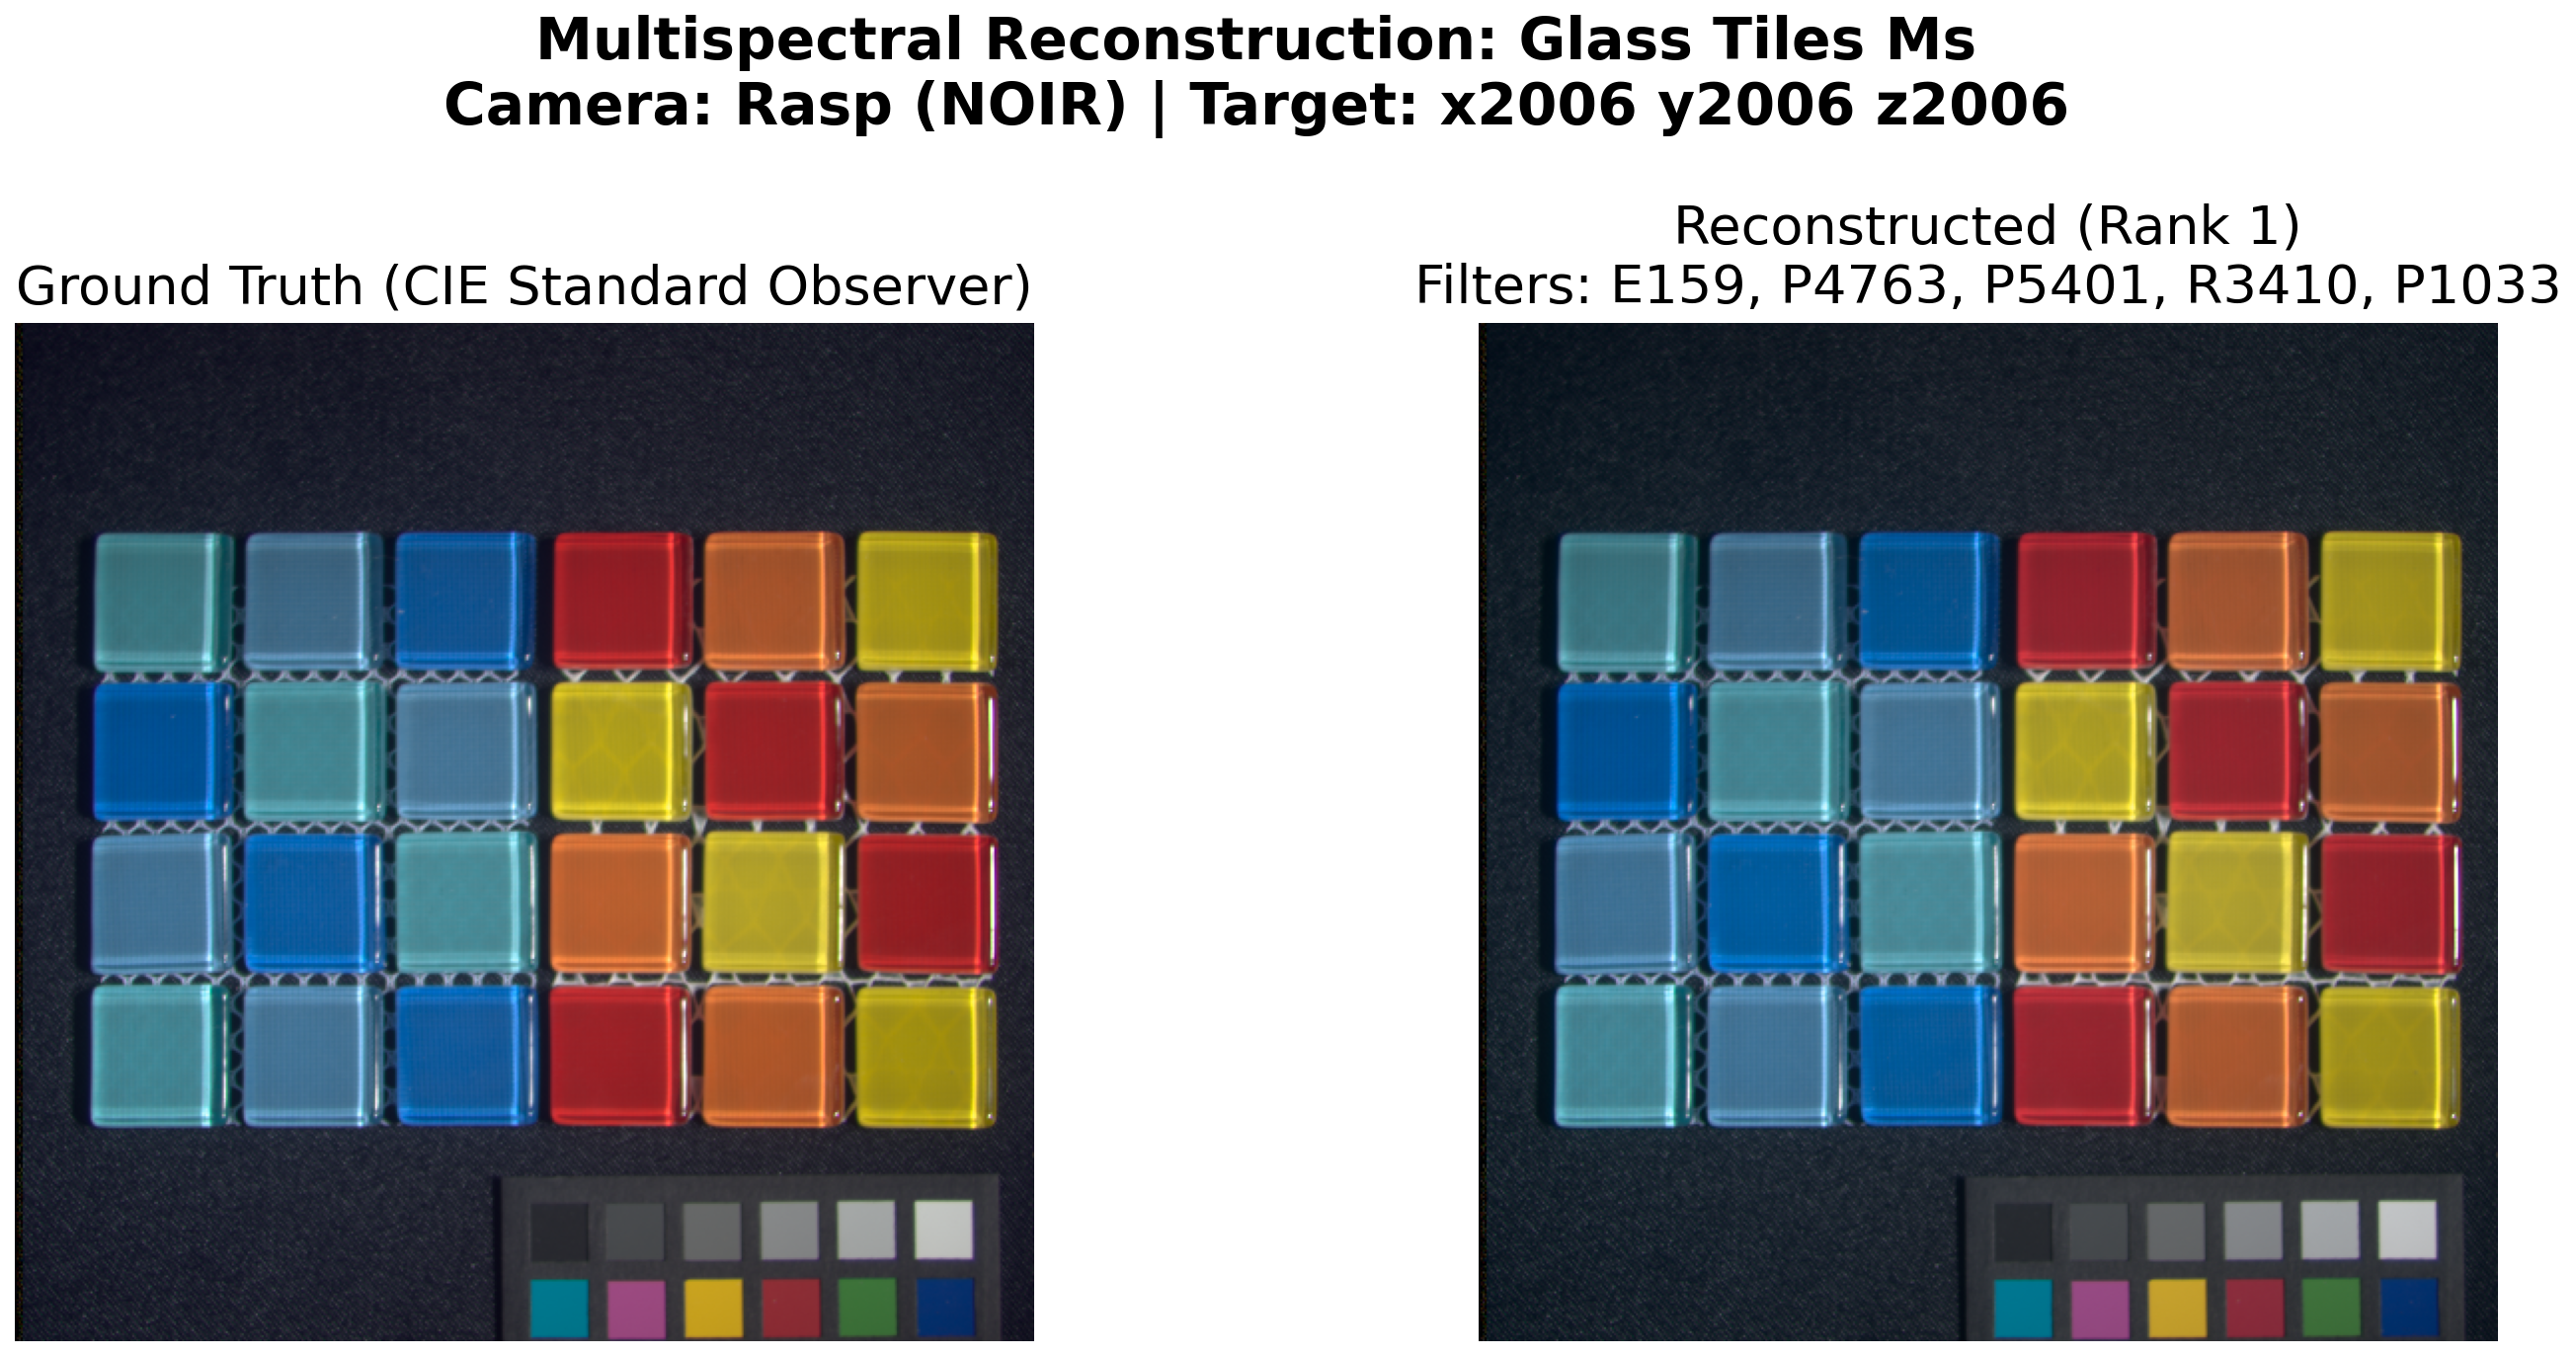
\includegraphics[width=\linewidth]{media/scraped_tiles_cave_k5.png}
    \caption{CAVE 'glass tiles' scene with scraped filters $k=5 (k_1=4,k_2=1)$}
\end{subfigure}
\caption{Comparison of different CAVE renders with scraped filters}
\end{figure}

We note that the set of 494 filters provides a large candidate pool, making it comparatively easy to reconstruct the desired target functions, subject to our ability to correctly identify a good combination. 
In the next section, we explore a similar analysis on a smaller set of filters, searching for an equivalent reconstruction quality and more easily calculating the performance difference against the best possible solution as found by brute force, which we cannot feasibly compute for the $N=494$ sized set of filters. 

\section{Rosco Supergel Set in Simulated Camera}

In this section, we progressively increase the number of filters $k$ and analyze the reconstruction quality for each. 
We comment on the increases in reconstruction quality afforded by each incremental extra capture, understanding that each filter increases capture time and possibility of a 'bad capture.'
Specifically, because  we require a mechanical servo turn between each capture, if an object in our scene moves, or worse, if our camera moves during capture, our reconstruction will be irrecoverably damaged. 

To maintain consistency across this demonstration, we run all the simulations in the following section with an IR-cut filter included. 
Additionally, for the computations of $\dE$, we utilize the python \codeword{color} and \codeword{colour-science} libraries, with the CIE 1931 or 2015 2 Degree Standard Observer respectively, depending on whether we utilize the CIE 1931 or CIE 2006 XYZ functions. 
D65 illuminant from the same library is used as well as ColorChecker N Ohta reflectance patches. XYZ responses were converted to CIELAB using the \codeword{color.xyz2lab} function to convert XYZ signals to lab before $\dE$ computation.

\subsection{MSE, $\dE$ and CAVE Results for $k \in \{3,4,5\}$}

We will provide some filter wheel prescriptions along the various values of $k$ we consider for our filter wheel. 
In Figure \ref{fig:supergelIntro}, we show the best $\dE$ of our approximation at each $k$ filter subset of the Rosco Supergel set, where $k\in \{1,8\}$. 
For completeness and surety of optimal combination identification, we use brute force search in this section, thus $k=k_1$ and we omit $k_2$.
In this section, we continue to use the IR-cut filter and a standard MSE loss for consistency versus the prior section and other works. 

\begin{figure}[H]
\centering
\begin{subfigure}{.46\linewidth}
    \centering
    \includegraphics[width=\linewidth]{media/deltaE_vs_k_mse.png}
    \caption{Best $\dE$ for each number of filters $k$}
\end{subfigure}
\begin{subfigure}{.53\linewidth}
    \centering
    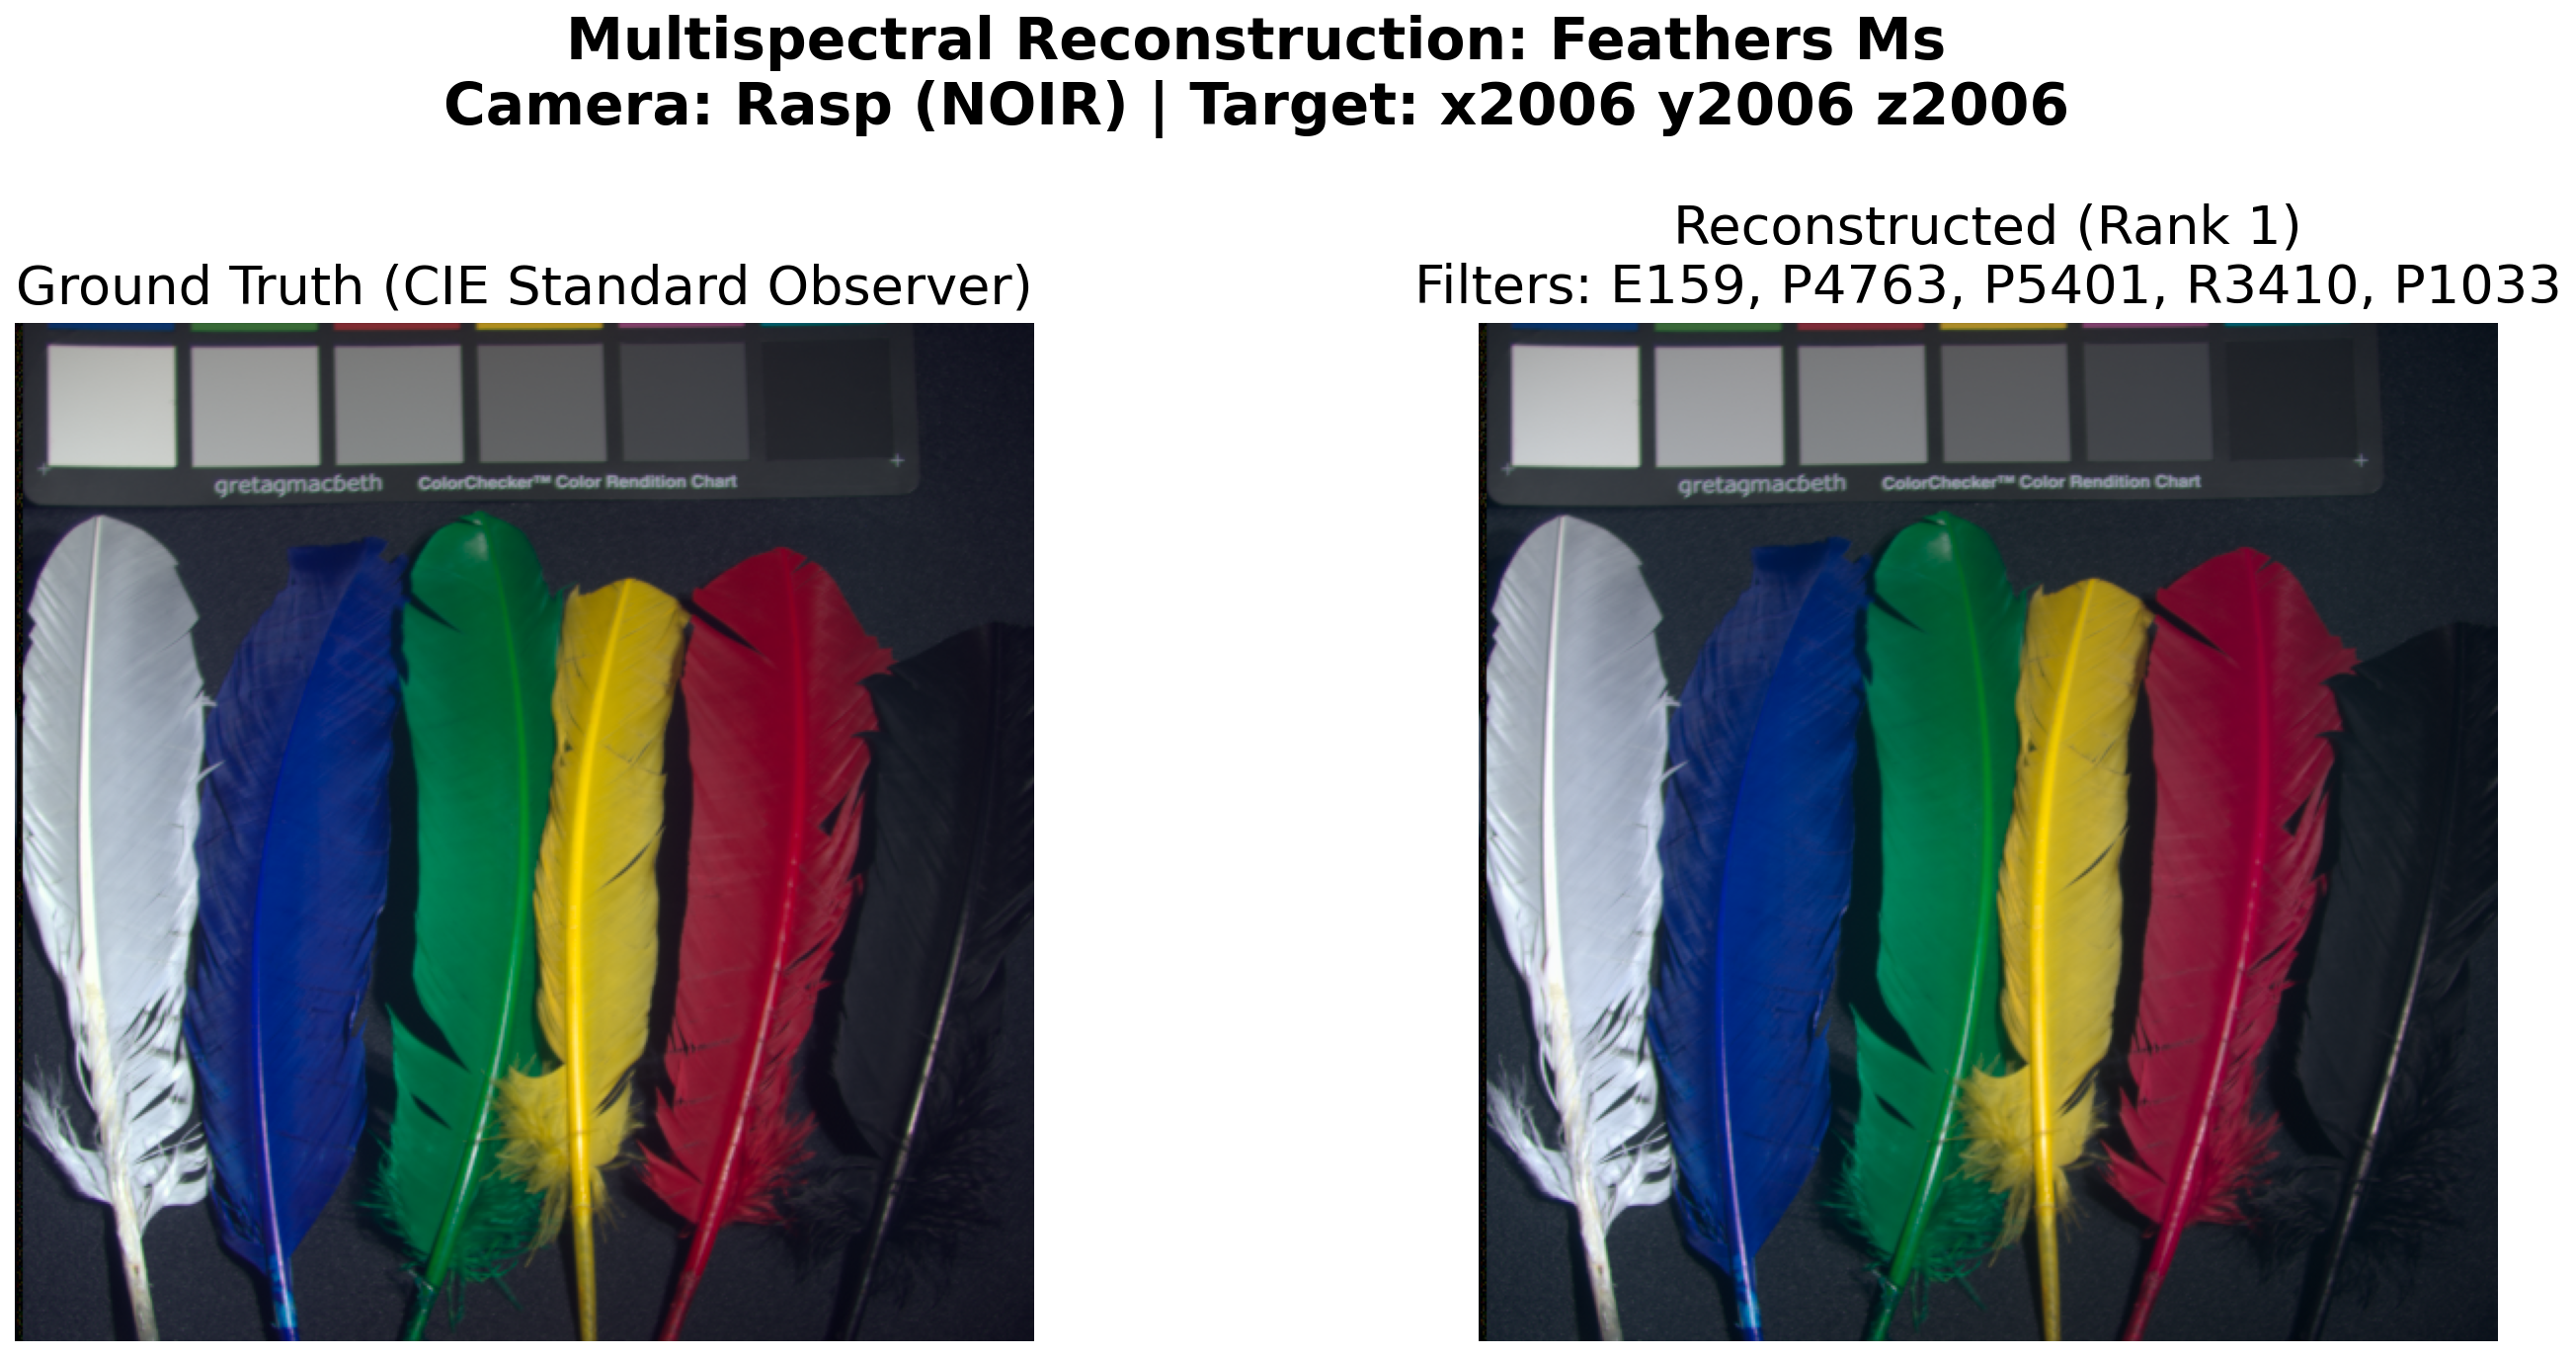
\includegraphics[width=\linewidth]{media/scraped_cave.png}
    \caption{CAVE rendering using best $k=5$ solution}
\end{subfigure}%
\caption{Example simulated reconstruction and overall Supergel set performance.}
\label{fig:supergelIntro}
\end{figure}

\subsubsection{Solution for $k=3$}

The best filter combination for $k=3$, clearly a poor spectral fit, see Fig. \ref{fig:k3spectral}, achieves a tolerable mean $\dE$ of 3.77. This is in the just noticeable difference threshold of 2-4 \cite{lindstrom2008delta},
indicating that the reconstructed colors may be distinguishable from the target colors under certain conditions. 
The 24 patches above show the original in the top left of each pane and the simulated reconstruction in the bottom right. It is evident there is a visible colour difference.
\begin{figure}[H]
\centering
\begin{subfigure}{.49\linewidth}
    \centering
    \includegraphics[width=\linewidth]{media/k3top1_spectra.png}
    \caption{Best XYZ reconstruction}
\end{subfigure}%
\begin{subfigure}{.49\linewidth}
    \centering
    \includegraphics[width=\linewidth]{media/n3MSEMacbeth.png}
    \caption{Macbeth Color Checker comparison}
\end{subfigure}
\begin{subfigure}{.49\linewidth}
    \centering
    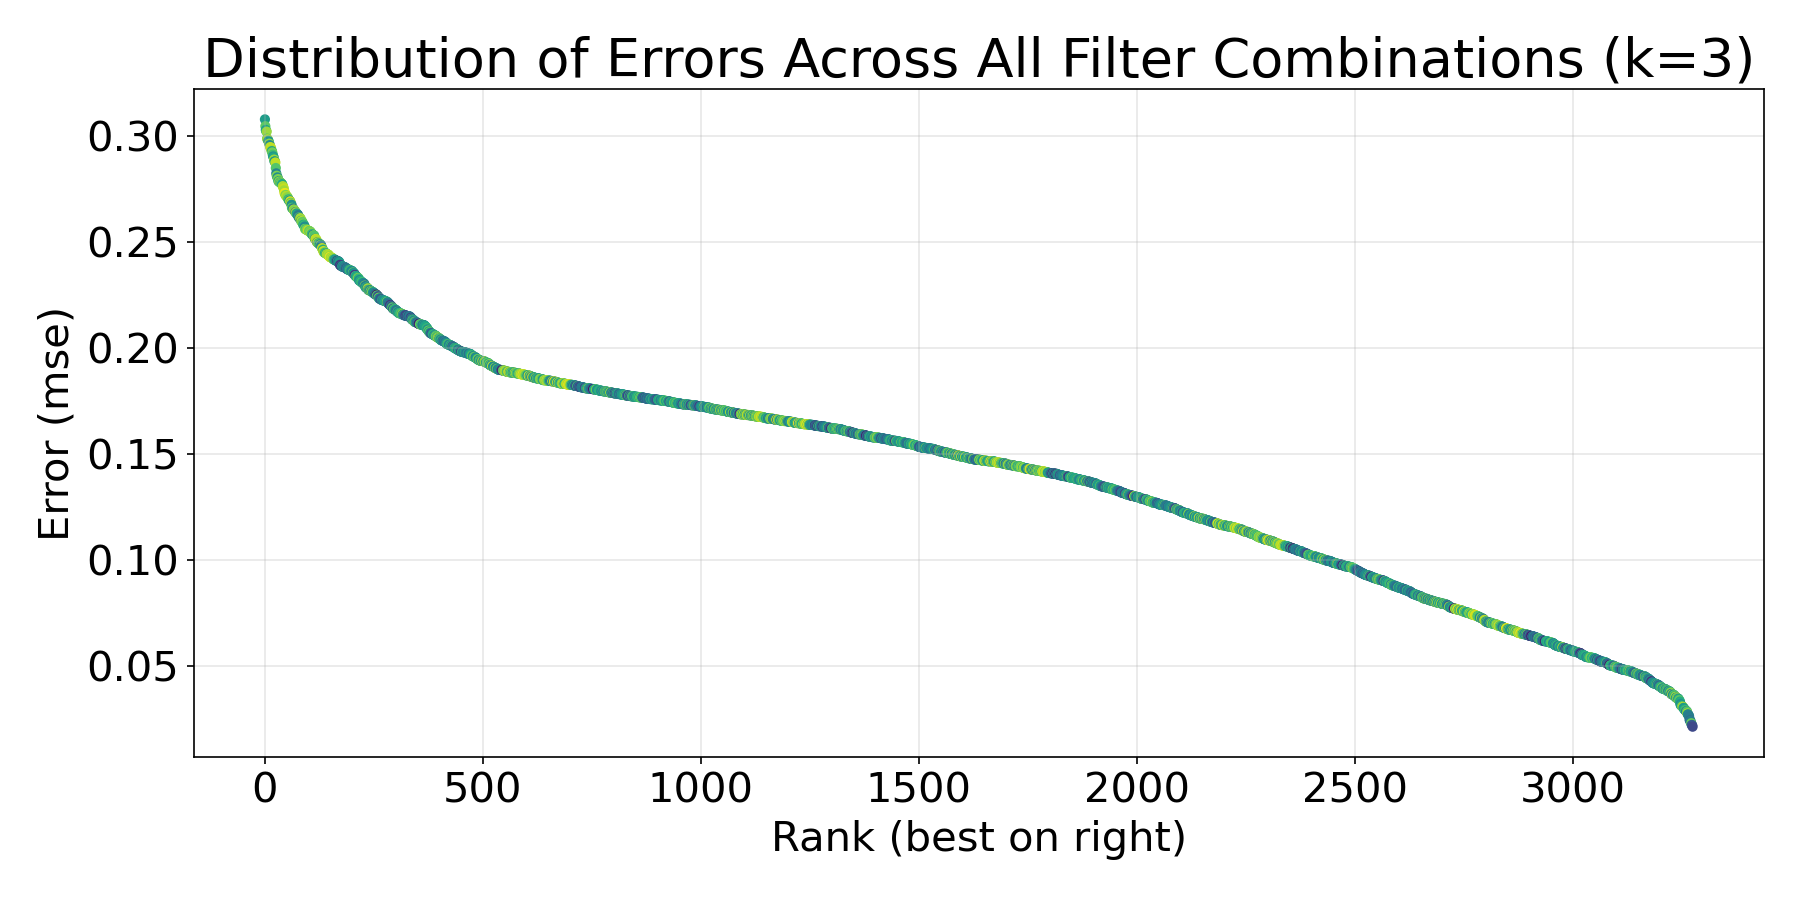
\includegraphics[width=\linewidth]{media/measured_k3_errors.png}
    \caption{Error distribution across combinations}
\end{subfigure}%
\begin{subfigure}{.49\linewidth}
    \centering
    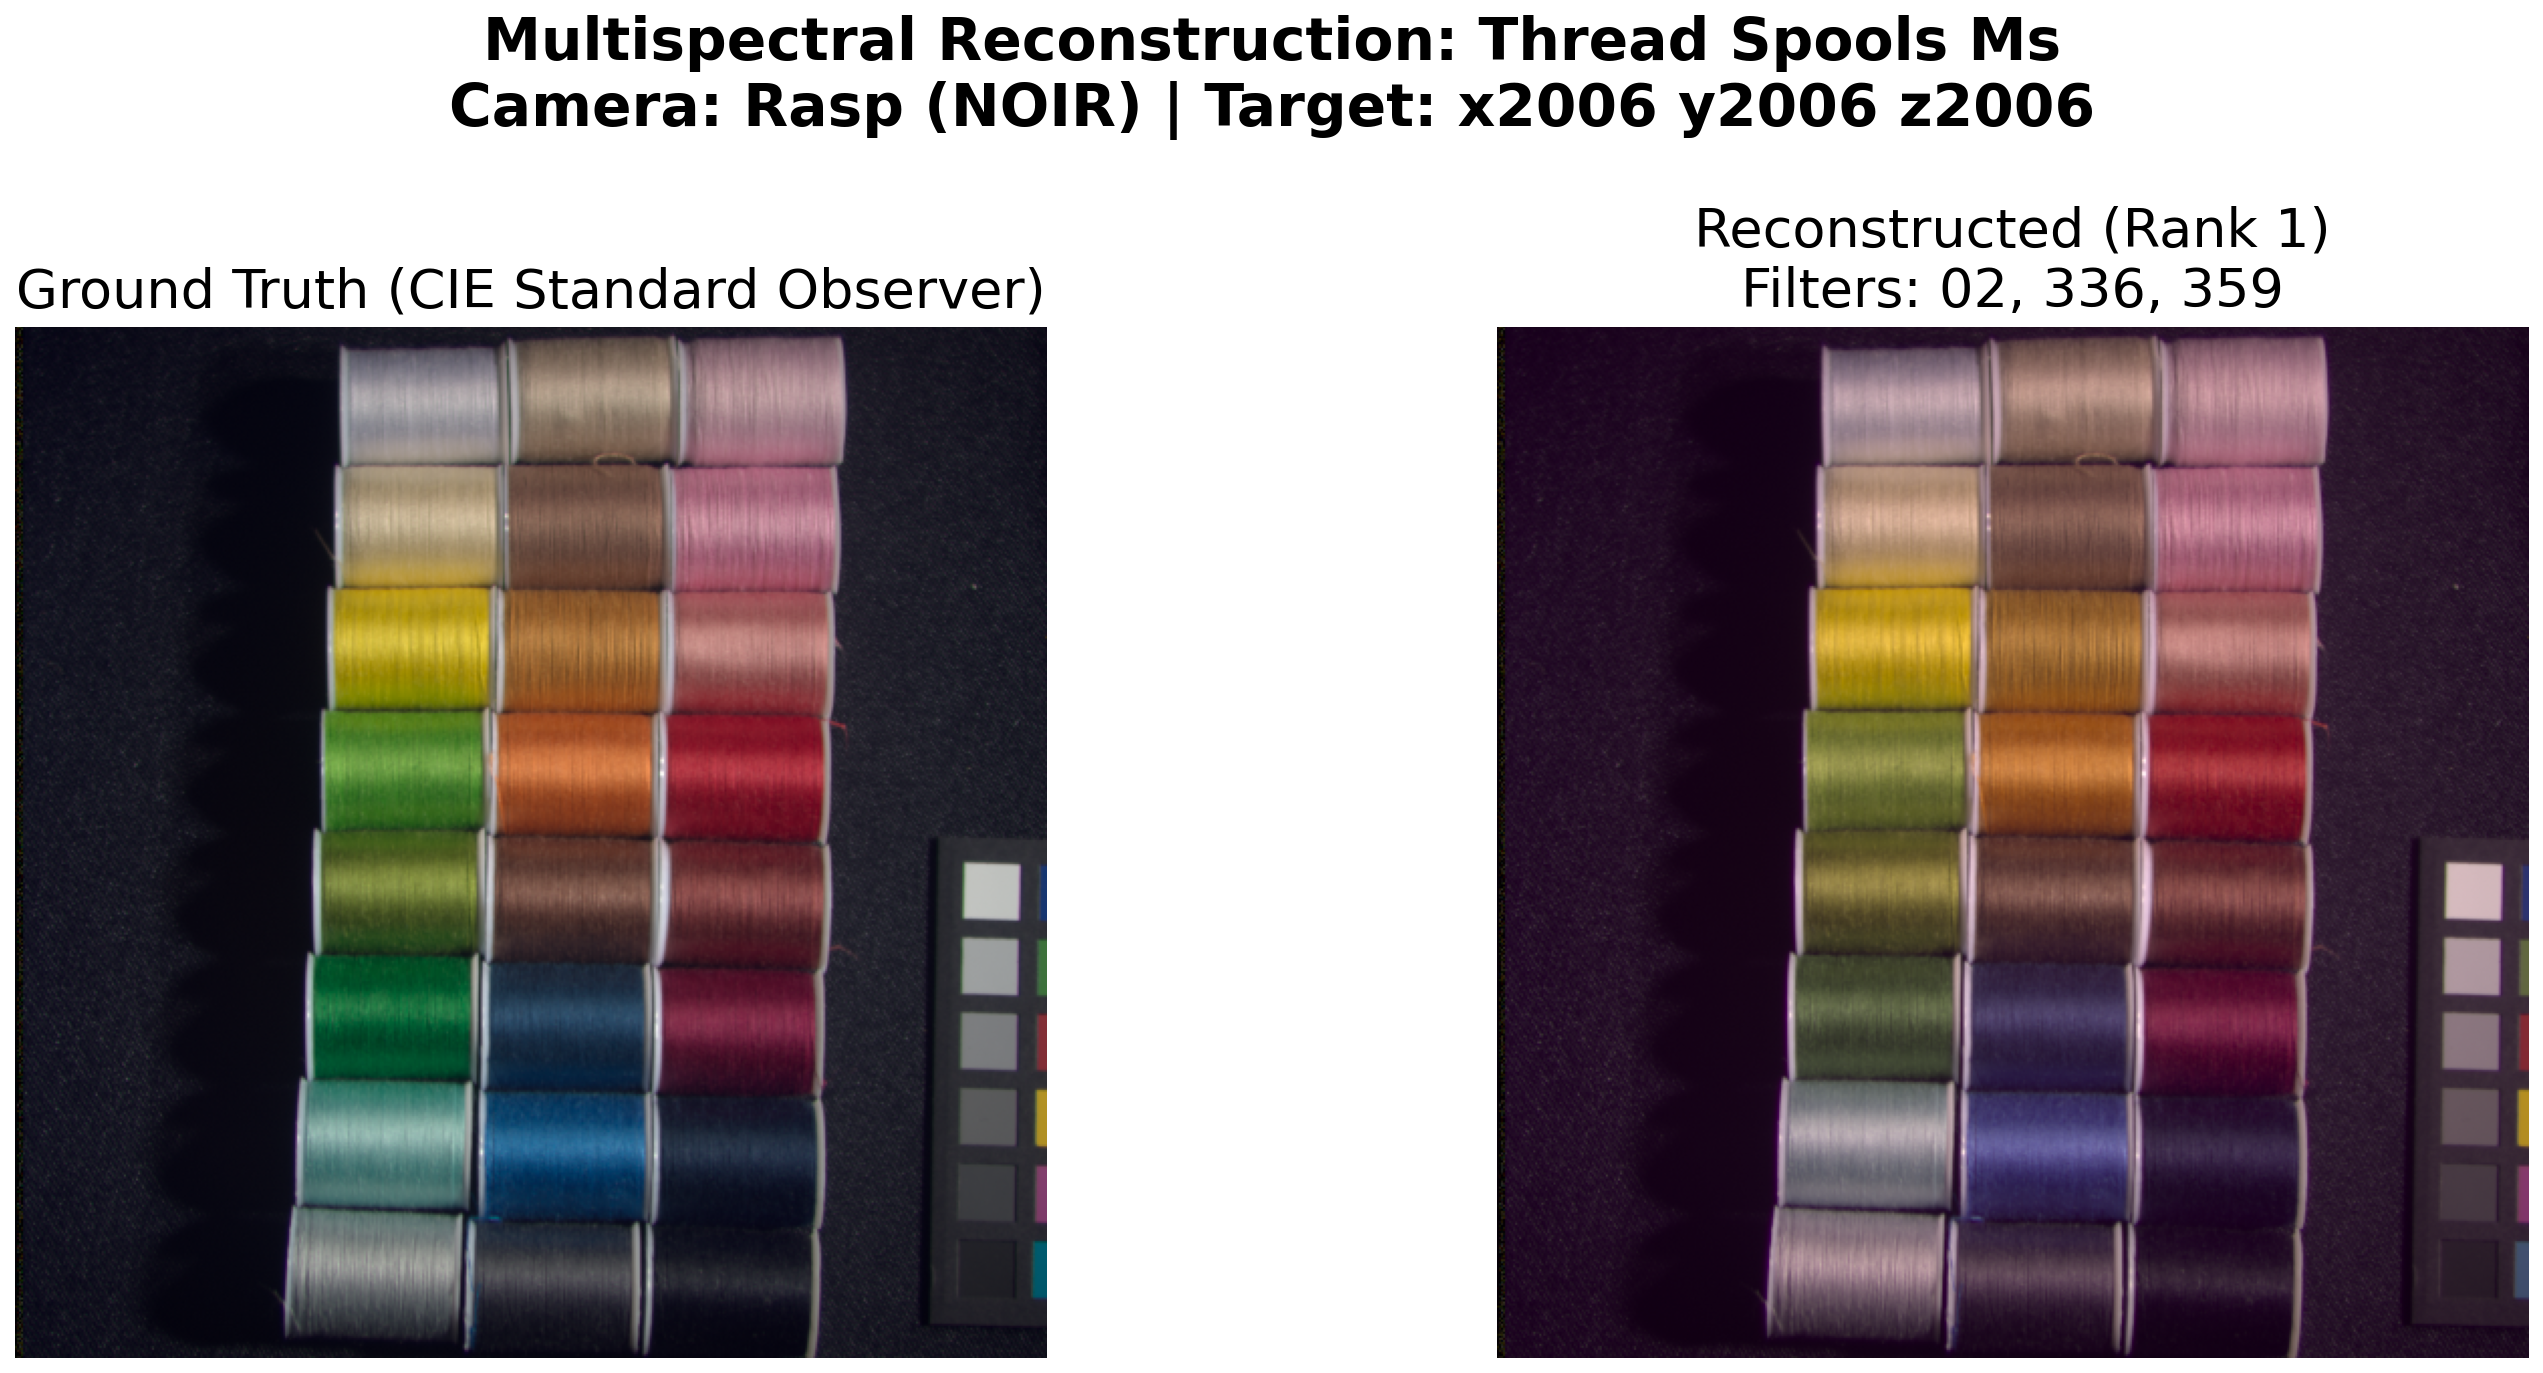
\includegraphics[width=\linewidth]{media/measured_k3_cave.png}
    \caption{CAVE render of combination}
\end{subfigure}
\caption{Supergel results for $k=3$.}
\label{fig:k3spectral}
\end{figure}

We also include some characteristics of the filters themselves, specifically the 1931 gamut locations and their measured transmission functions. 

\begin{figure}[H]
\centering
\begin{subfigure}{.40\linewidth}
    \centering
    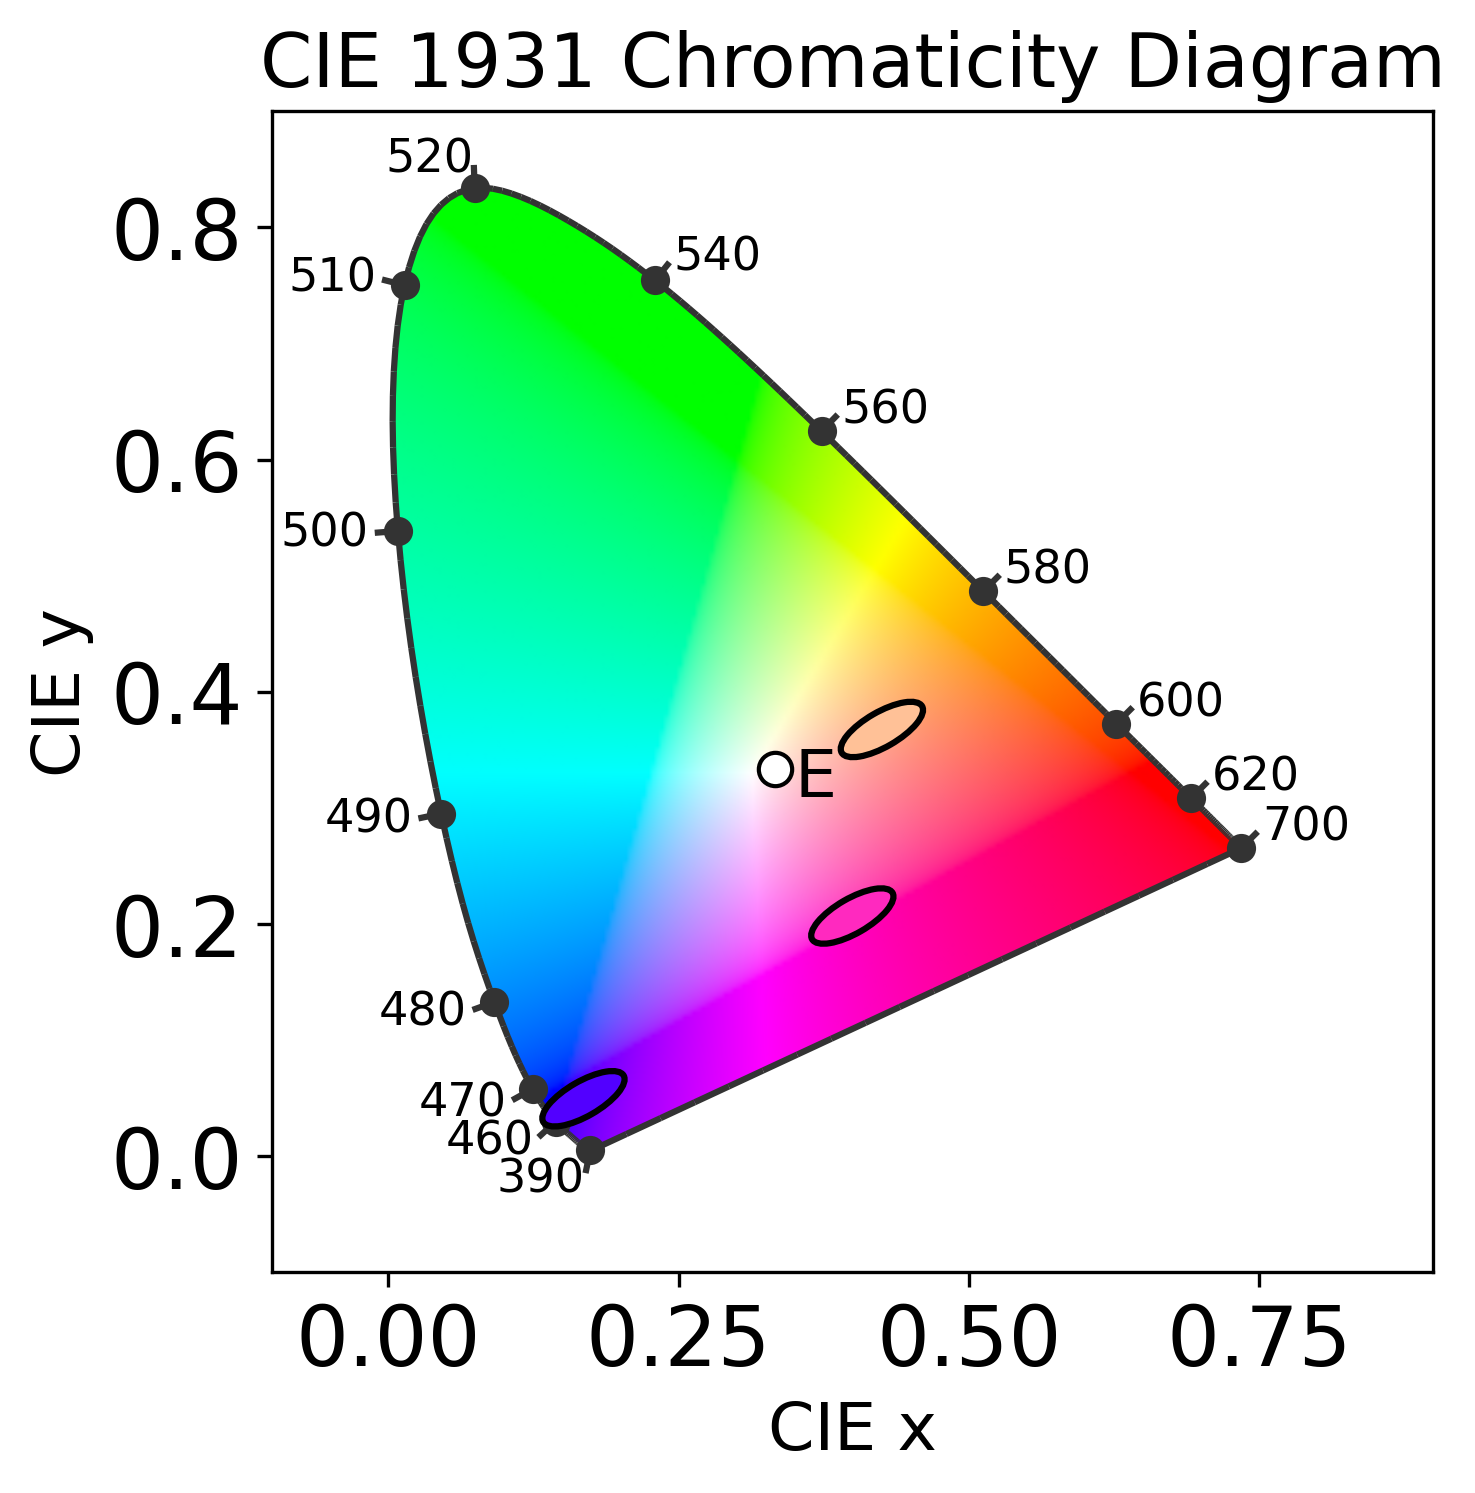
\includegraphics[width=\linewidth]{media/measured_k3_gamut.png}
    \caption{Location on CIE 1931 Color Gamut}
\end{subfigure}%
\begin{subfigure}{.55\linewidth}
    \centering
    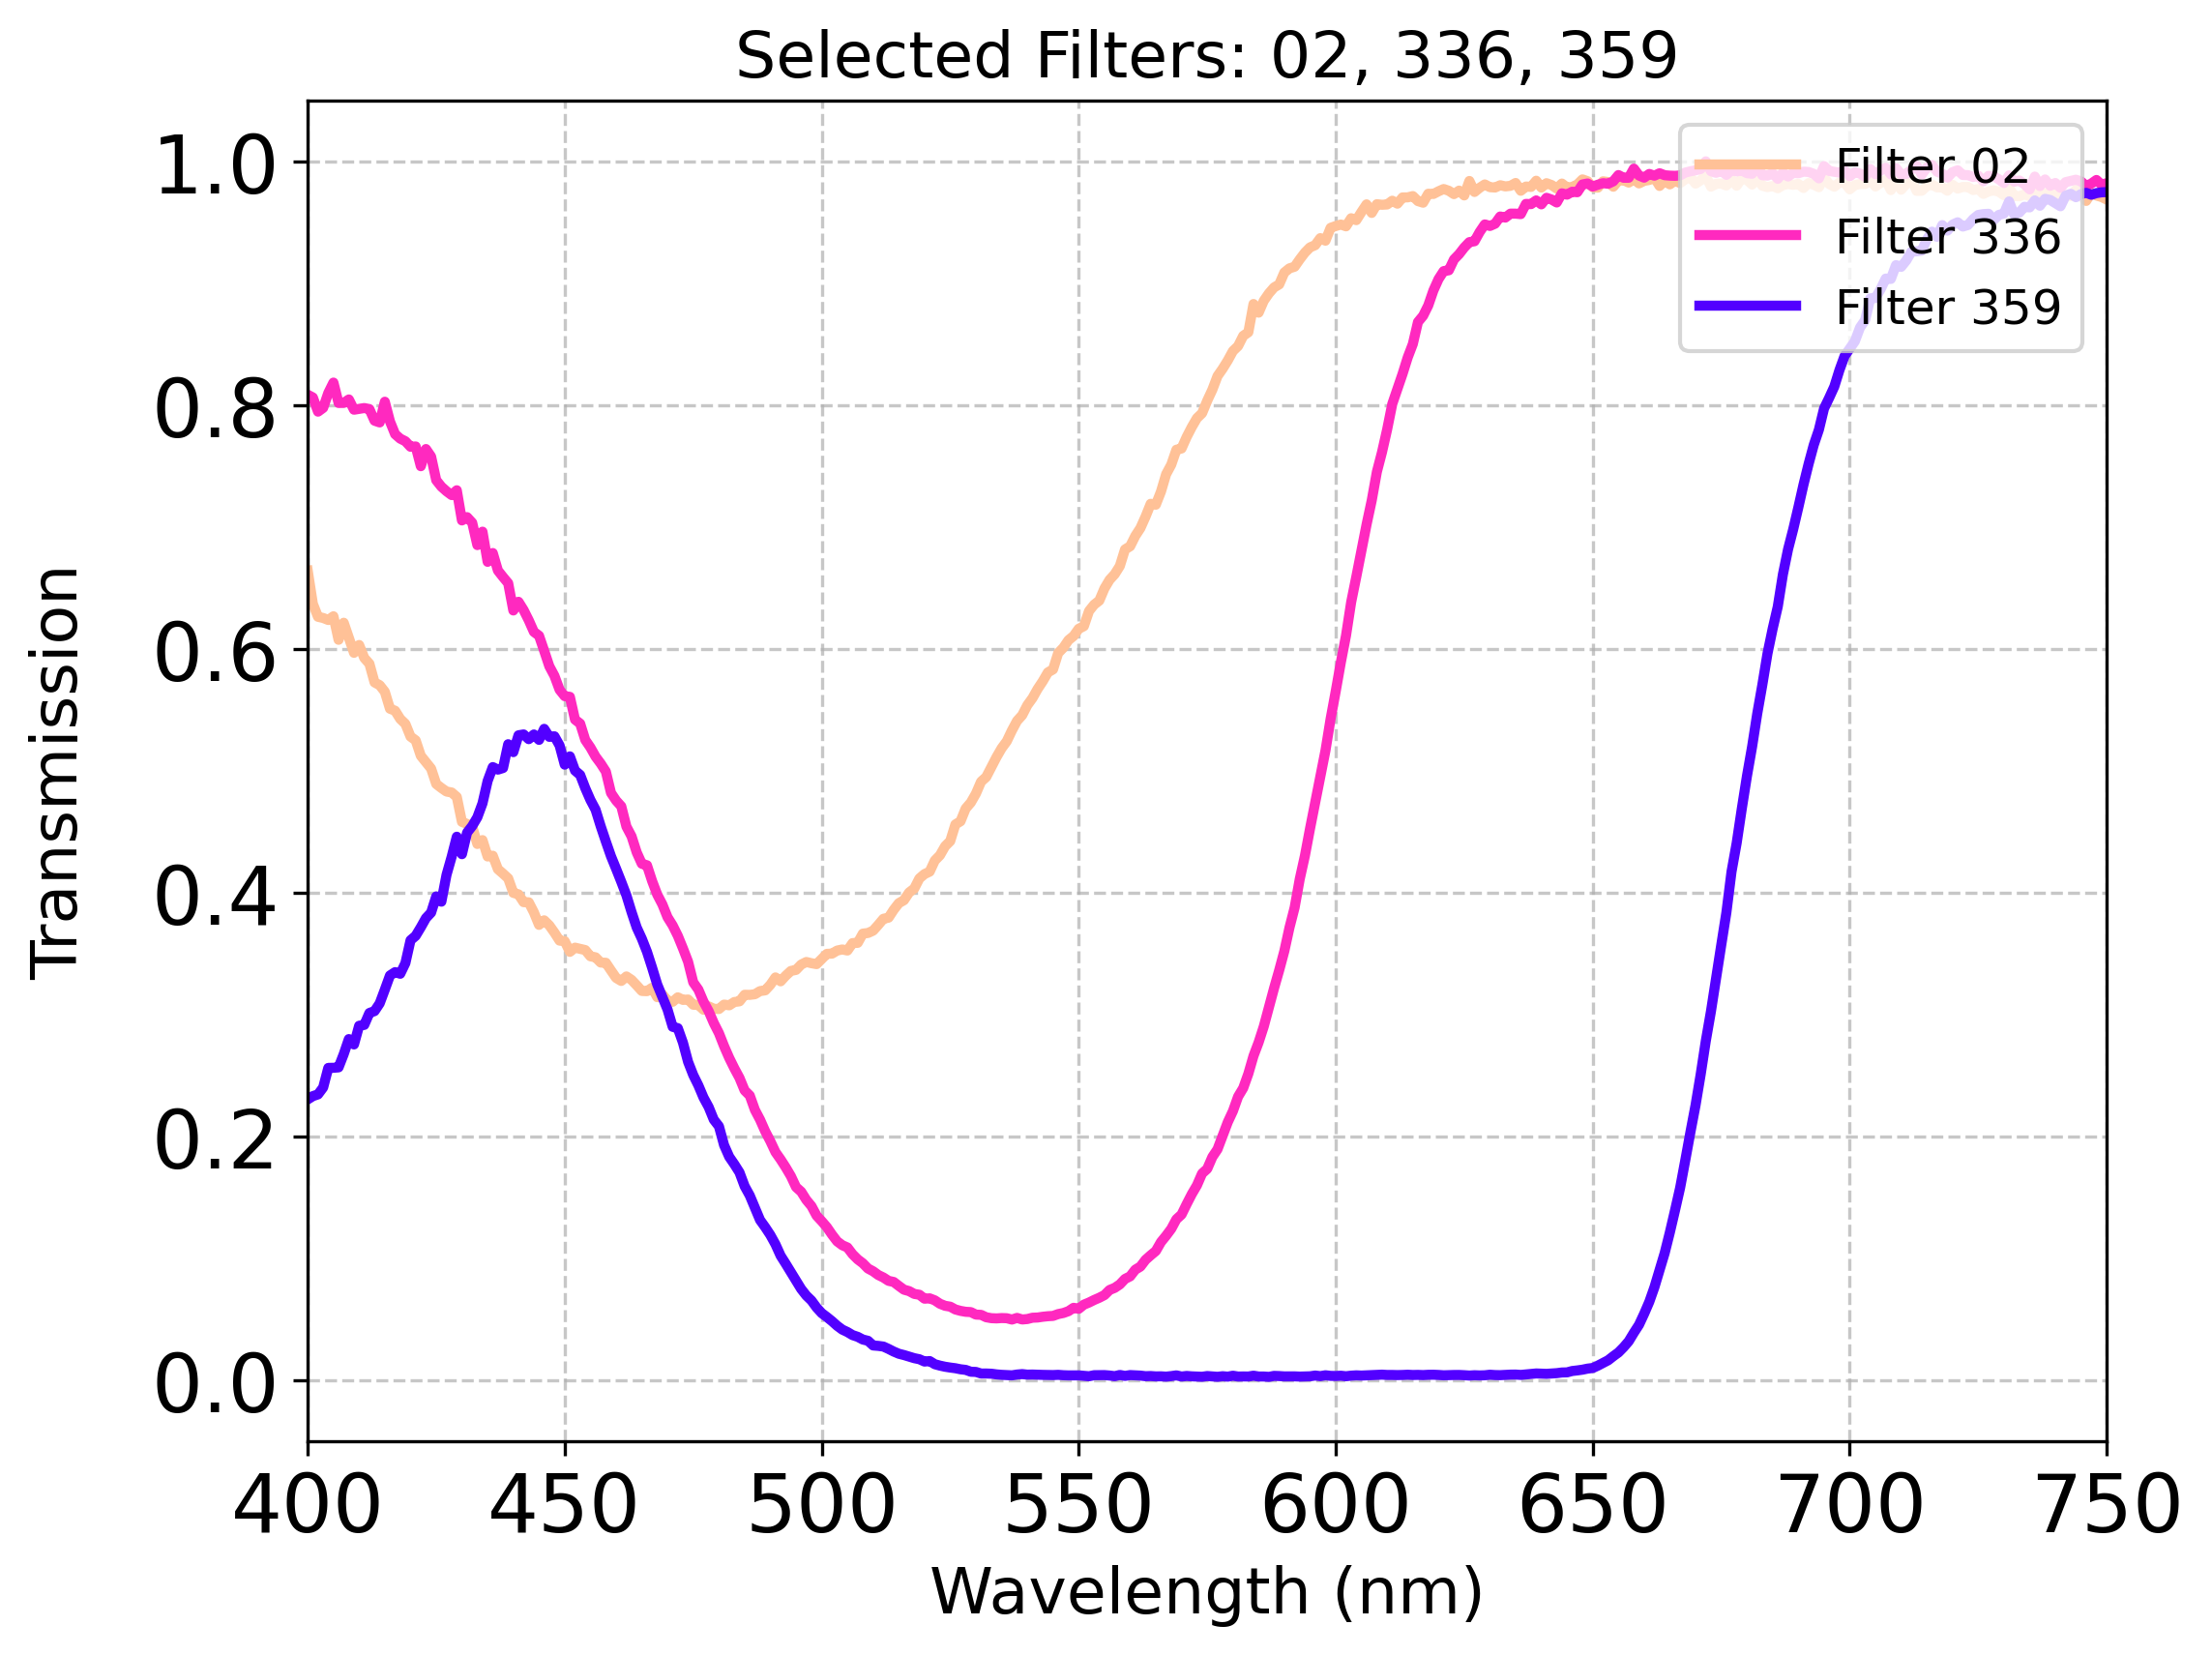
\includegraphics[width=\linewidth]{media/measured_k3_trans.png}
    \caption{Transmission functions of selected filters}
\end{subfigure}
\caption{$k=3$ Transmission functions and location on gamut}
\label{fig:k3Transmissions}
\end{figure}

\subsubsection{Solution for $k=4$}

We see a noticeable improvement in MSE and in $\dE$ with $k=4$, measuring 1.09, slightly above the 'just noticeable difference' of 1.0 \cite{lindstrom2008delta}. 
The CAVE dataset reconstruction approaches the ground truth reconstruction, although the human eye may observe slight differences in the overall image. 

\begin{figure}[H]
\centering
\begin{subfigure}{.49\linewidth}
    \centering
    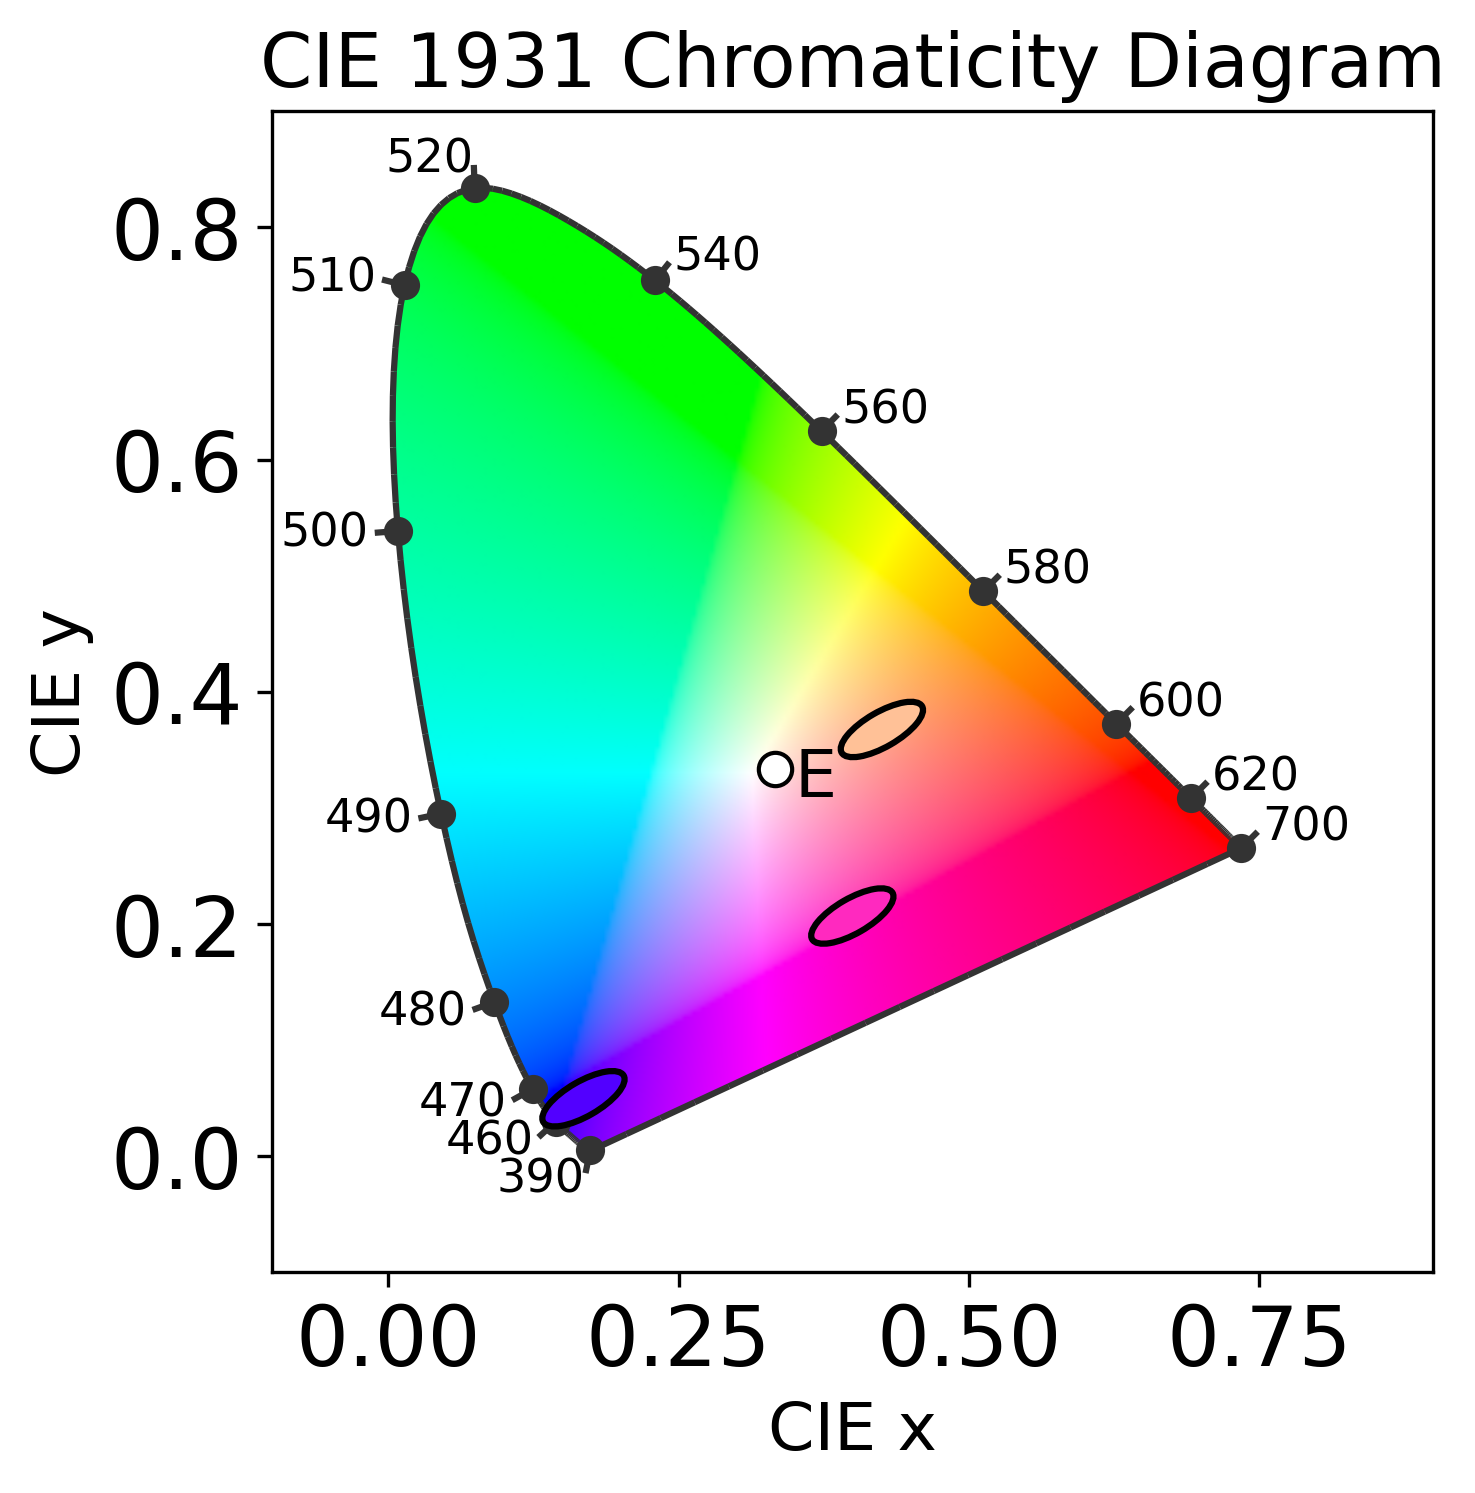
\includegraphics[width=\linewidth]{media/measured_k3_gamut.png}
    \caption{Best XYZ reconstruction}
\end{subfigure}%
\begin{subfigure}{.49\linewidth}
    \centering
    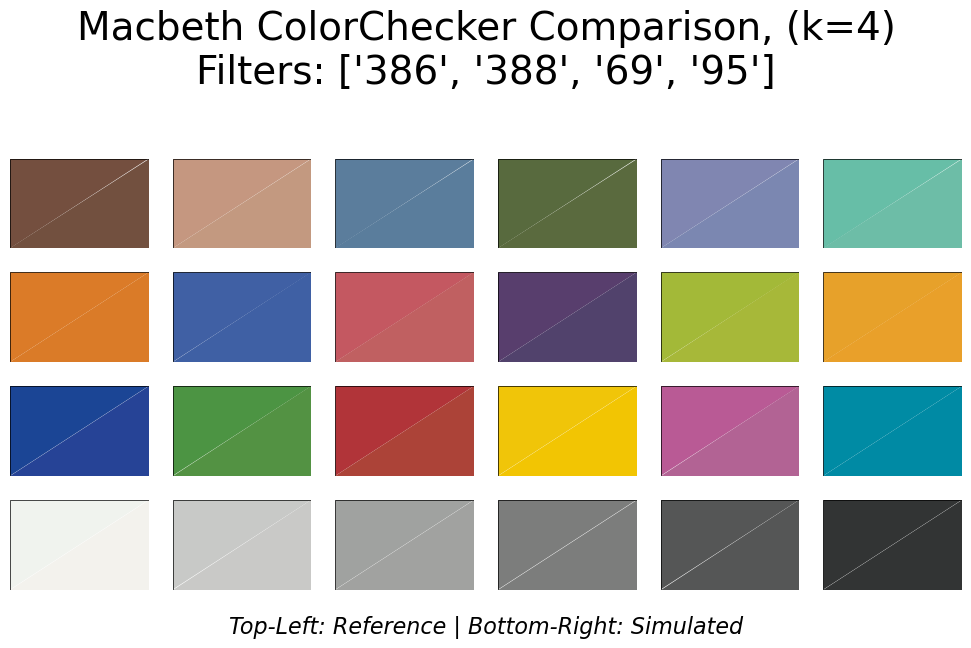
\includegraphics[width=\linewidth]{media/measured_k4_macbeth.png}
    \caption{Macbeth Color Checker comparison}
\end{subfigure}
\begin{subfigure}{.49\linewidth}
    \centering
    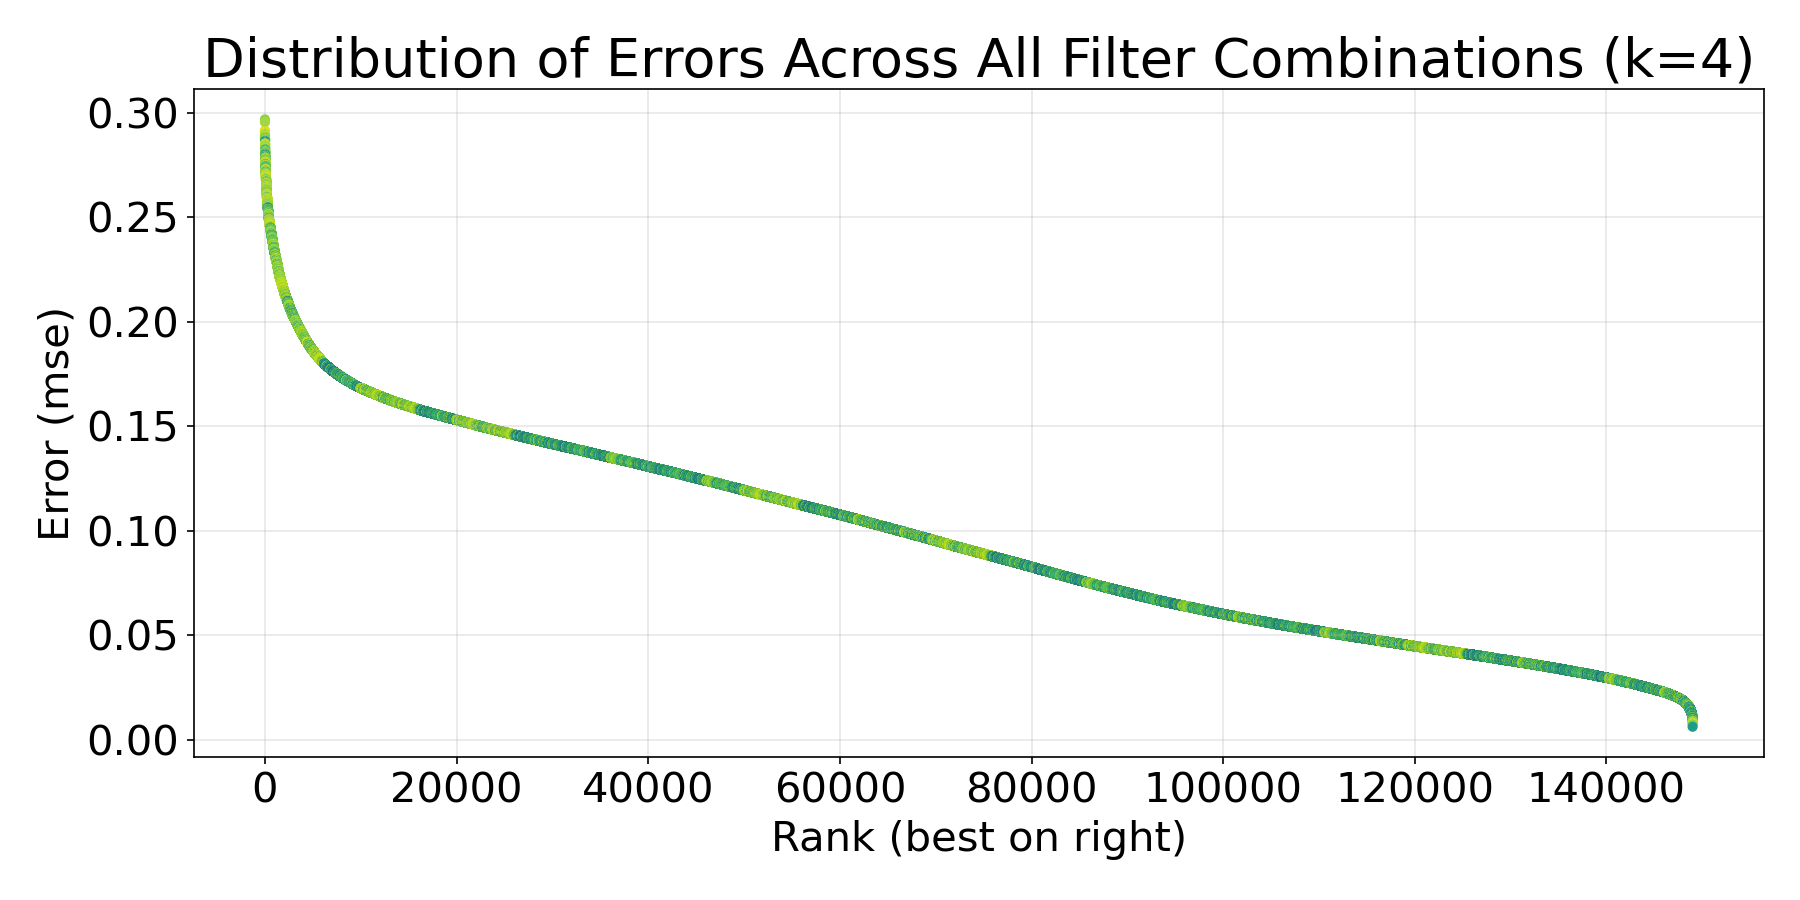
\includegraphics[width=\linewidth]{media/measured_k4_errors.png}
    \caption{Error distribution across combinations}
\end{subfigure}%
\begin{subfigure}{.49\linewidth}
    \centering
    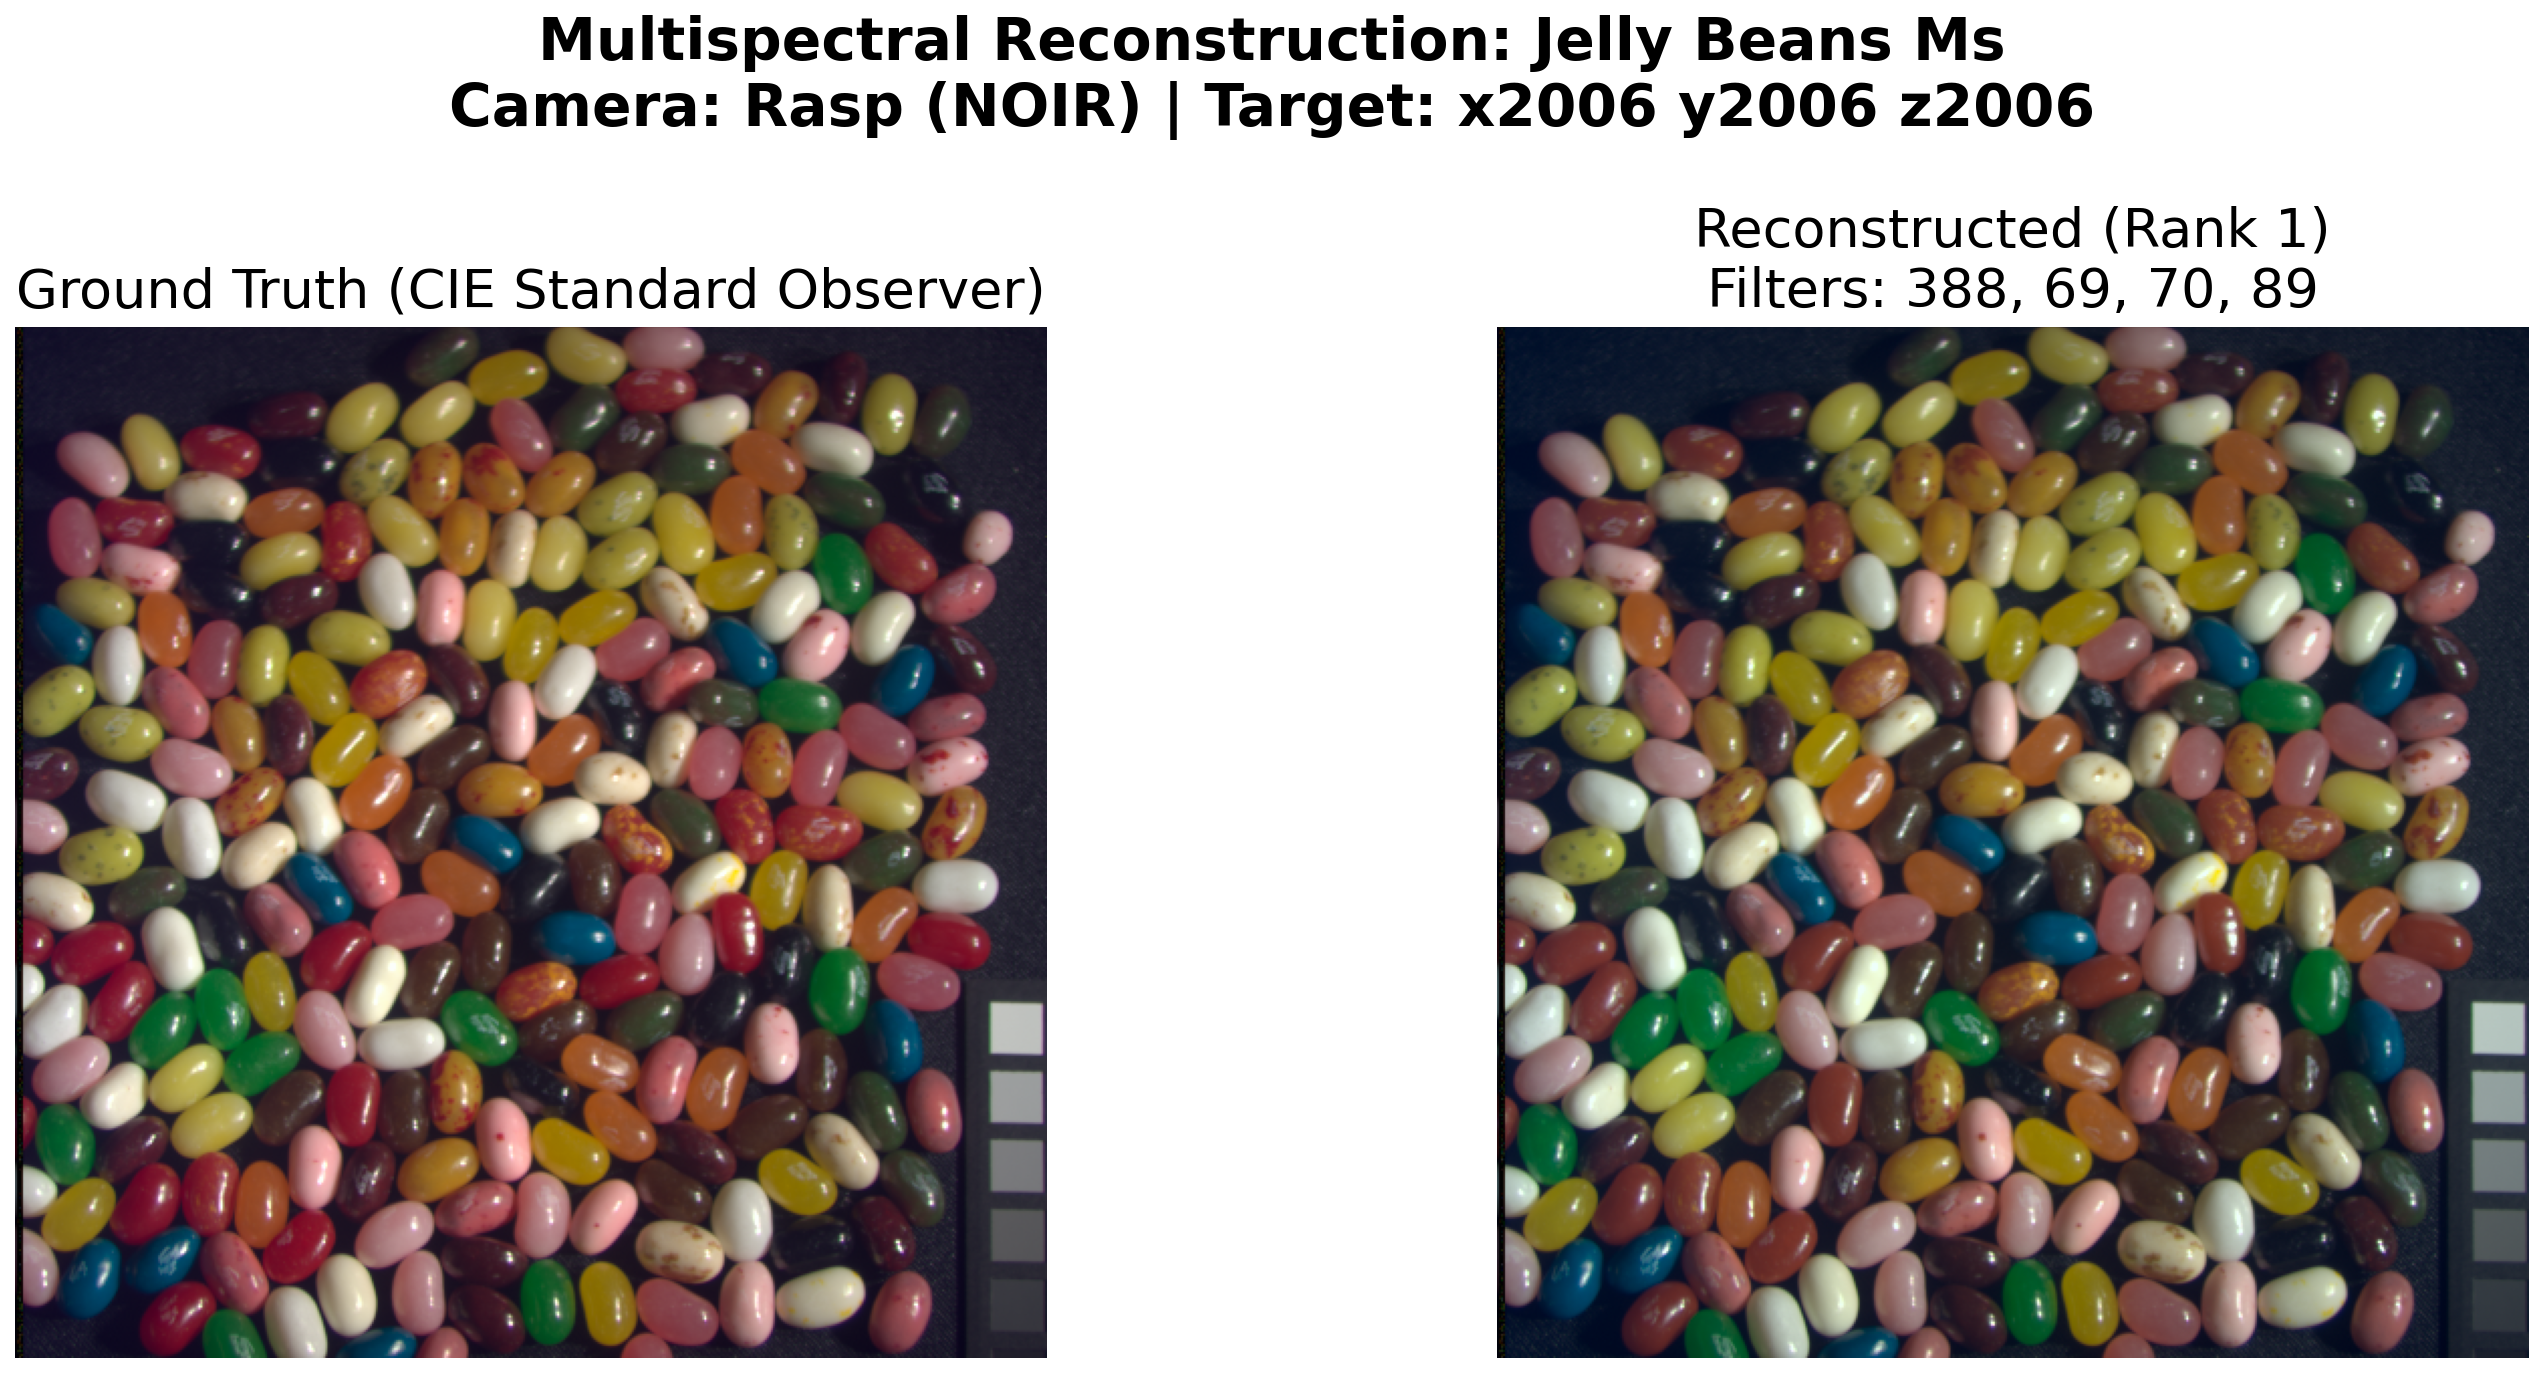
\includegraphics[width=\linewidth]{media/measured_k4_cave.png}
    \caption{CAVE render of combination}
\end{subfigure}
\caption{Supergel results for $k=4$.}
\label{fig:k4spectral}
\end{figure}

In comparison to the $k=3$ case, we see relatively little transmission above the 650nm range, yet a reconstruction may struggle to recreate red hues and the 15th Macbeth patch, the dark red patch, has a $\dE$ of about 9, significantly worse than the rest. 
Conceptually, we can see that the gamut has little coverage over the red corner of the 1931 color gamut.

\begin{figure}[H]
\centering
\begin{subfigure}{.40\linewidth}
    \centering
    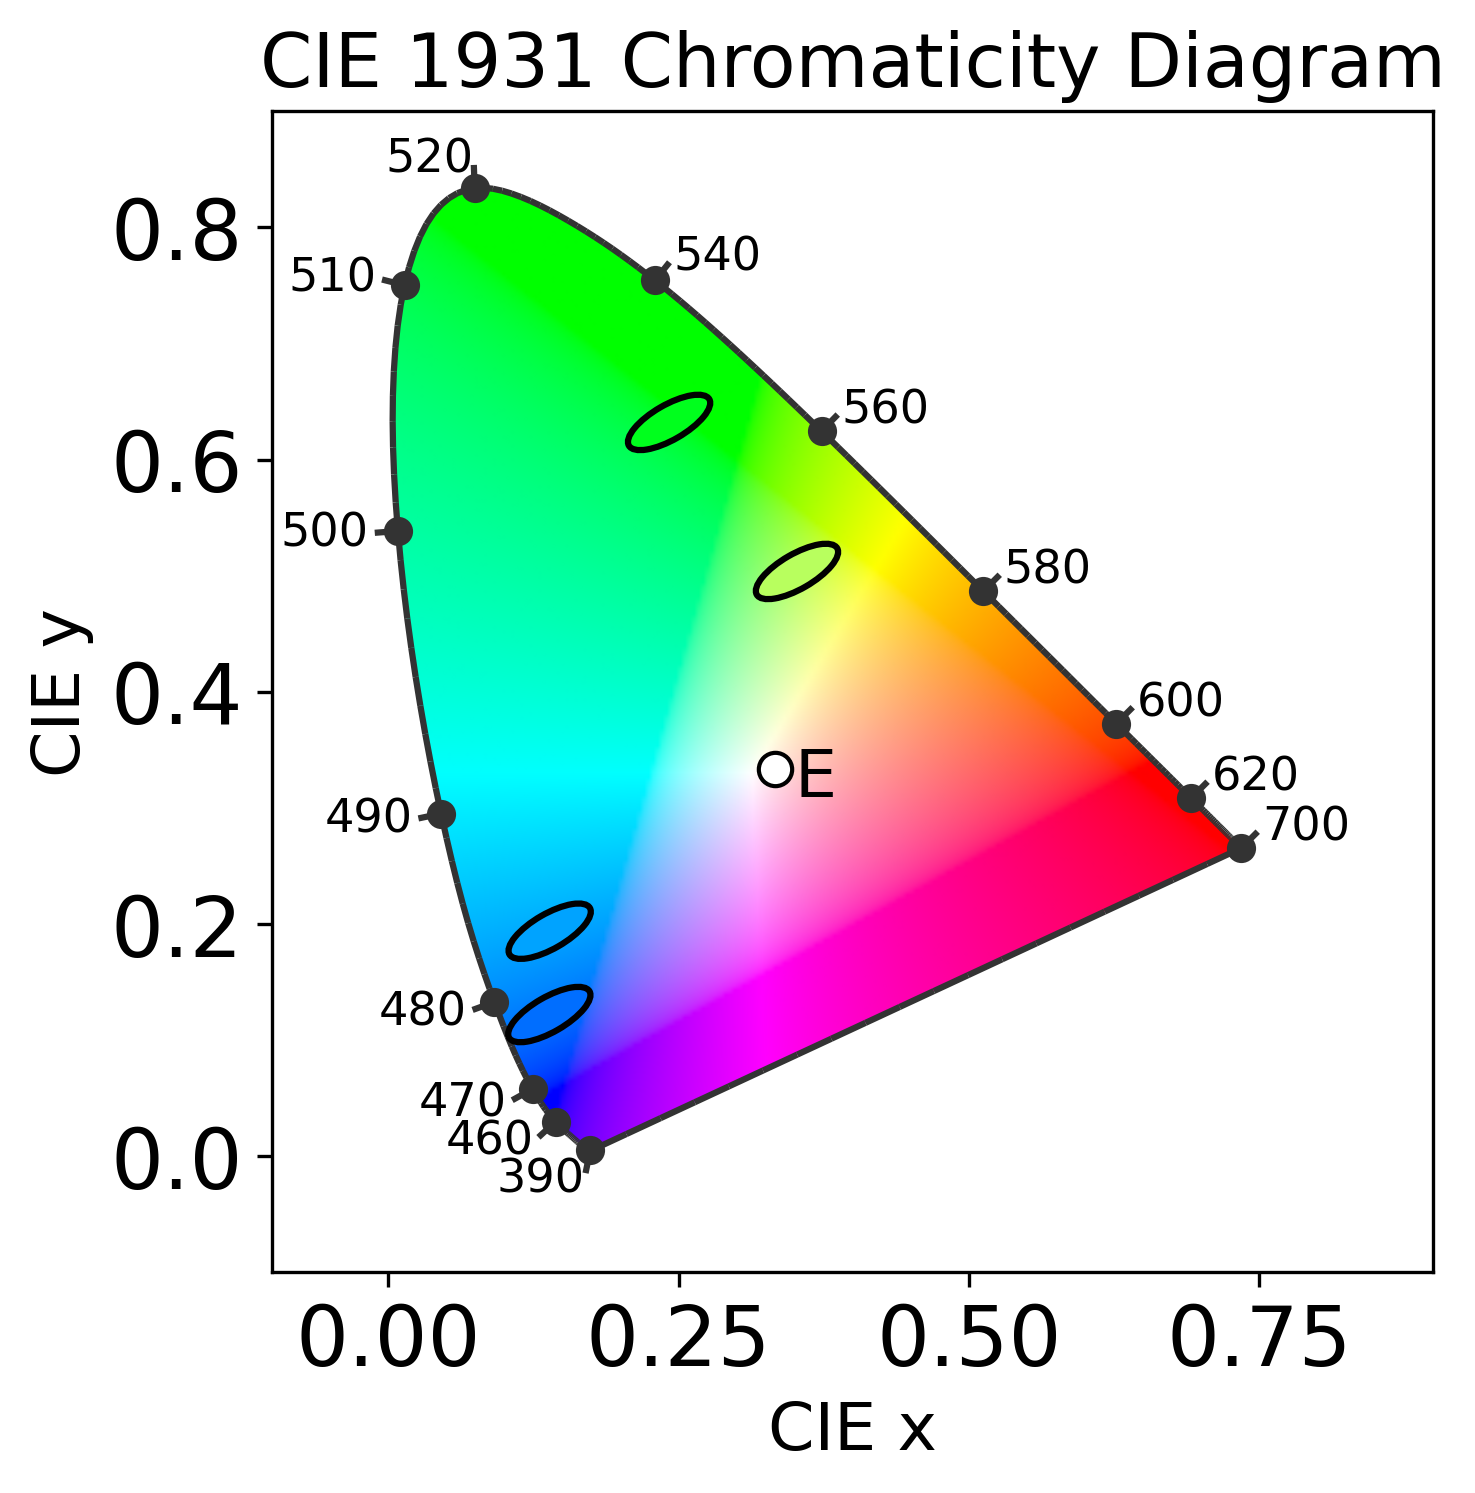
\includegraphics[width=\linewidth]{media/measured_k4_gamut.png}
    \caption{Location on CIE 1931 Color Gamut}
\end{subfigure}%
\begin{subfigure}{.55\linewidth}
    \centering
    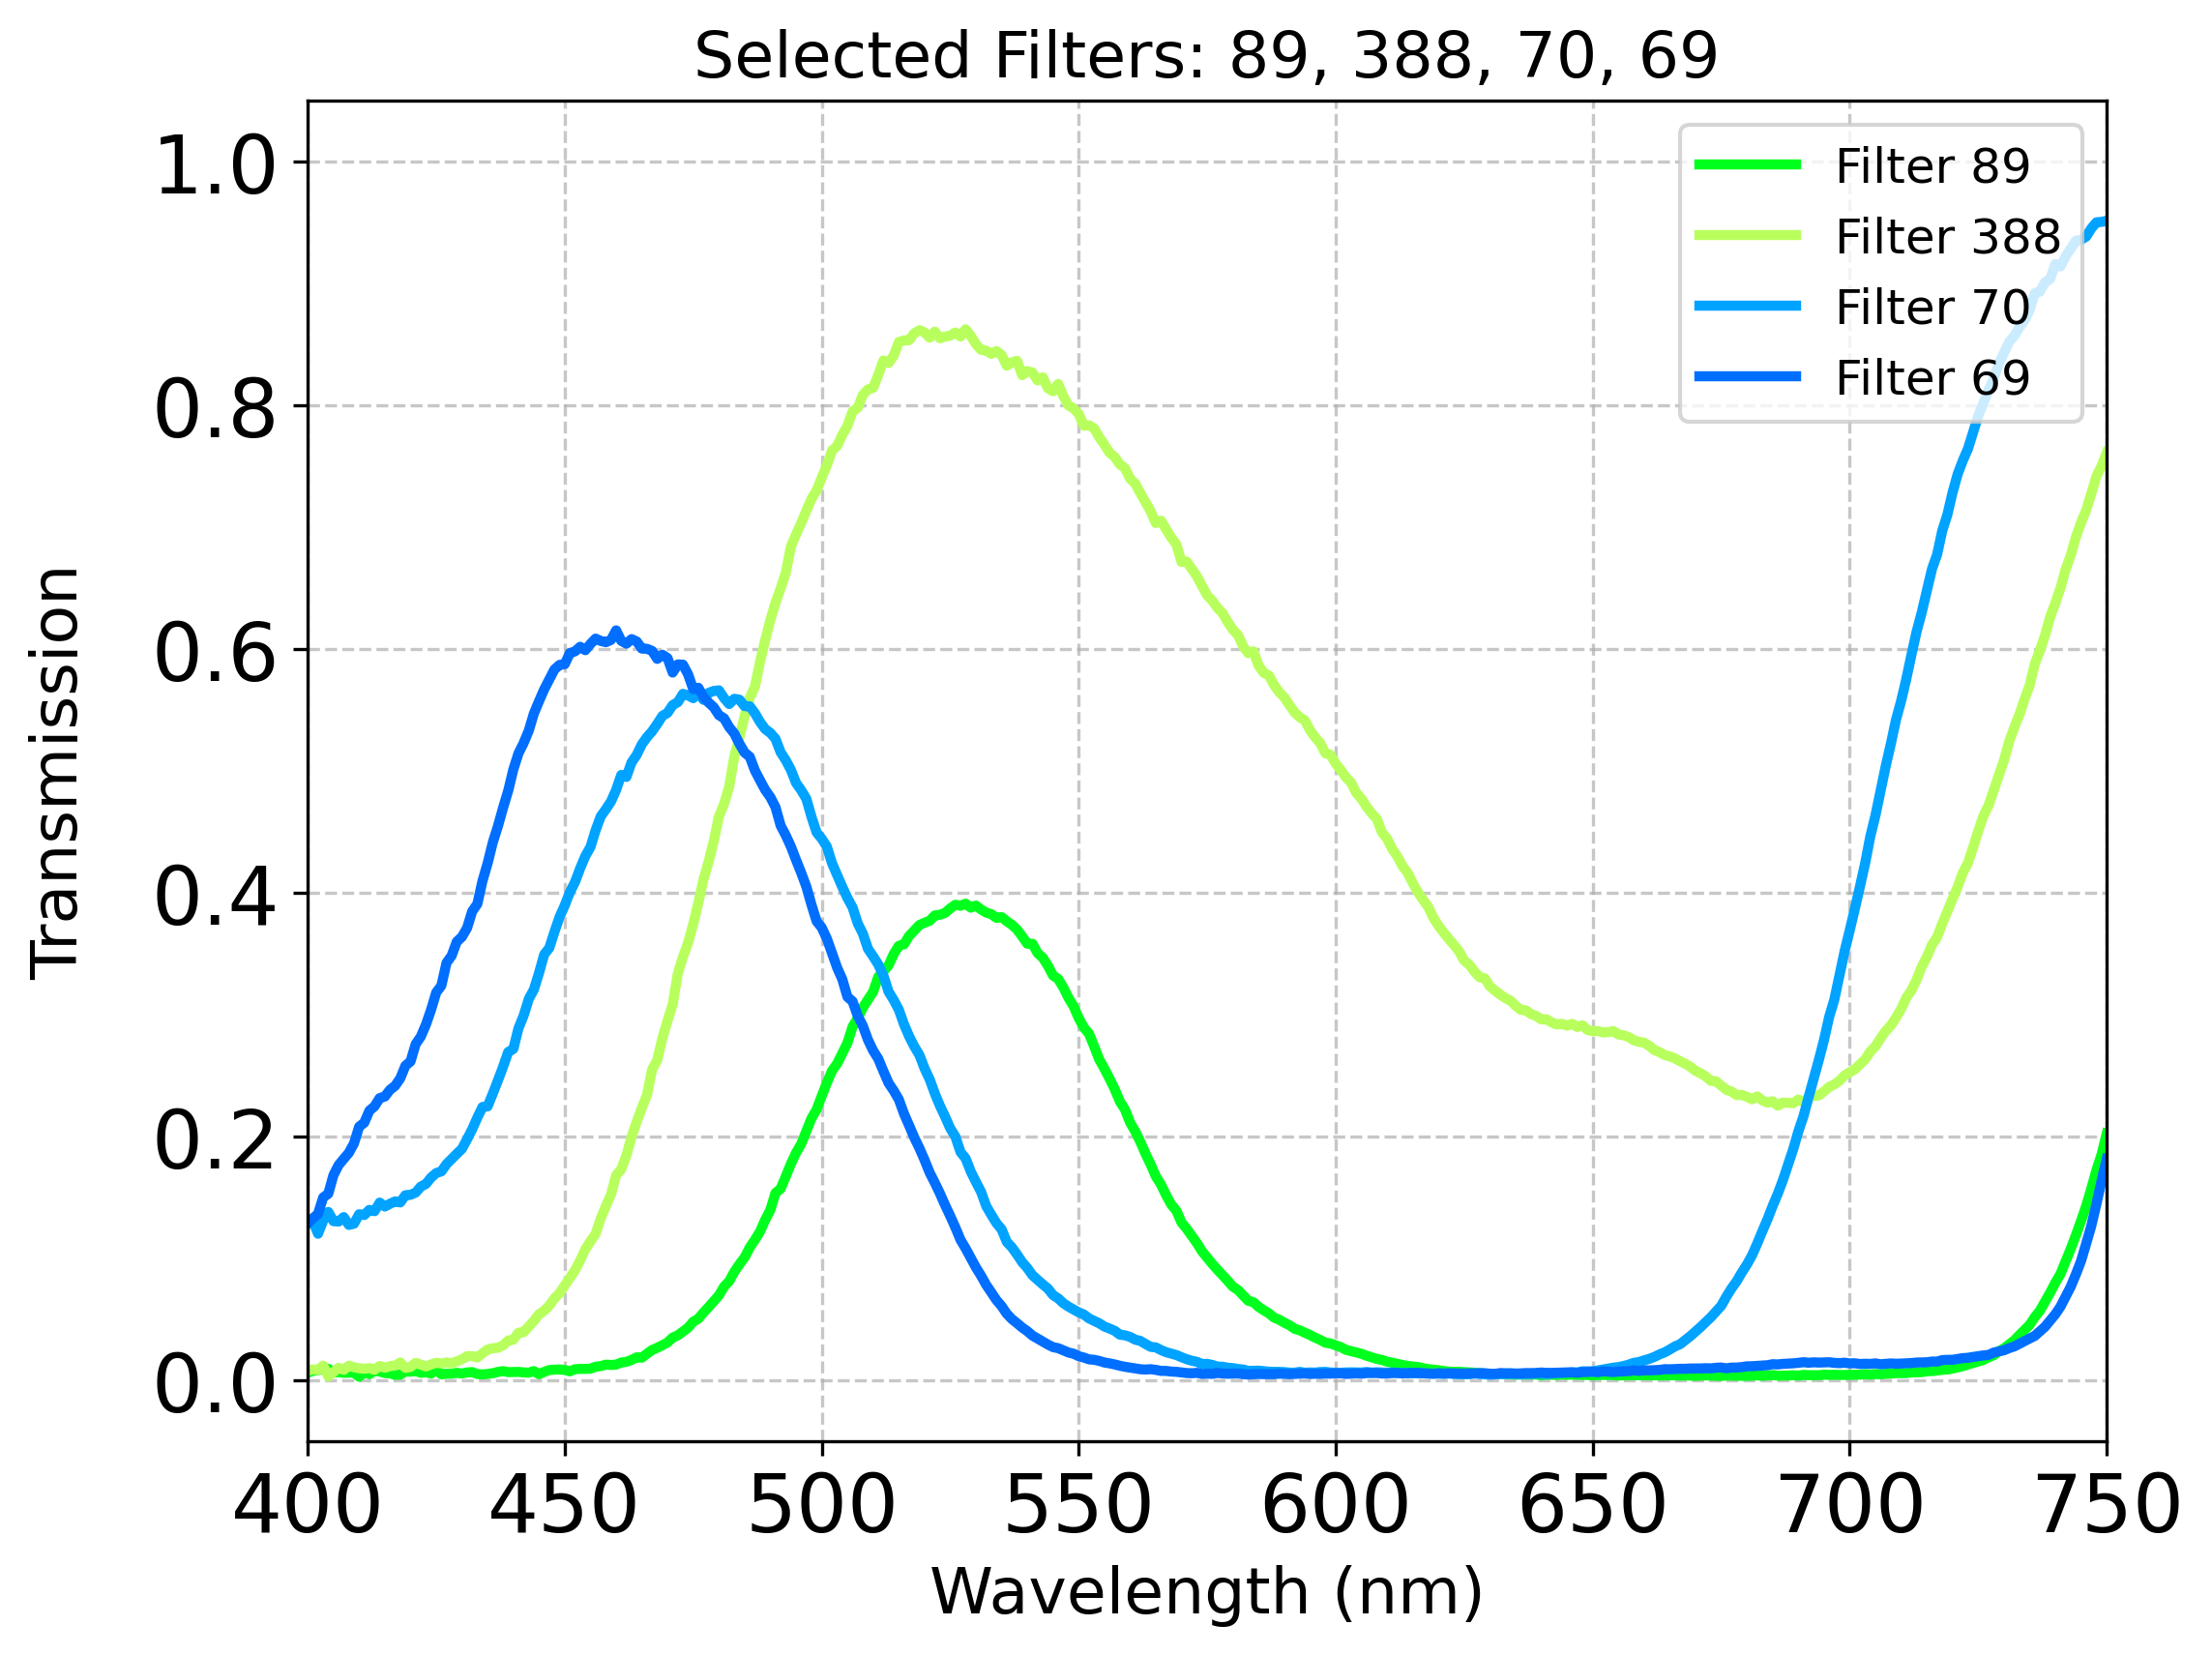
\includegraphics[width=\linewidth]{media/measured_k4_transmission.png}
    \caption{Transmission functions of selected filters}
\end{subfigure}
\caption{$k=4$ Transmission functions and location on gamut}
\label{fig:k4Transmissions}
\end{figure}

\subsubsection{Solution for $k=5$}


For the $k=5$ case, the $\dE$ reaches .35 and clearly improves on the reconstruction of the target curves. 
Importantly, the worst individual $\dE$ recorded amongst the Macbeth patches are patches 2 and 15, the tan and red patches. 
The cave reconstruction is quite hard to distinguish from the ground truth. 

\begin{figure}[H]
\centering
\begin{subfigure}{.49\linewidth}
    \centering
    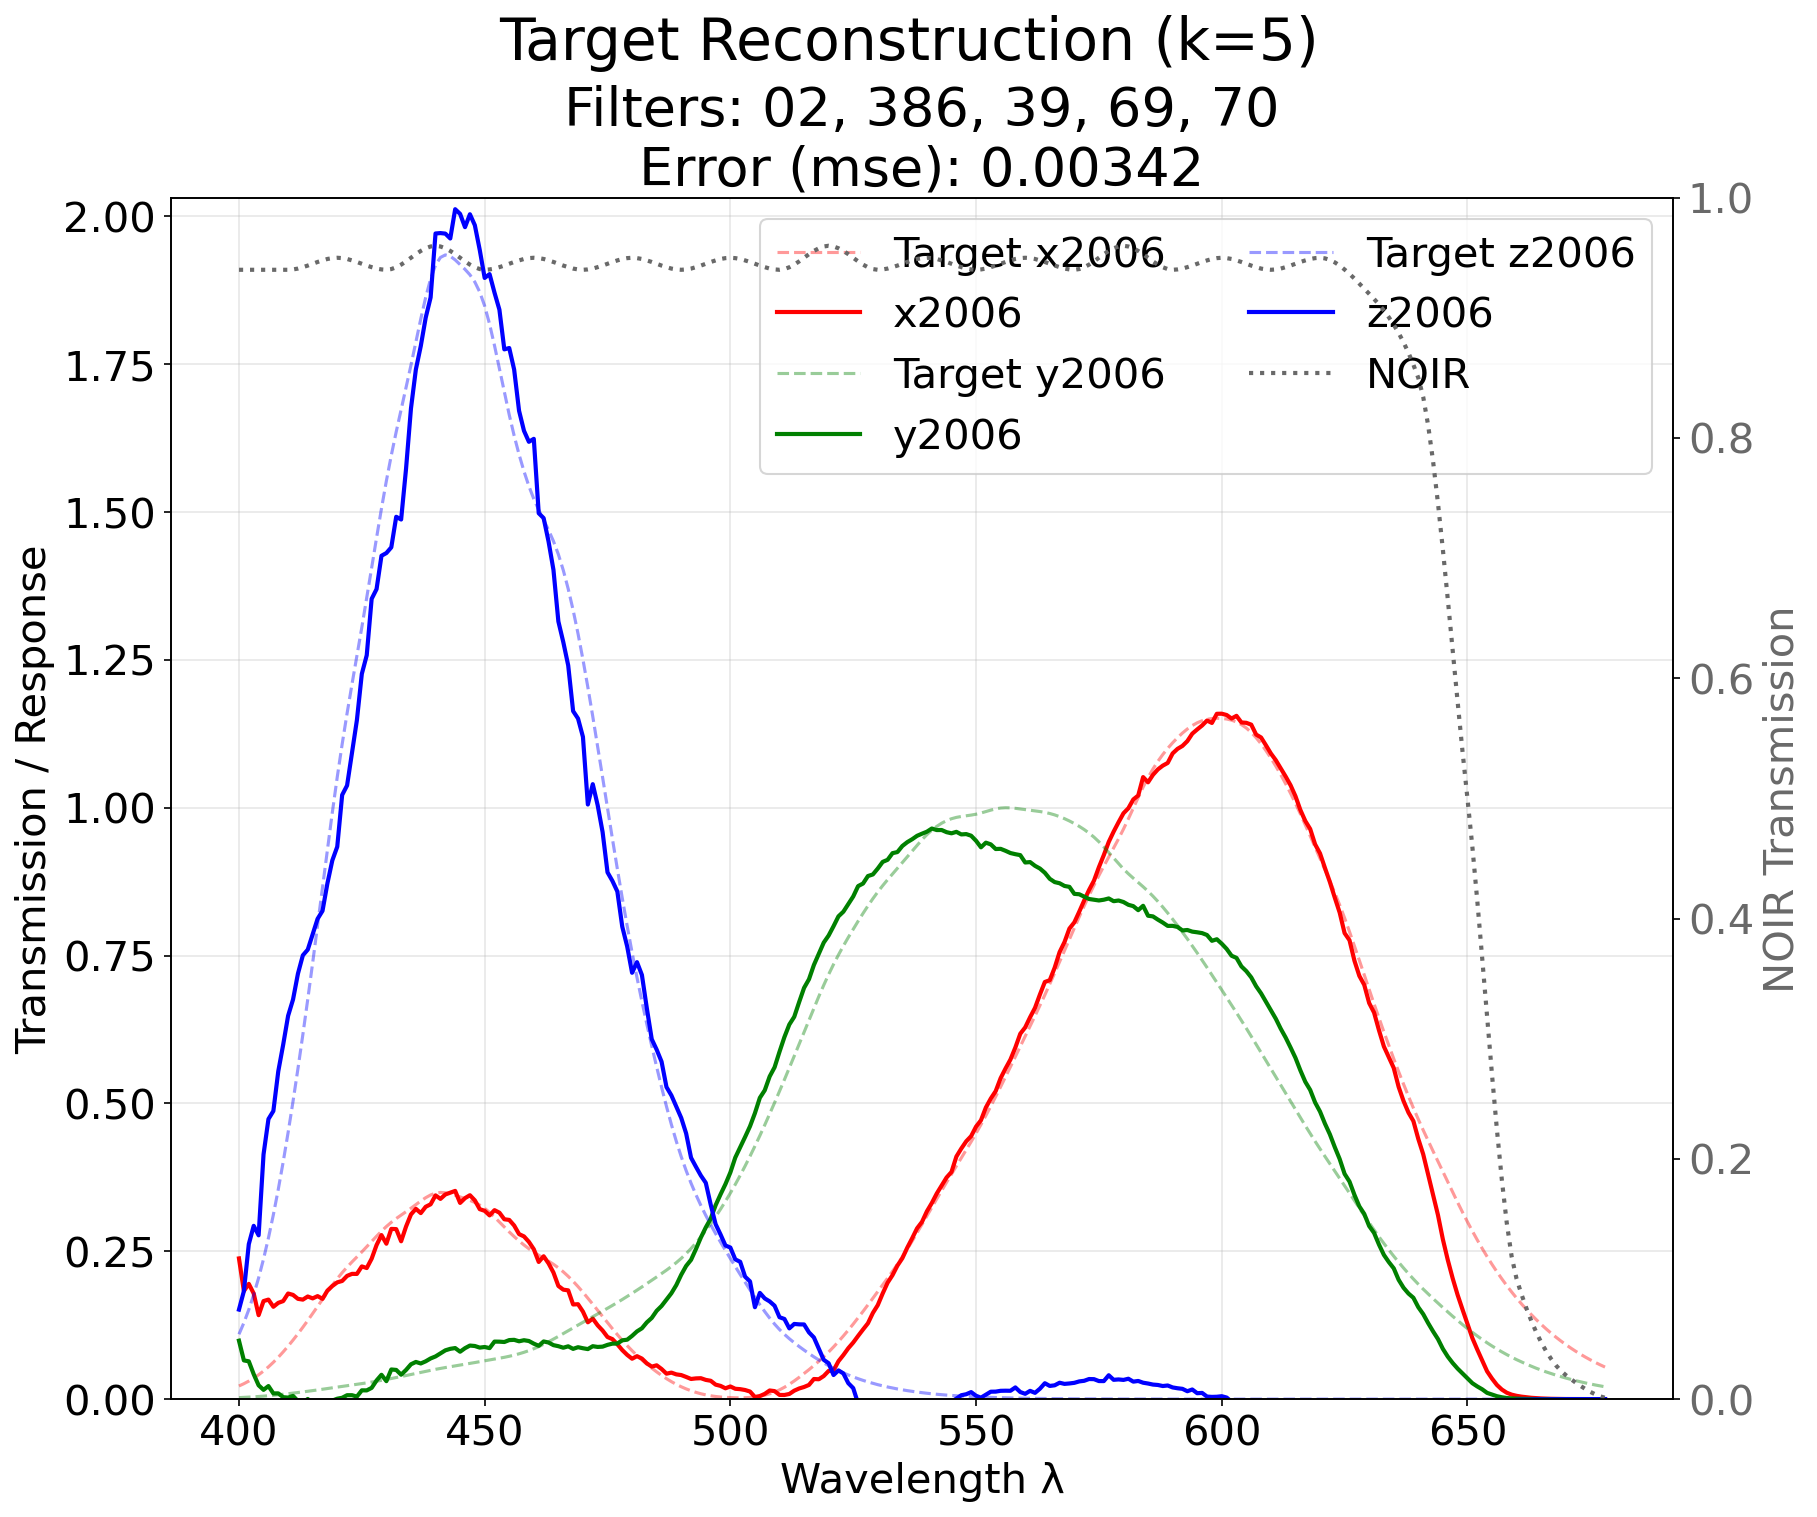
\includegraphics[width=\linewidth]{media/measured_k5_spectra.png}
    \caption{Best XYZ reconstruction}
\end{subfigure}%
\begin{subfigure}{.49\linewidth}
    \centering
    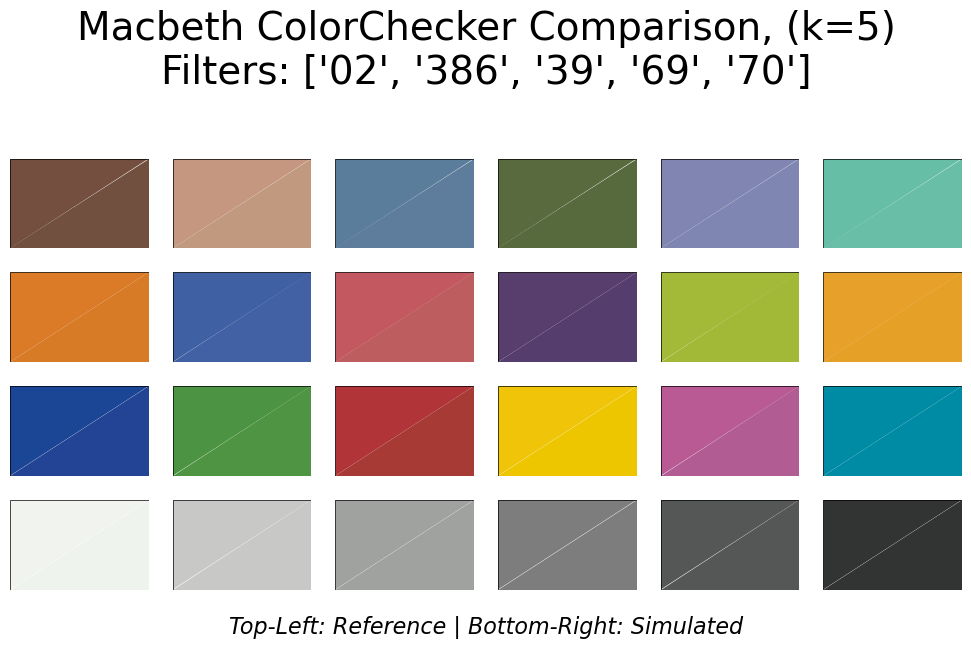
\includegraphics[width=\linewidth]{media/measured_k5_macbeth.png}
    \caption{Macbeth Color Checker comparison}
\end{subfigure}
\begin{subfigure}{.49\linewidth}
    \centering
    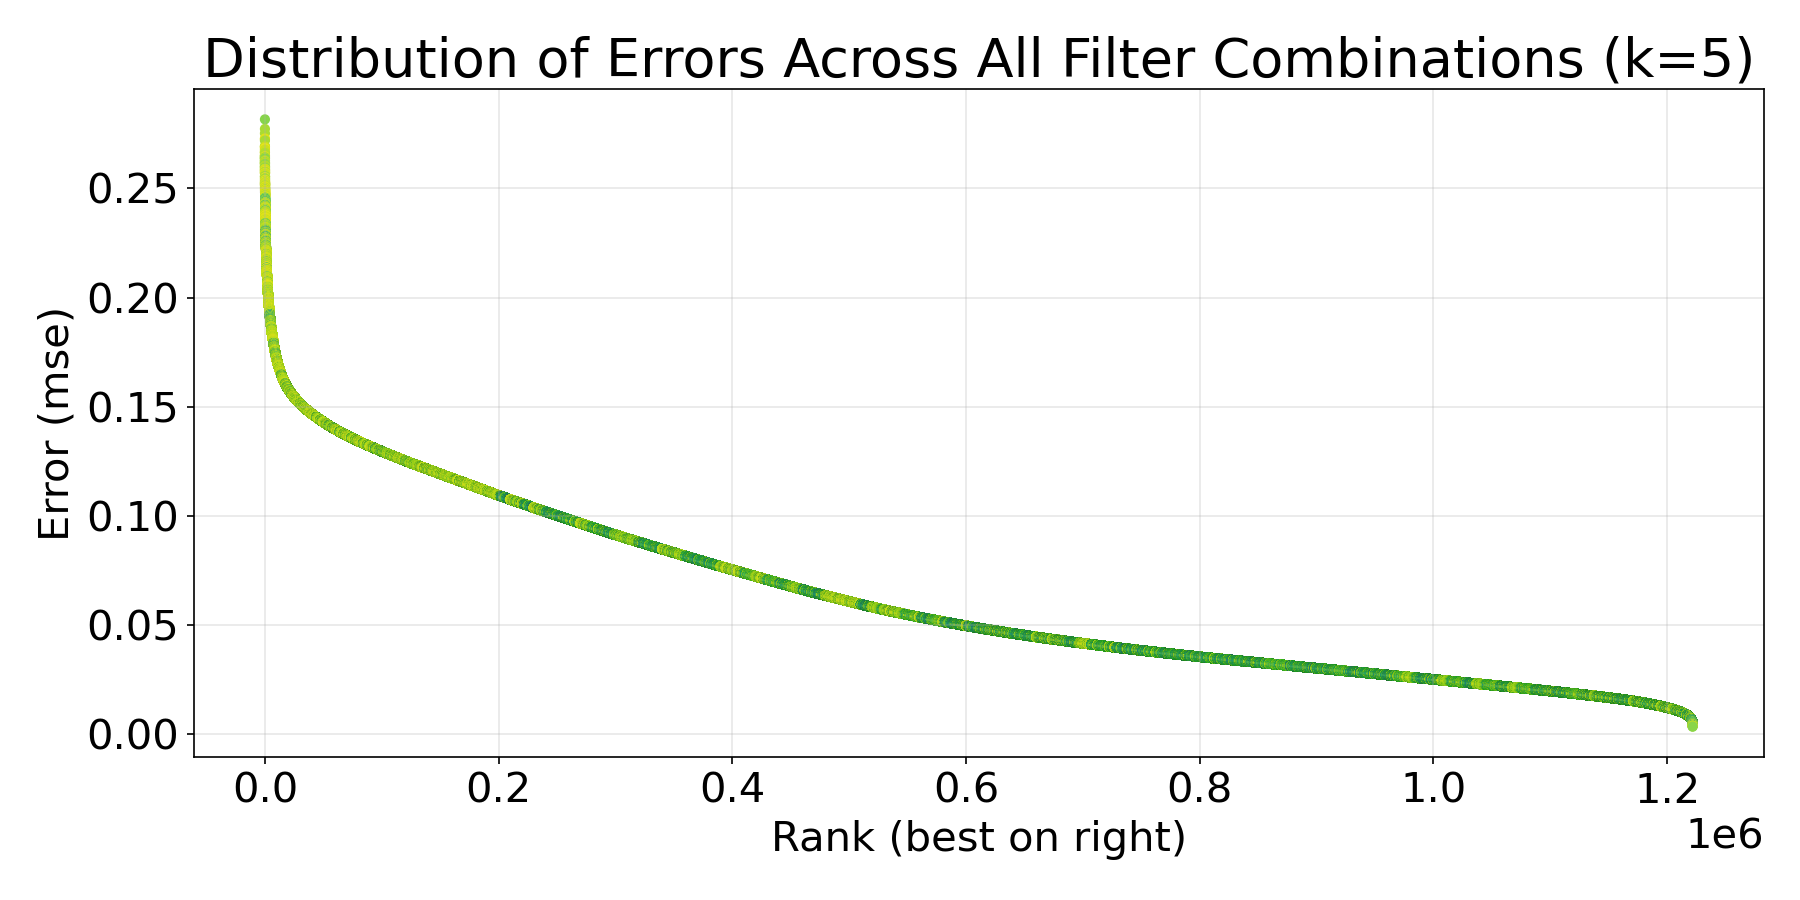
\includegraphics[width=\linewidth]{media/measured_k5_errors.png}
    \caption{Error distribution across combinations}
\end{subfigure}%
\begin{subfigure}{.49\linewidth}
    \centering
    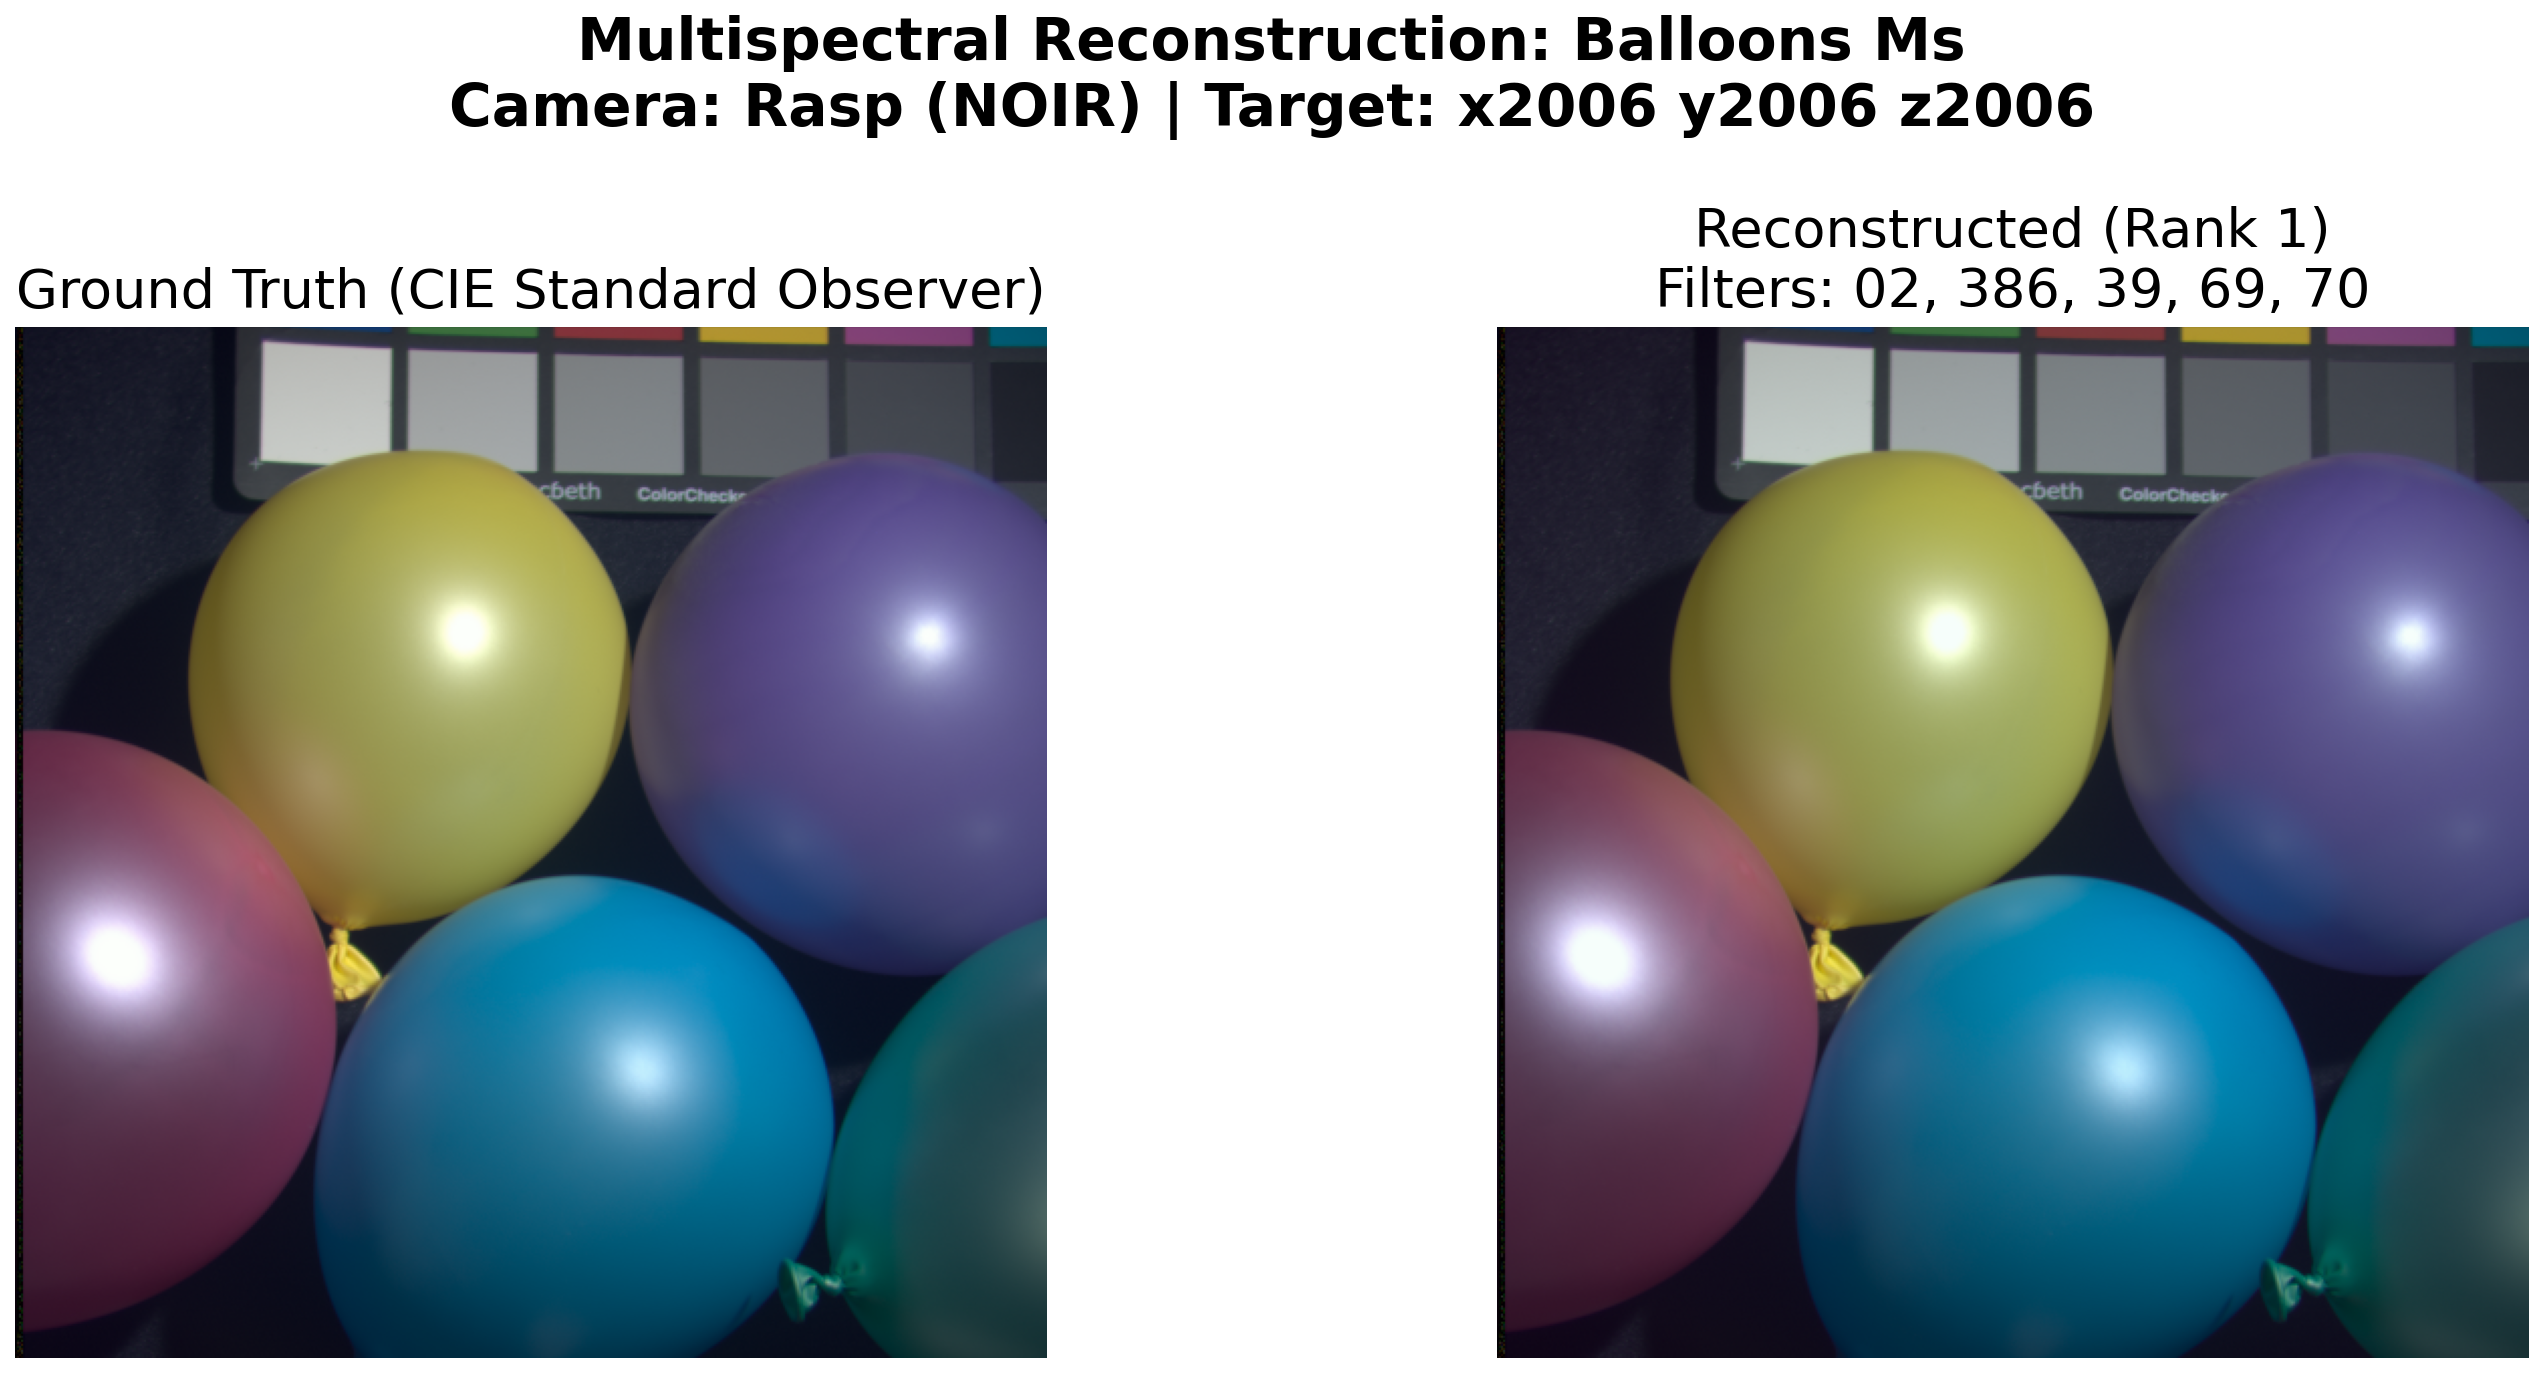
\includegraphics[width=\linewidth]{media/measured_k5_cave.png}
    \caption{CAVE dataset rendering}
\end{subfigure}
\caption{Supergel results for $k=5$.}
\label{fig:k5spectral}
\end{figure}


\begin{figure}[H]
\centering
\begin{subfigure}{.40\linewidth}
    \centering
    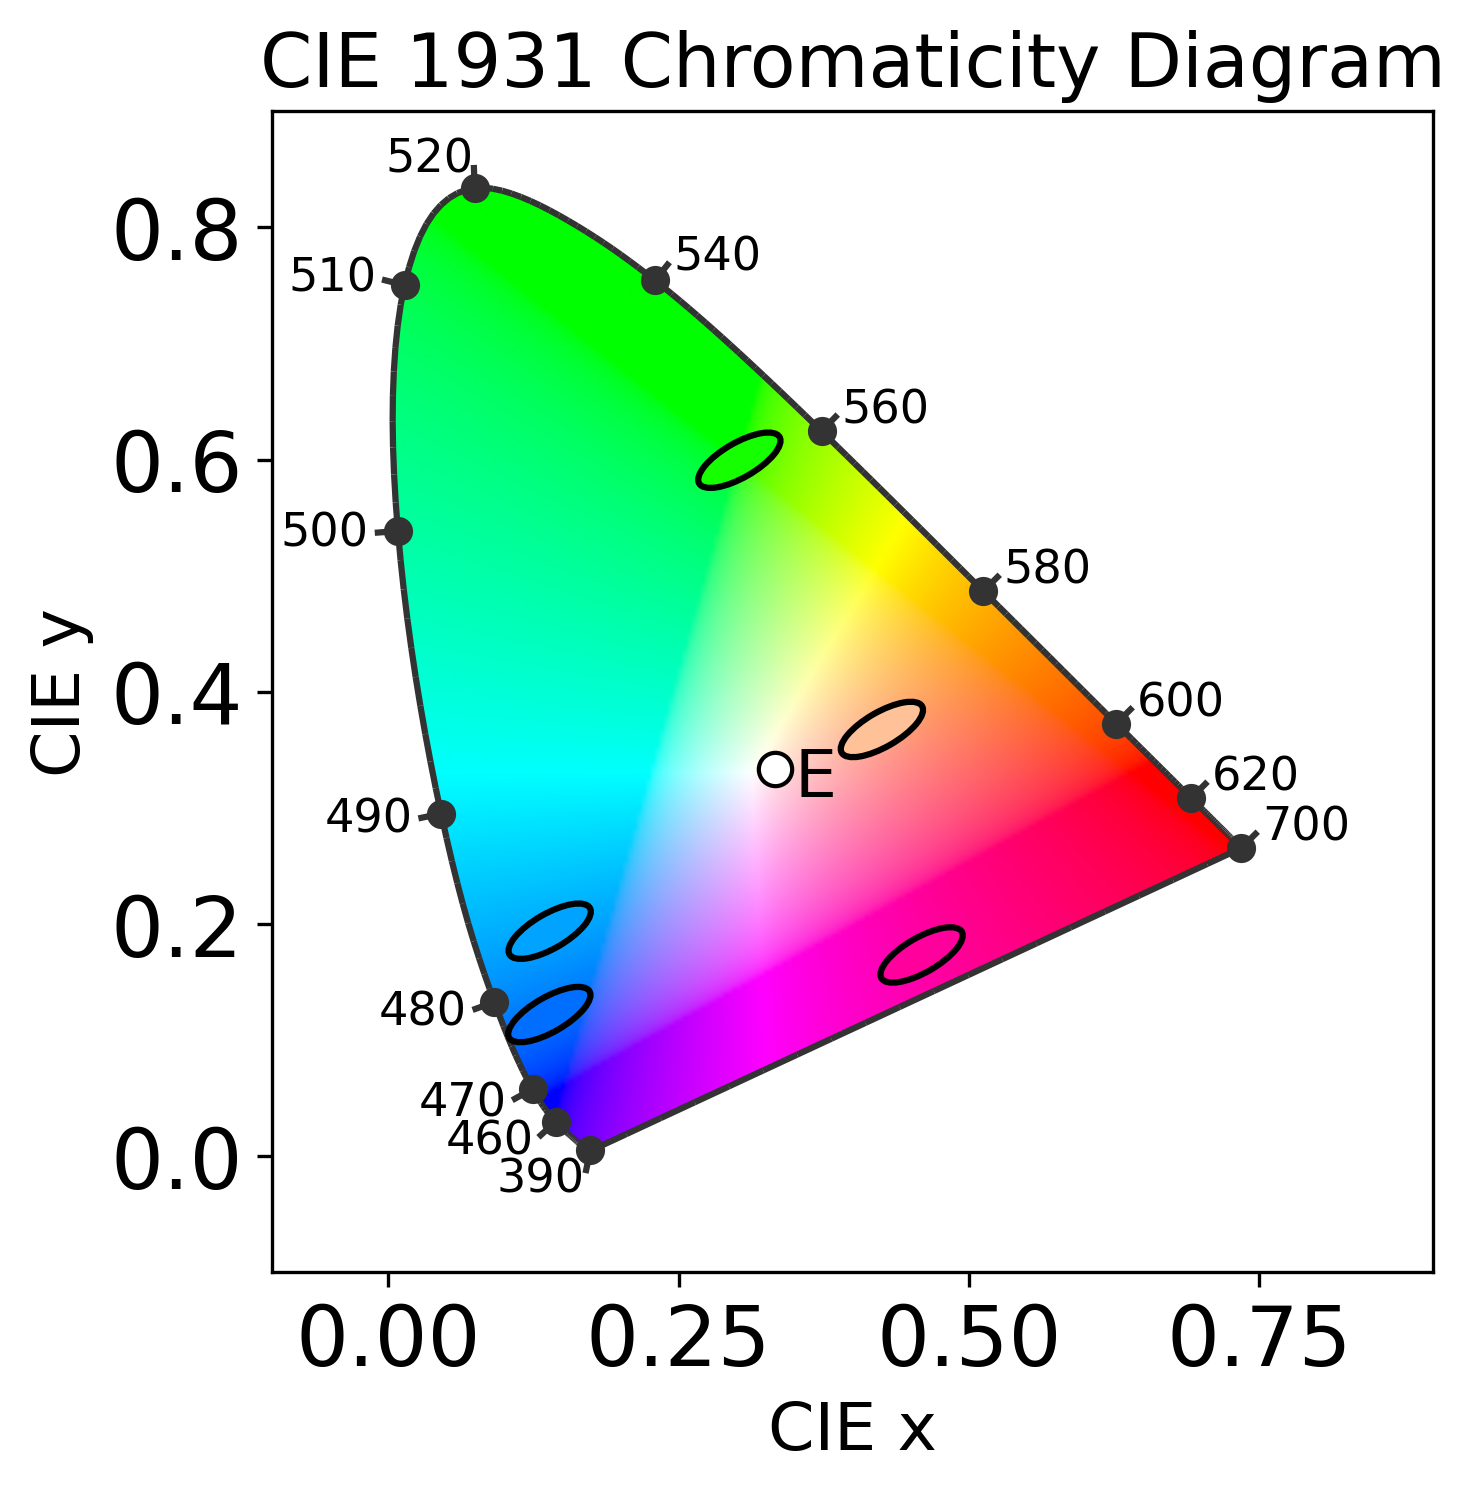
\includegraphics[width=\linewidth]{media/measured_k5_gamut.png}
    \caption{Location on CIE 1931 Color Gamut}
\end{subfigure}%
\begin{subfigure}{.55\linewidth}
    \centering
    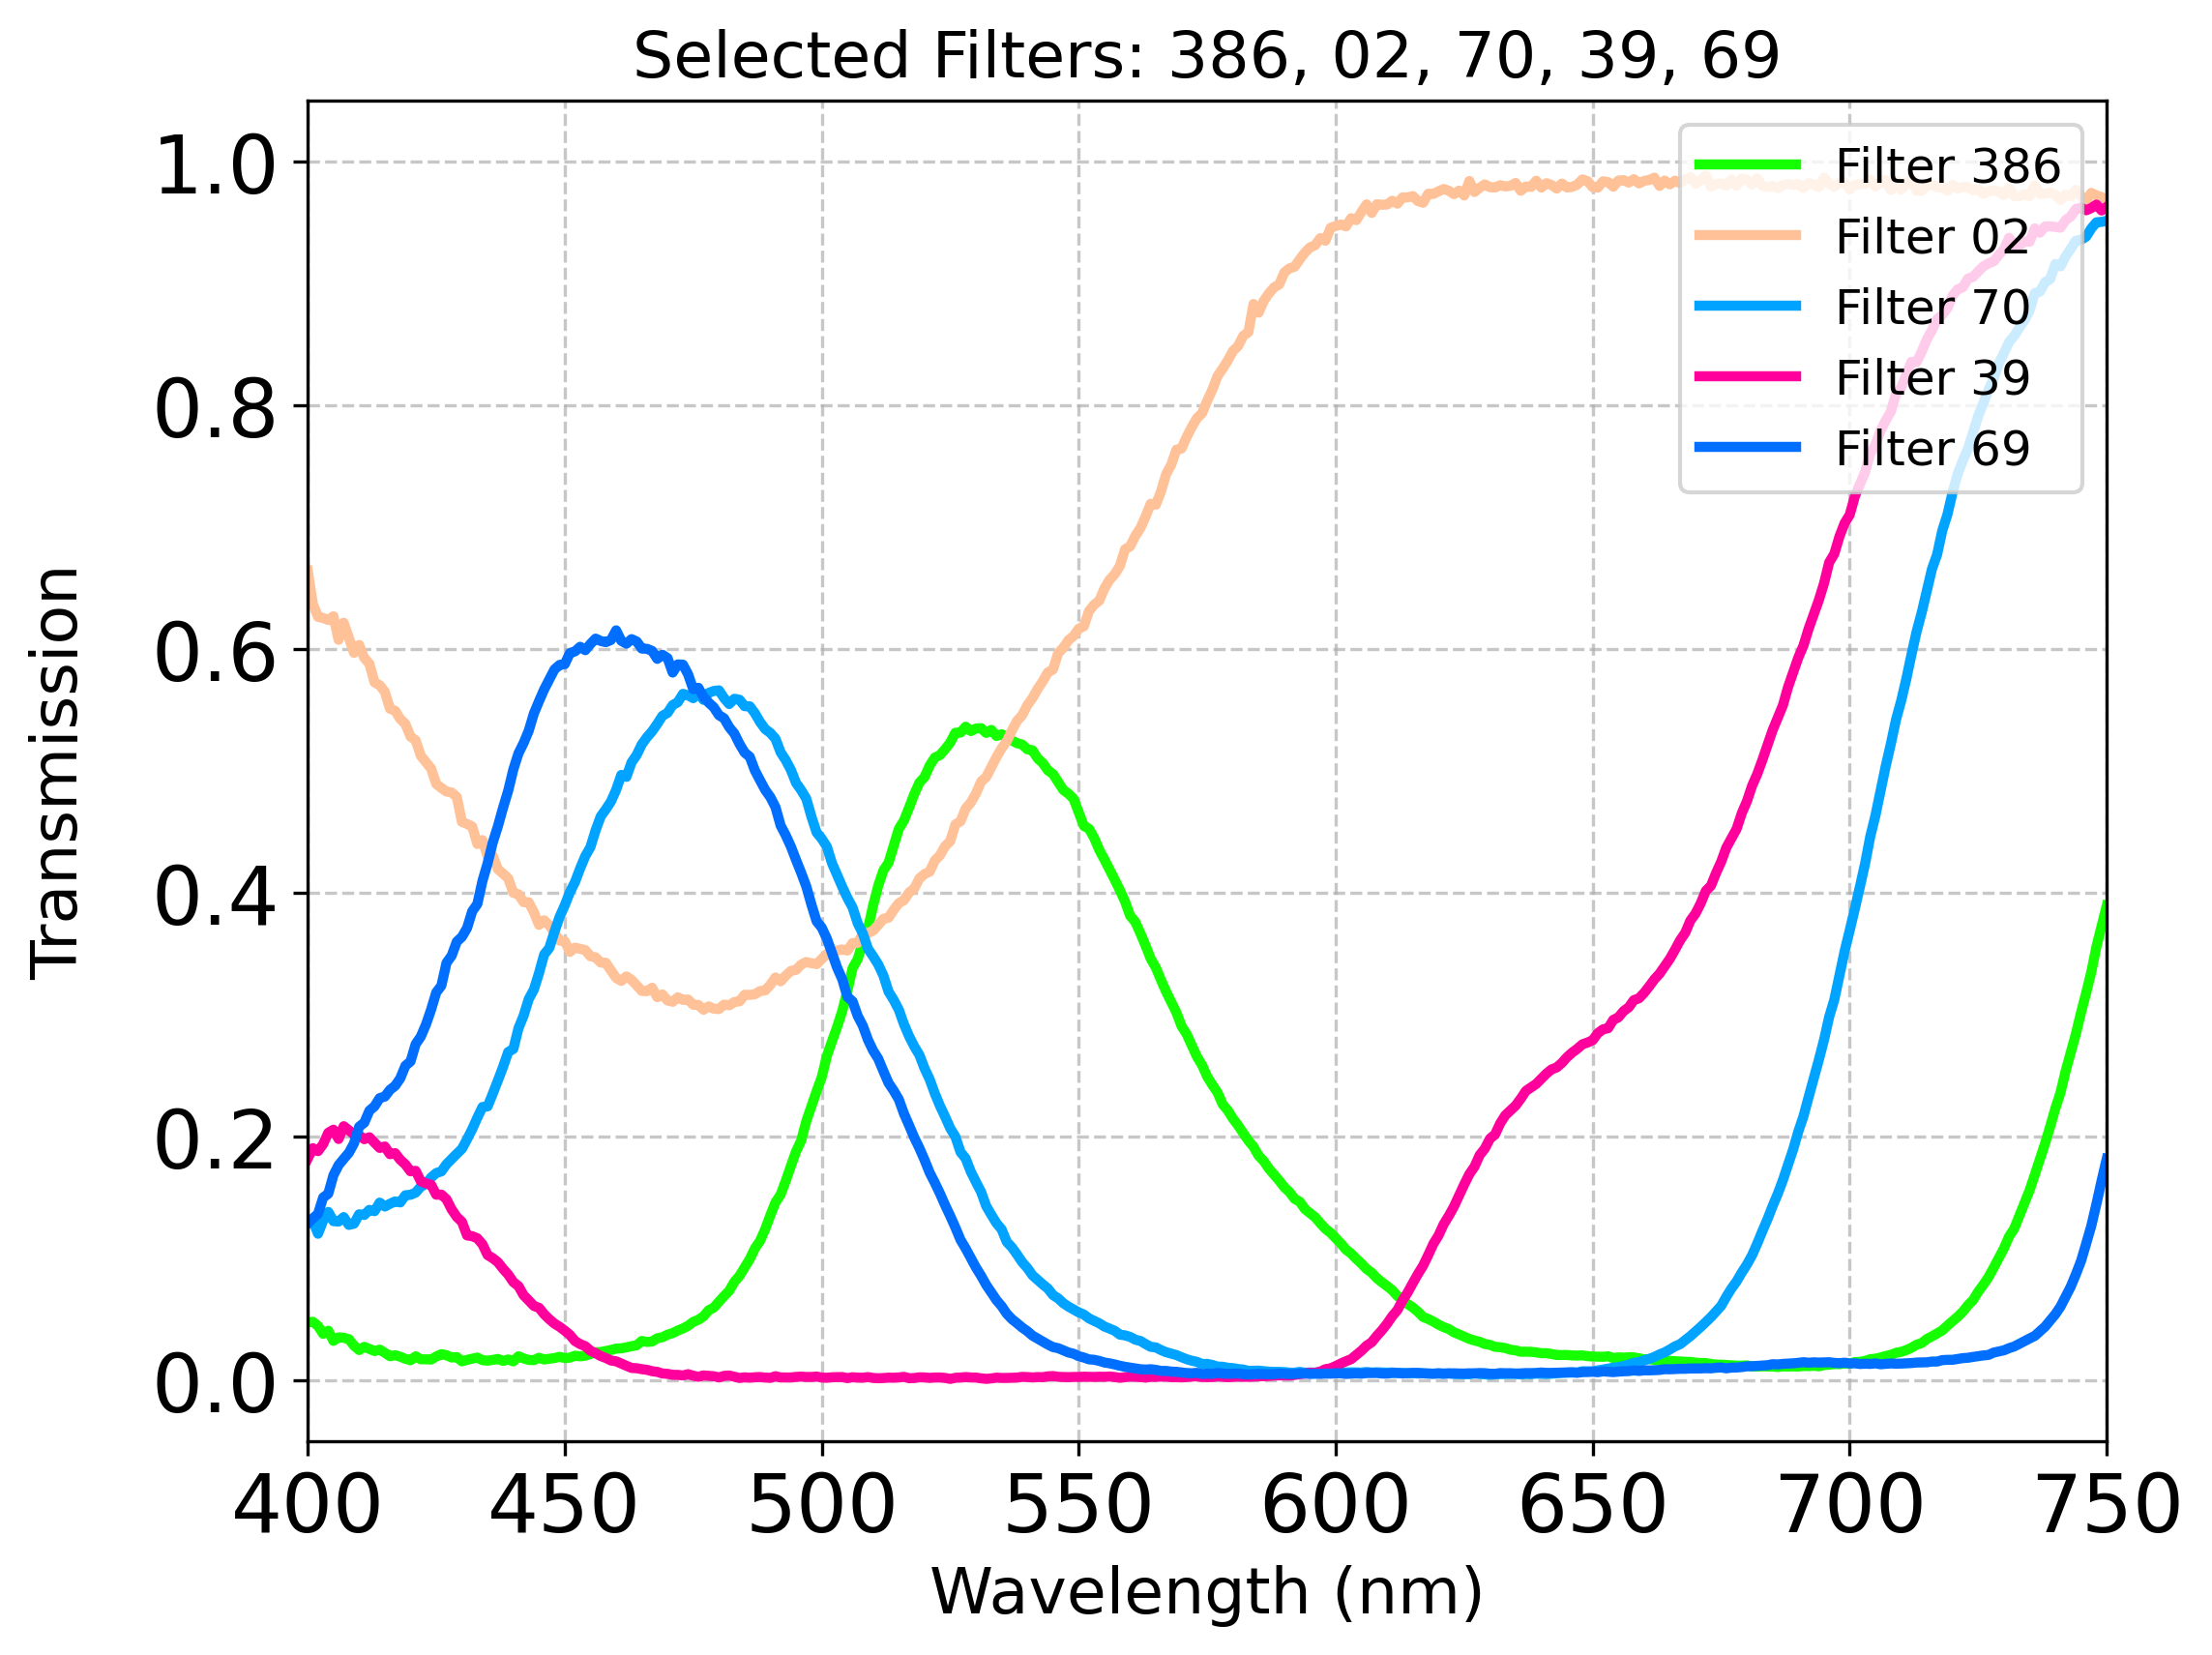
\includegraphics[width=\linewidth]{media/measured_k5_transmission.png}
    \caption{Transmission functions of selected filters}
\end{subfigure}
\caption{$k=5$ Transmission functions and location on gamut}
\label{fig:k5Transmissions}
\end{figure}

Additional captures from the CAVE dataset are included in the appendix. 

\subsection{CIE 2006 10-degree CMF}

We focus our prior research on the 2-degree CMF derived by Stockman \& Sharpe \cite{STOCKMAN20001711}, but also show that with minimal overhead, we can provide an effective filter selection for the 10 degree color matching functions enumerated in the same body of research. 
In this context, the 'degree' refers to the field of view of the observer.
While we only achieve $\dE<1$ at $k=6$, this is a reasonable result. 
We note that the original PCA algorithm performs worse than the PCA2 algorithm (Algorithm 3), the former failing to find a selection which identifies a combination with $\dE<1$.

\begin{figure}[H]
\centering
\begin{subfigure}{.64\linewidth}
    \centering
    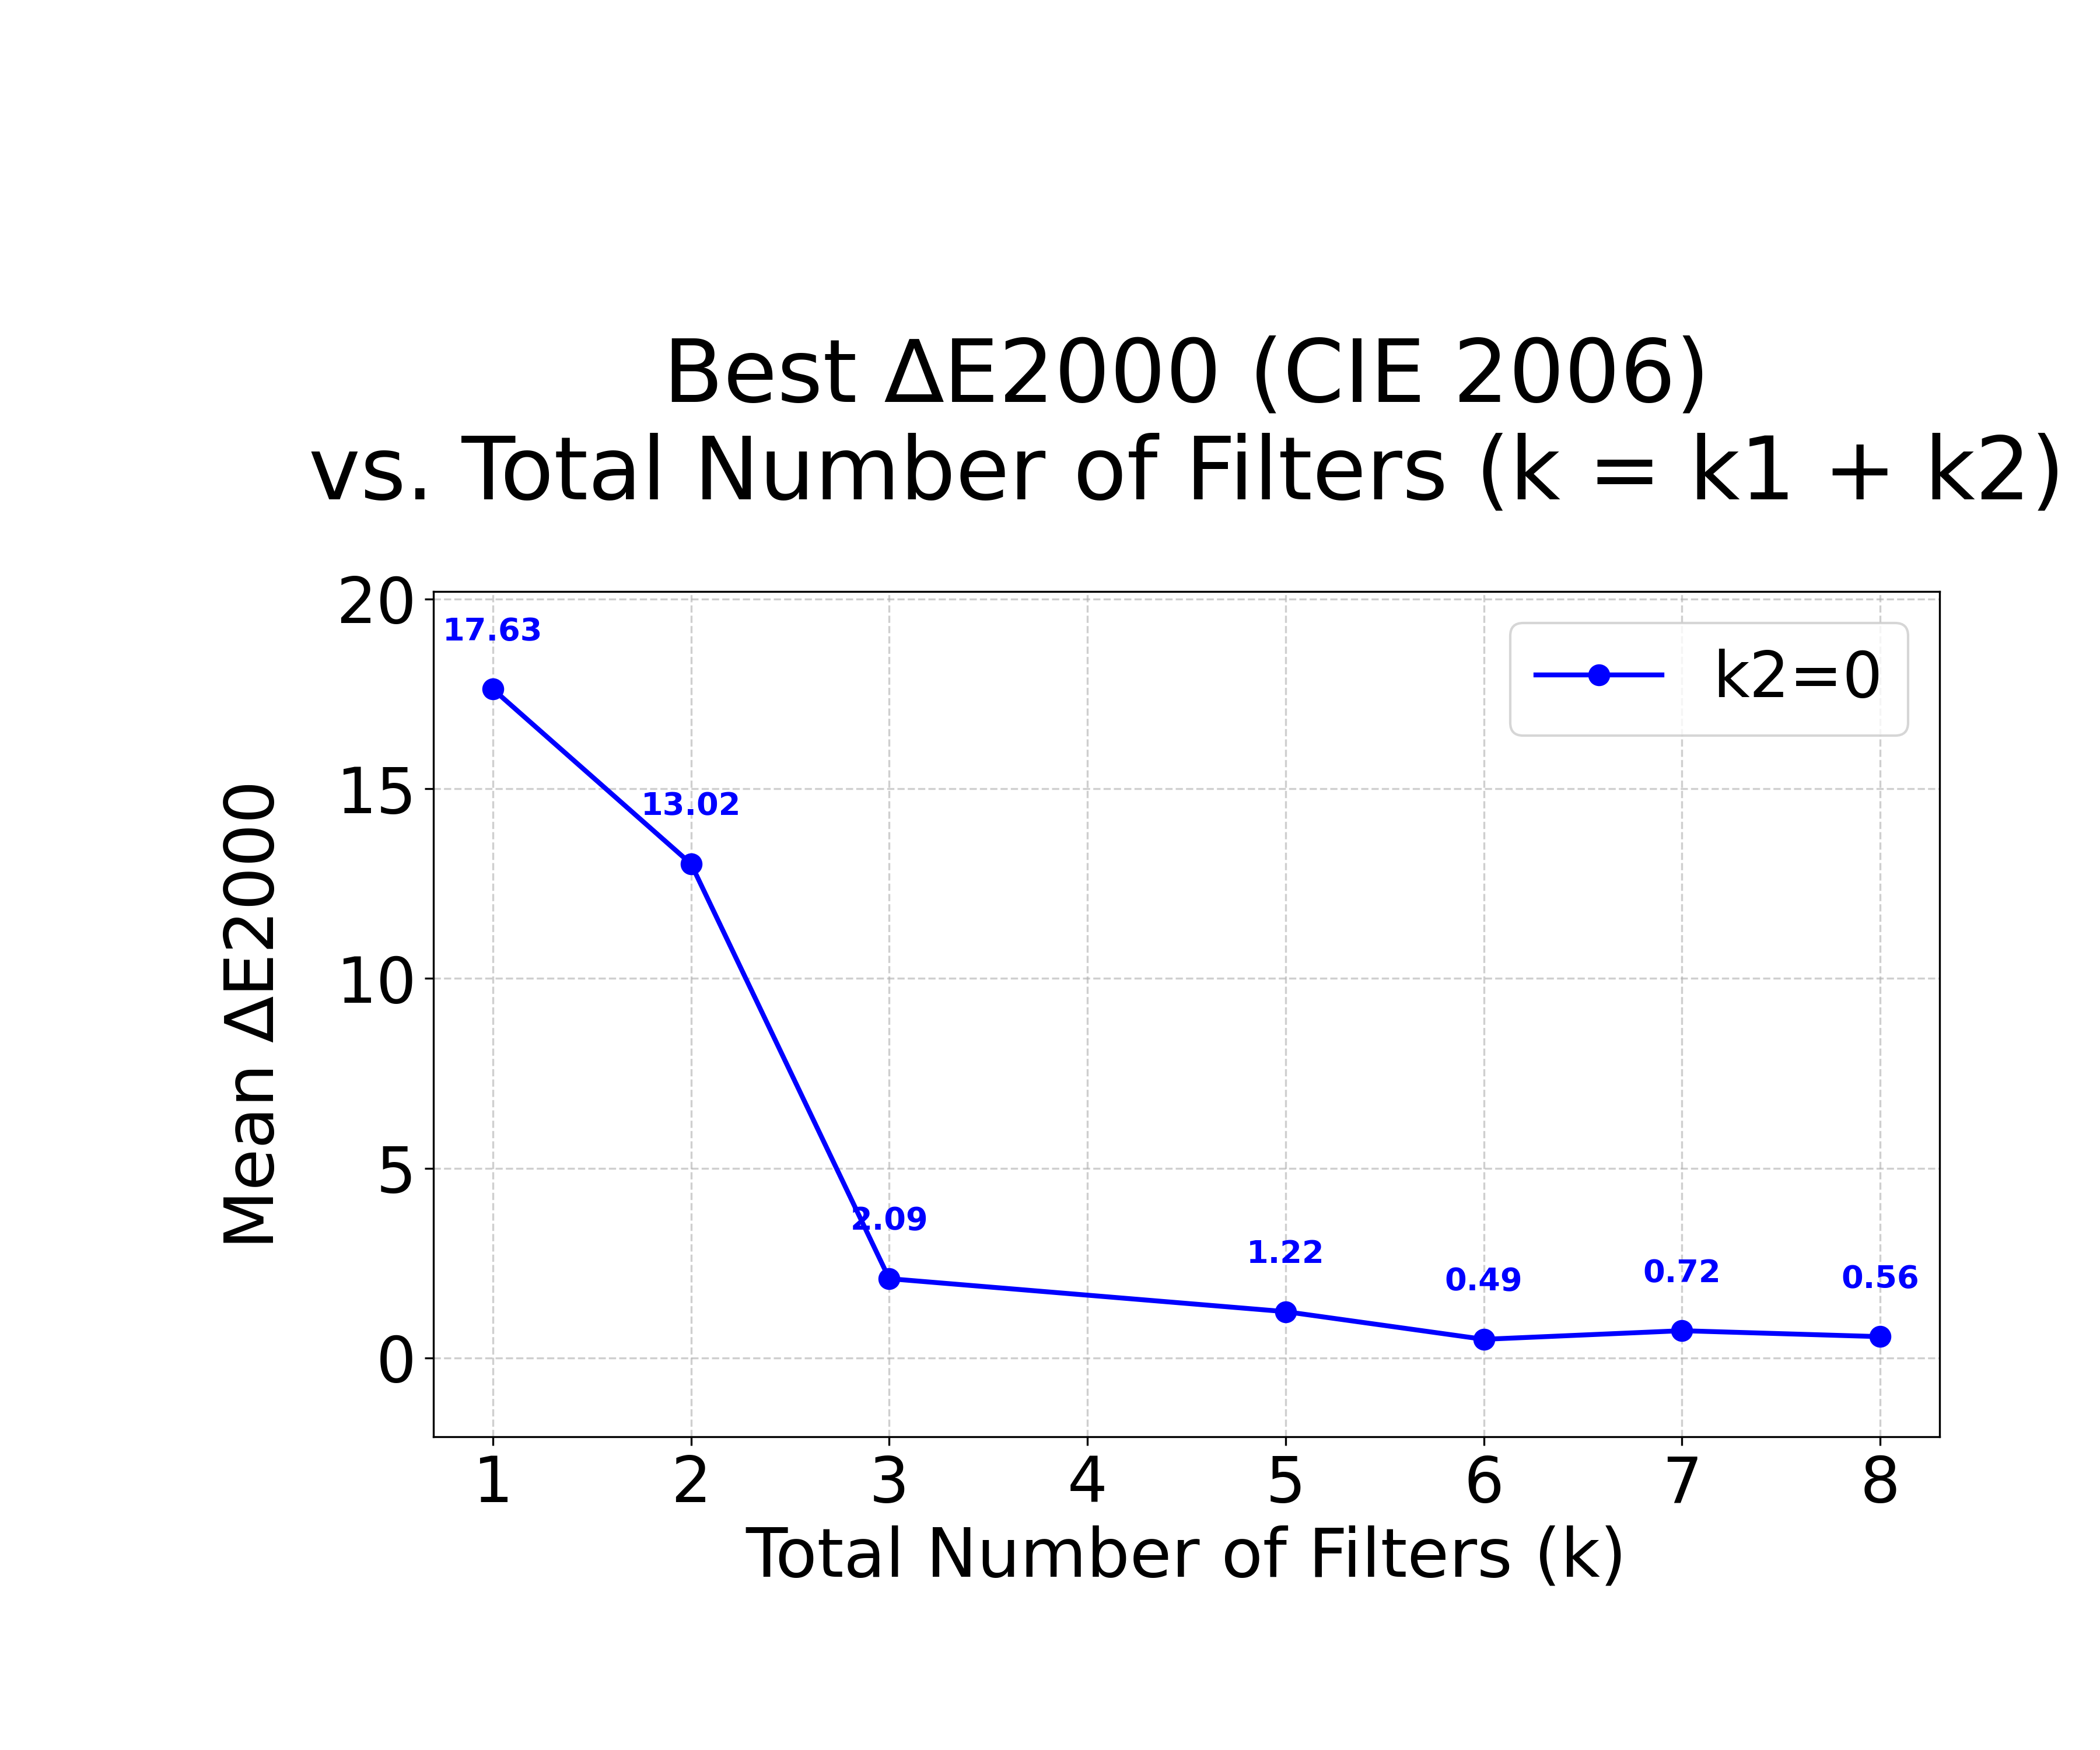
\includegraphics[width=.55\linewidth]{media/deltaE_vs_k_mse10d.png}
    \caption{$\dE$ for $k \in \{1,2...8\}$ for the 10 degree observer}
\end{subfigure}%
\begin{subfigure}{.34\linewidth}
    \centering
    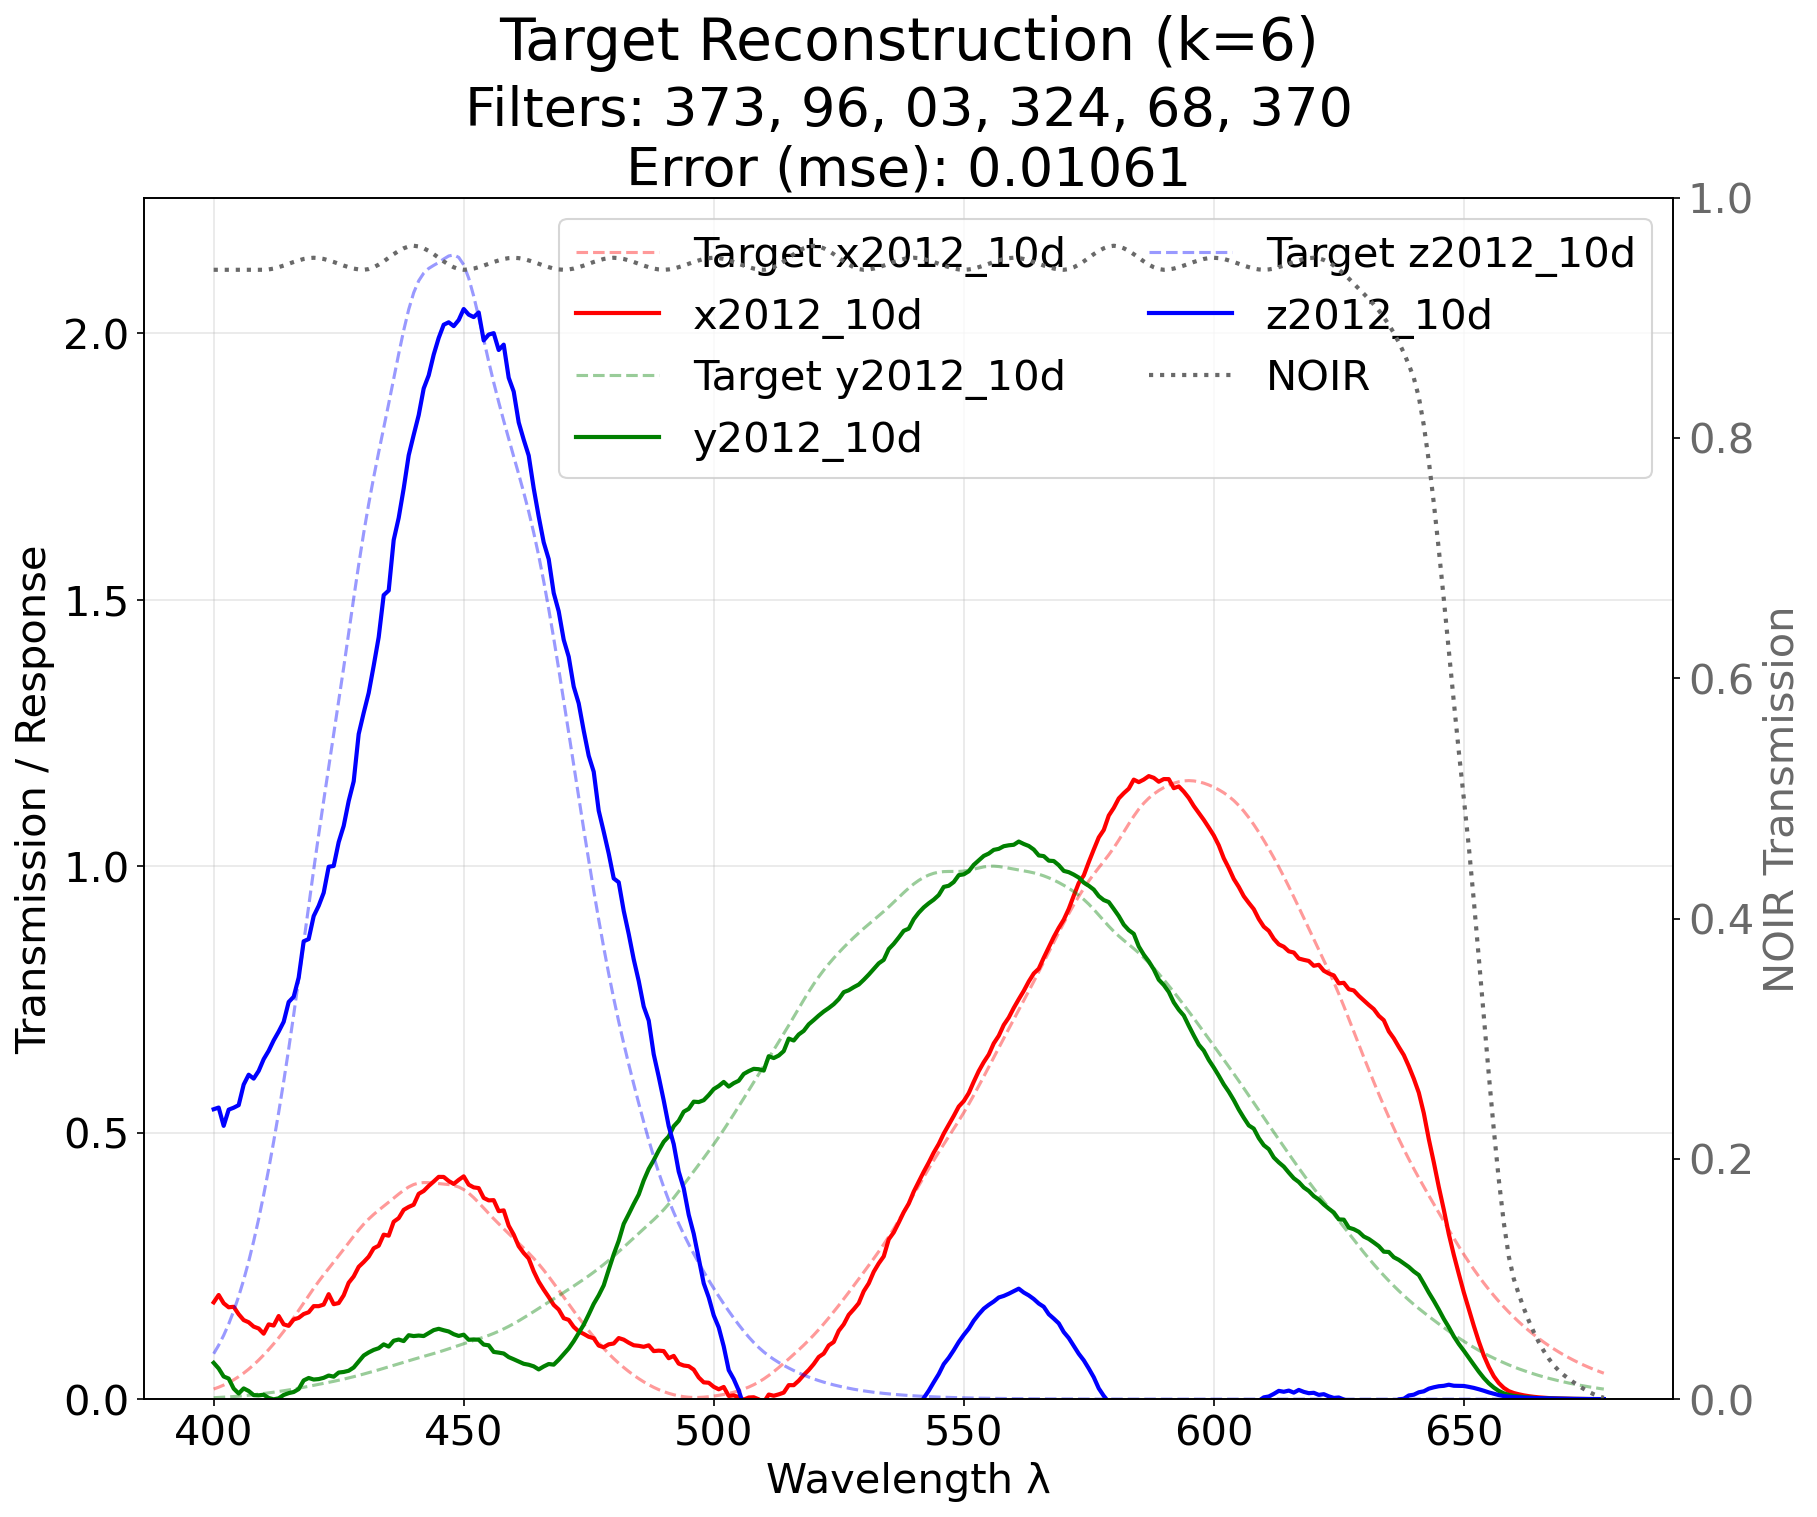
\includegraphics[width=\linewidth]{media/top1_spectra_10d.png}
    \caption{Best Spectral Reconstruction}
\end{subfigure}
\caption{Lab setup for image capture, with deconstructed camera}
\label{fig:10Degrees}
\end{figure}

\section{Algorithm Comparison}

In this section, we analyze the best MSE and $\dE$ for the brute force and PCA algorithms, in the simulated Rosco Supergel set. 
We see that counterintuitively, the best $\dE$ performances are found at the $k_1=3$ and $k_1=4$, $k_2=2$ filter selectors. 
Additionally, we note that the performance is not monotonically decreasing due to the difficulties of the filter selection problem, but again, these $\dE$ metrics are below the just noticeable difference of 1, and thus we note that the simulated reconstructions are fairly indistinguishable from ground truth. 

\begin{table}[H]
    \centering
    \begin{tabular}{llrrrr}
    \toprule
     &  & \multicolumn{2}{r}{Best MSE} & \multicolumn{2}{r}{Best $\dE$} \\
     & Strategy & Brute Force & PCA & Brute Force & PCA \\
    N & N2 &  &  &  &  \\
    \midrule
    \multirow[t]{3}{*}{1} & 0 & 0.1904 & 0.2003 & 20.8603 & 17.7365 \\
      & 1 & 0.1432 & 0.0500 & 12.7010 & 12.6795 \\
      & 2 & 0.0263 & 0.0205 & 7.9875 & 4.6905 \\
    \cline{1-6}
    \multirow[t]{3}{*}{2} & 0 & 0.0489 & 0.0791 & 13.1686 & 13.5027 \\
      & 1 & 0.0392 & 0.0272 & 9.8836 & 6.9481 \\
      & 2 & 0.0188 & 0.0117 & 1.1743 & 1.8973 \\
    \cline{1-6}
    \multirow[t]{3}{*}{3} & 0 & 0.0219 & 0.0457 & 5.4475 & 2.8156 \\
      & 1 & 0.0220 & 0.0117 & 5.3174 & 1.8973 \\
      & 2 & 0.0089 & 0.0037 & 1.5786 & 0.5551 \\
    \cline{1-6}
    \multirow[t]{3}{*}{4} & 0 & 0.0063 & 0.0318 & 1.9277 & 1.6631 \\
      & 1 & 0.0229 & 0.0062 & 1.7381 & 0.9180 \\
      & 2 & 0.0033 & 0.0025 & 0.5718 & 0.3909 \\
    \cline{1-6}
    \multirow[t]{3}{*}{5} & 0 & 0.0034 & 0.0197 & 0.9064 & 0.5701 \\
      & 1 & 0.0108 & 0.0047 & 4.7085 & 0.7234 \\
      & 2 & 0.0021 & 0.0018 & 0.5258 & 0.4879 \\
    \cline{1-6}
    \multirow[t]{3}{*}{6} & 0 & 0.0021 & 0.0146 & 0.4550 & 0.6770 \\
      & 1 & 0.0033 & 0.0044 & 0.6592 & 0.6900 \\
      & 2 & 0.0018 & 0.0015 & 0.4961 & 0.4676 \\
    \cline{1-6}
    \bottomrule
    \end{tabular}
    \caption{Minimum MSE and $\Delta E$ Comparison: PCA vs. Brute Force}
    \label{tab:mse_deltae_comparison}
\end{table}


\subsection{Noise Model Analysis}

For analysis of the noisiness of our capture, we switch from the MSE loss function to the MSE_noisy loss function, and we compare the results with increments in the photons parameter. 
For this analysis, we increment along the $k_1$ parameter amongst $k_1 \in \{2,4,6\}$, fixing $k_2=2$. 
The difference in $\dE$ performance using the noise model is significantly larger due to the worse reconstruction quality attained by adding noise to the loss function.
Hence, $\dE$ attained with $k=4 (k_1=2,k_2=2)$ filters never decreases past 14. 

\begin{center}
    \centering
    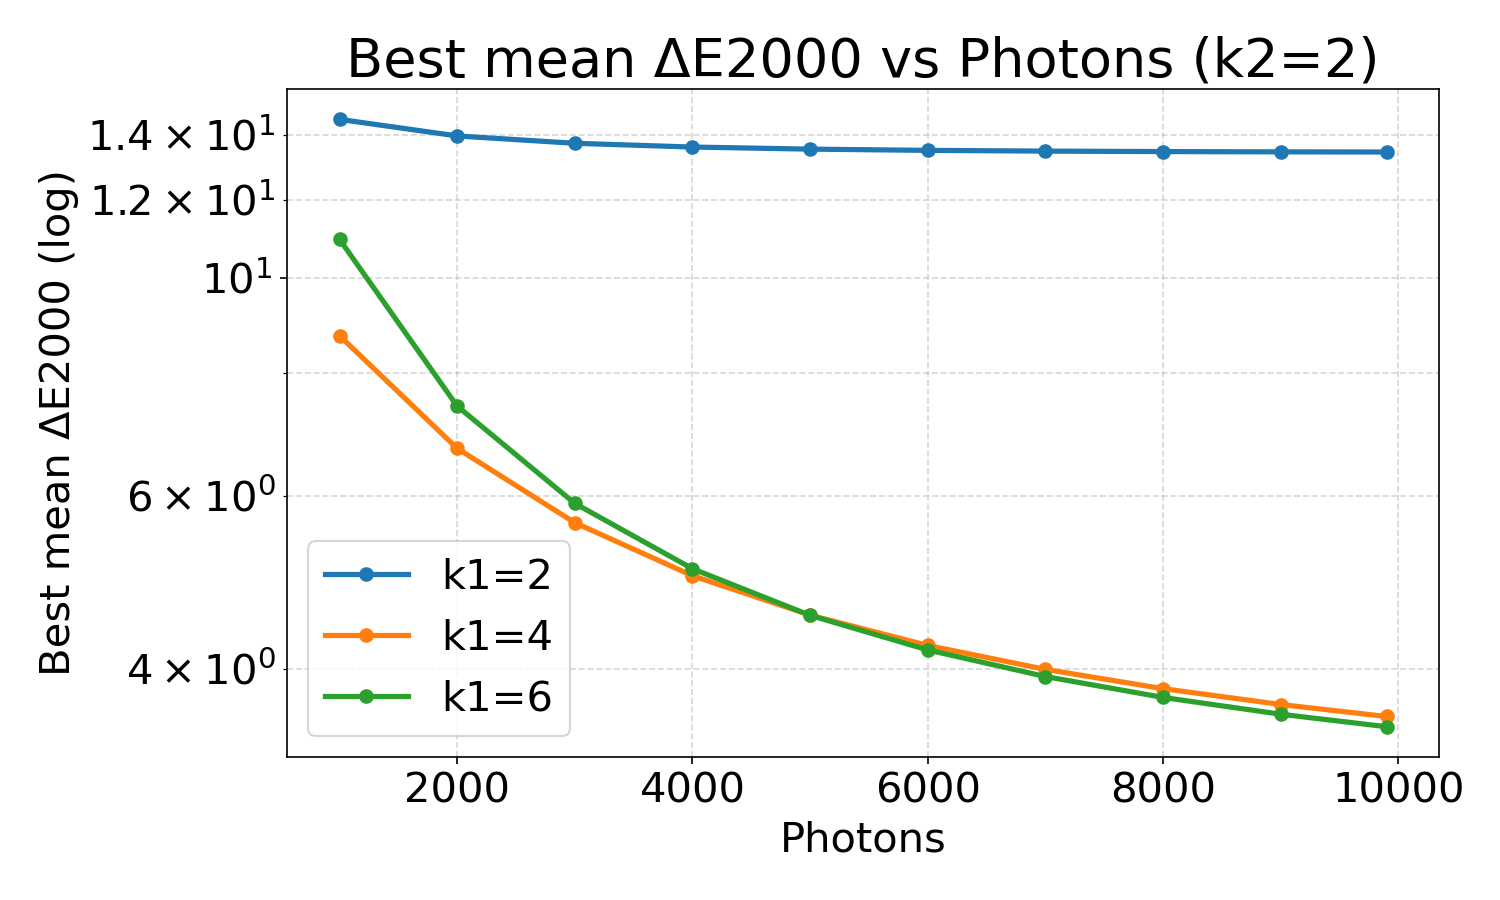
\includegraphics[width=.75\linewidth]{media/photons_sweep_deltaE_20260528_210811.png}
    \captionof{figure}{Best $\dE$ as a function of Photons}
\end{center}

The noise model is not directly used in our filter selection process, but informs our understanding of filter wheel dynamics and shutter speed. 
We also recognize the detrimental effect of poor lighting on our captures, and aim to increase exposure time in low-lighting environments.


\section{Physical Camera with Rosco Supergel Set}

For the initial evaluation of our physical camera stack, we stage an environment under the same Lilliput \cite{UtopiaCamLiliput} illuminant in a lab environment. 
We position the illuminant about 2 meters above the scene to tune the intensity of light into the camera aperture, and place our camera (removed from the housing) on a tripod, aimed at the stage. 

\begin{center}

\end{center}

\begin{figure}[H]
\centering
\begin{subfigure}{.64\linewidth}
    \centering
    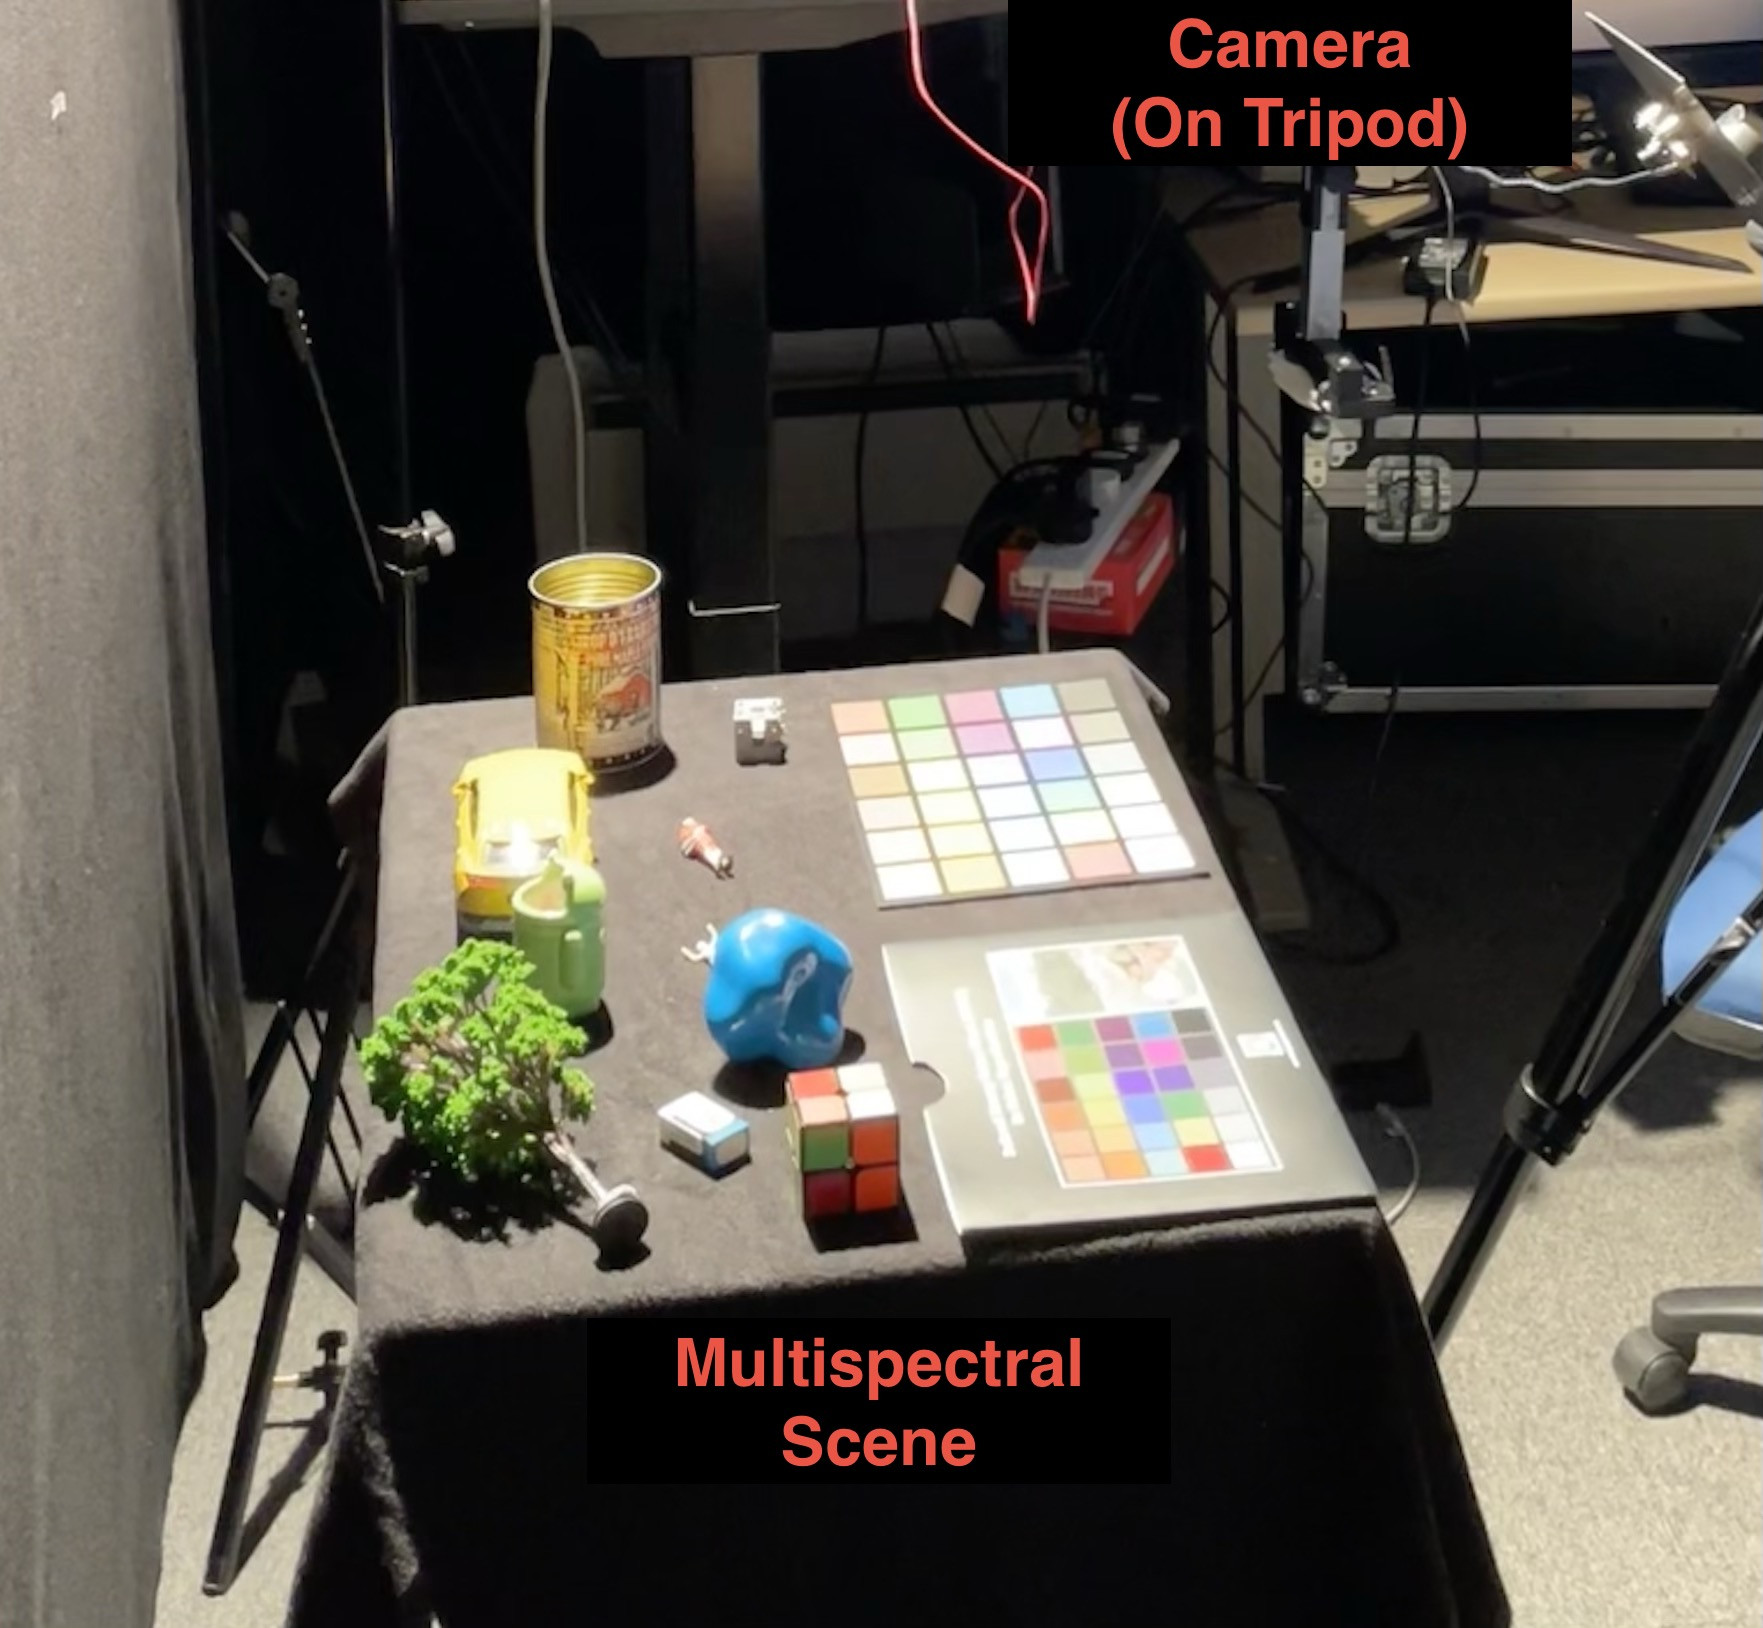
\includegraphics[width=.55\linewidth]{media/spectralLabMarkup.jpeg}
    \caption{Camera on tripod in lab, side angle}
\end{subfigure}%
\begin{subfigure}{.34\linewidth}
    \centering
    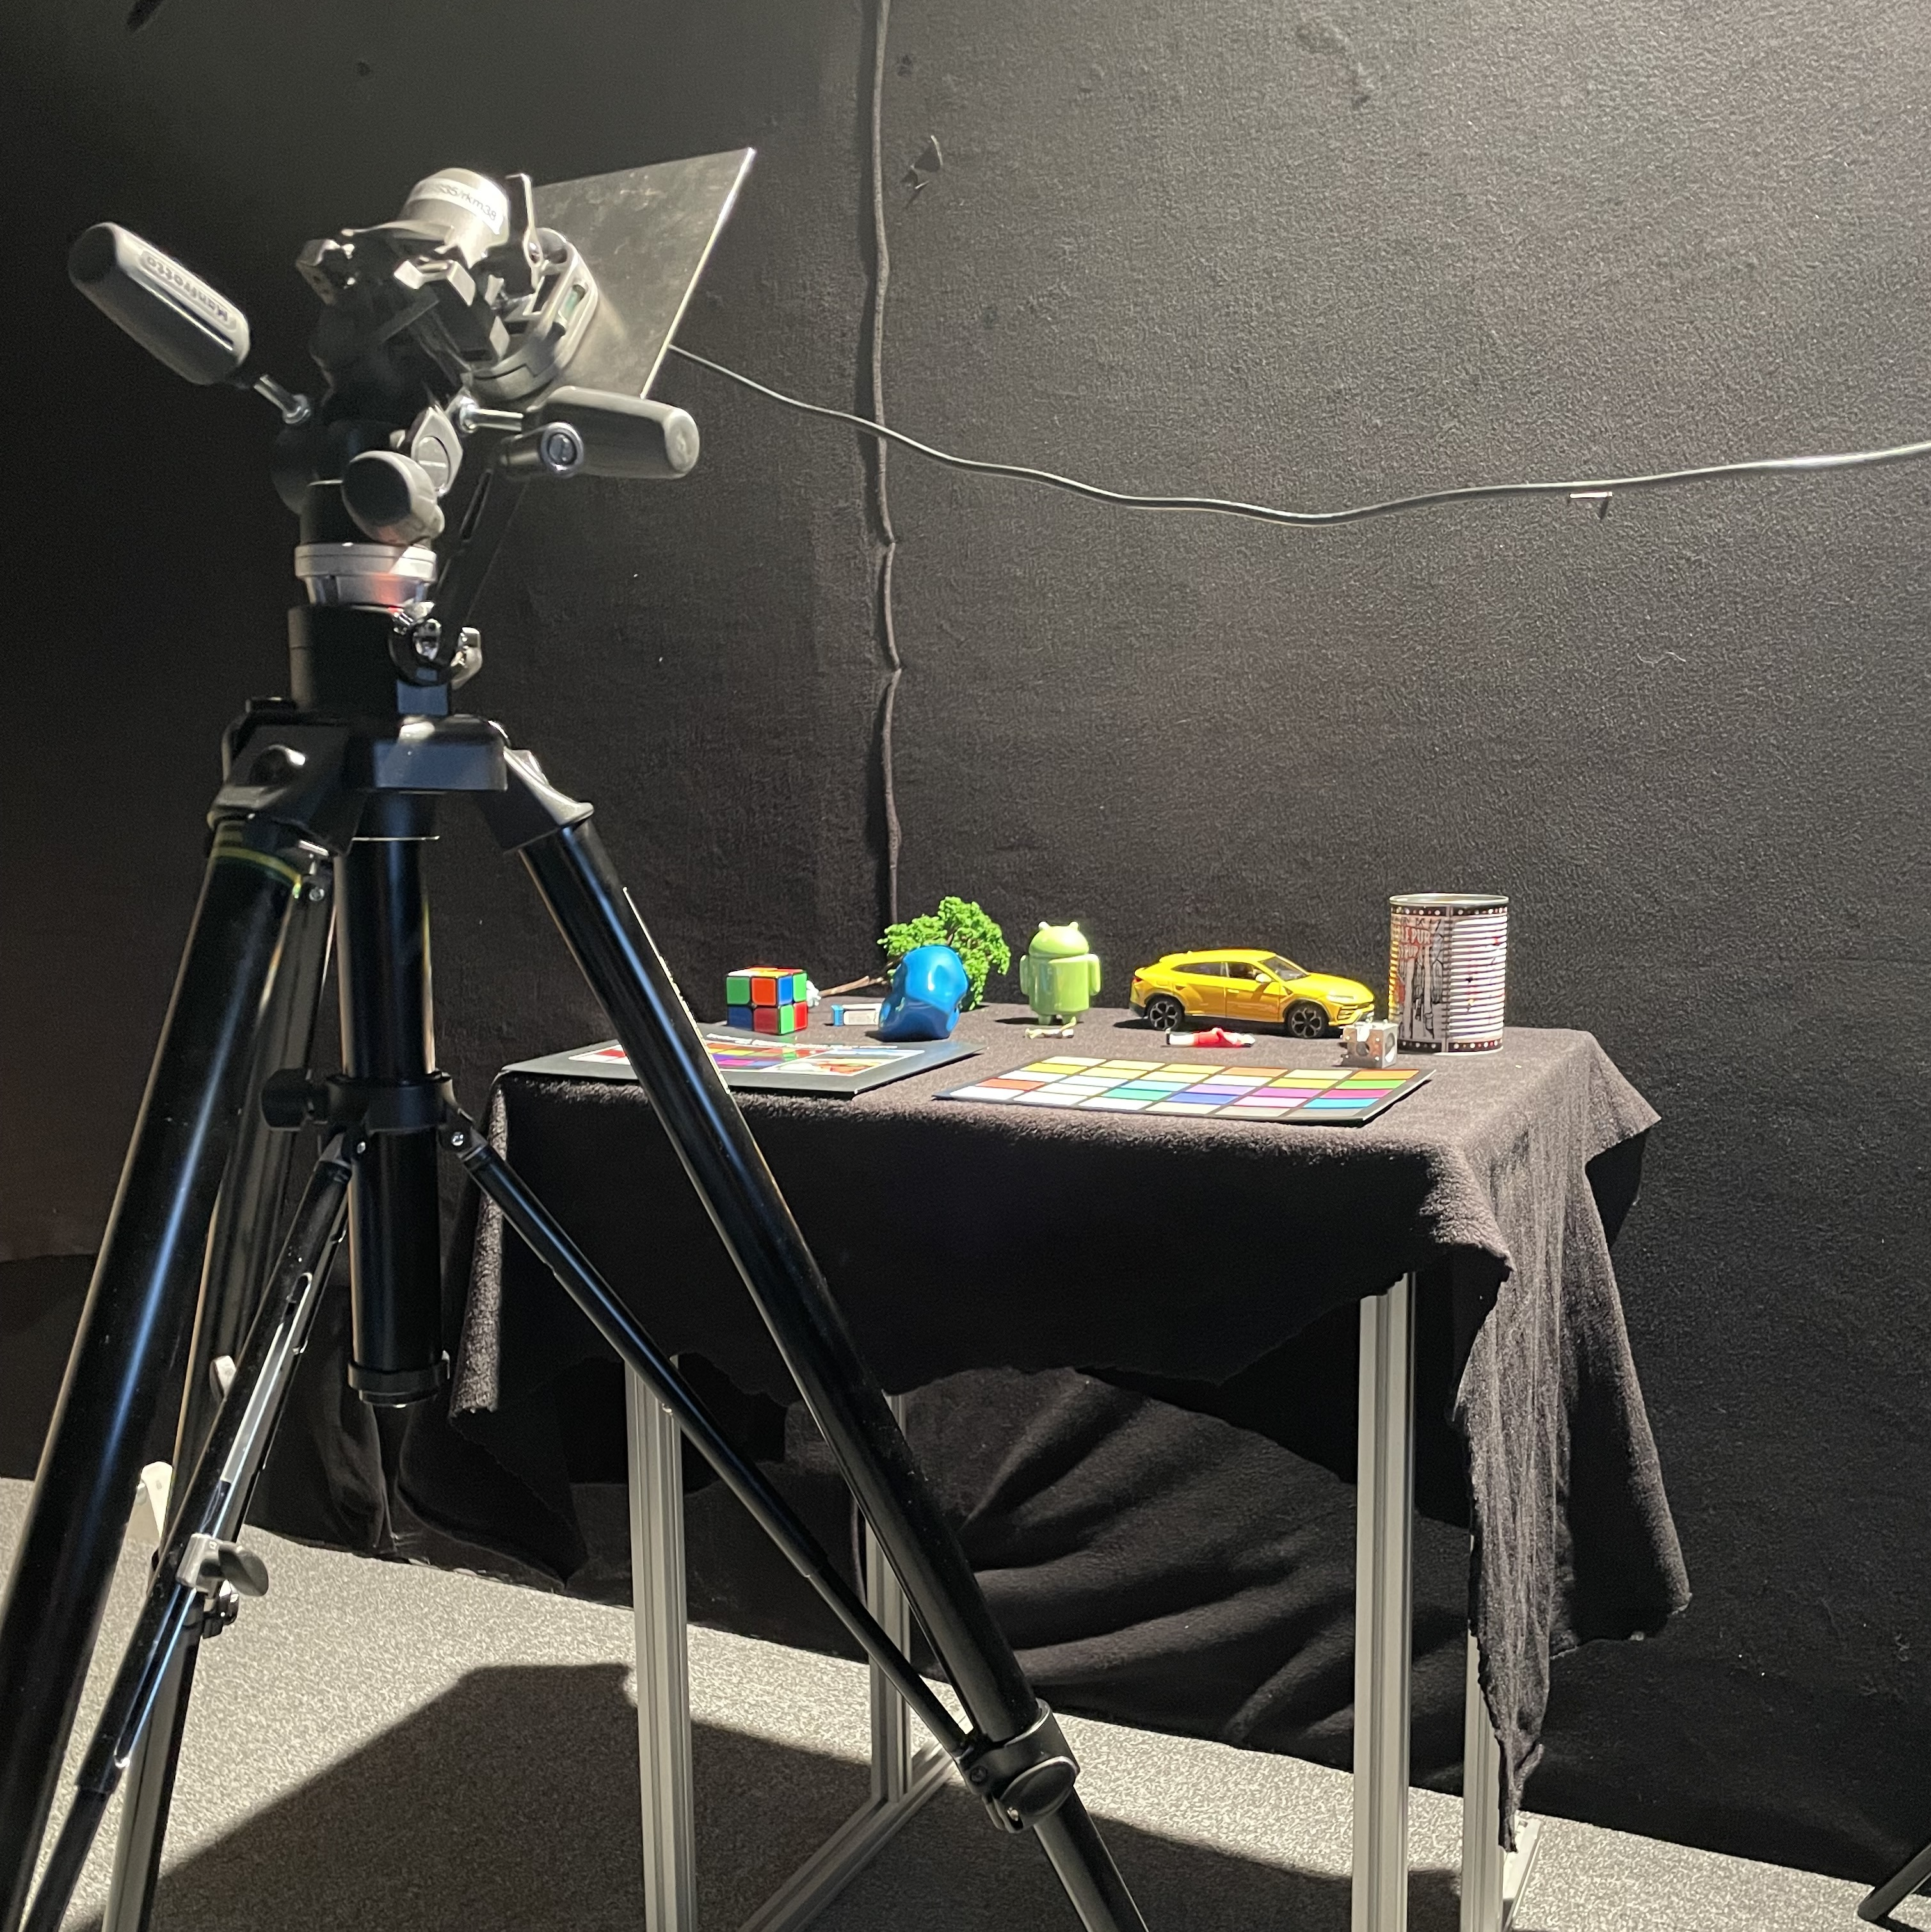
\includegraphics[width=\linewidth]{media/spectralLabMarkupStage.jpeg}
    \caption{Camera on tripod, rear angle}
\end{subfigure}
\caption{Lab setup for image capture, with deconstructed camera}
\label{fig:spectralLabMark}
\end{figure}

Then, we test the recommended best performing filter combinations against a multispectral scene including a PMC in a lab environment, using the Rosco Supergel set of filters. 

We then take the best prescribed reconstructions for the $k_1=4$ and $k_1=5$ reconstructions to test our methodology. 

\begin{center}
    \centering
    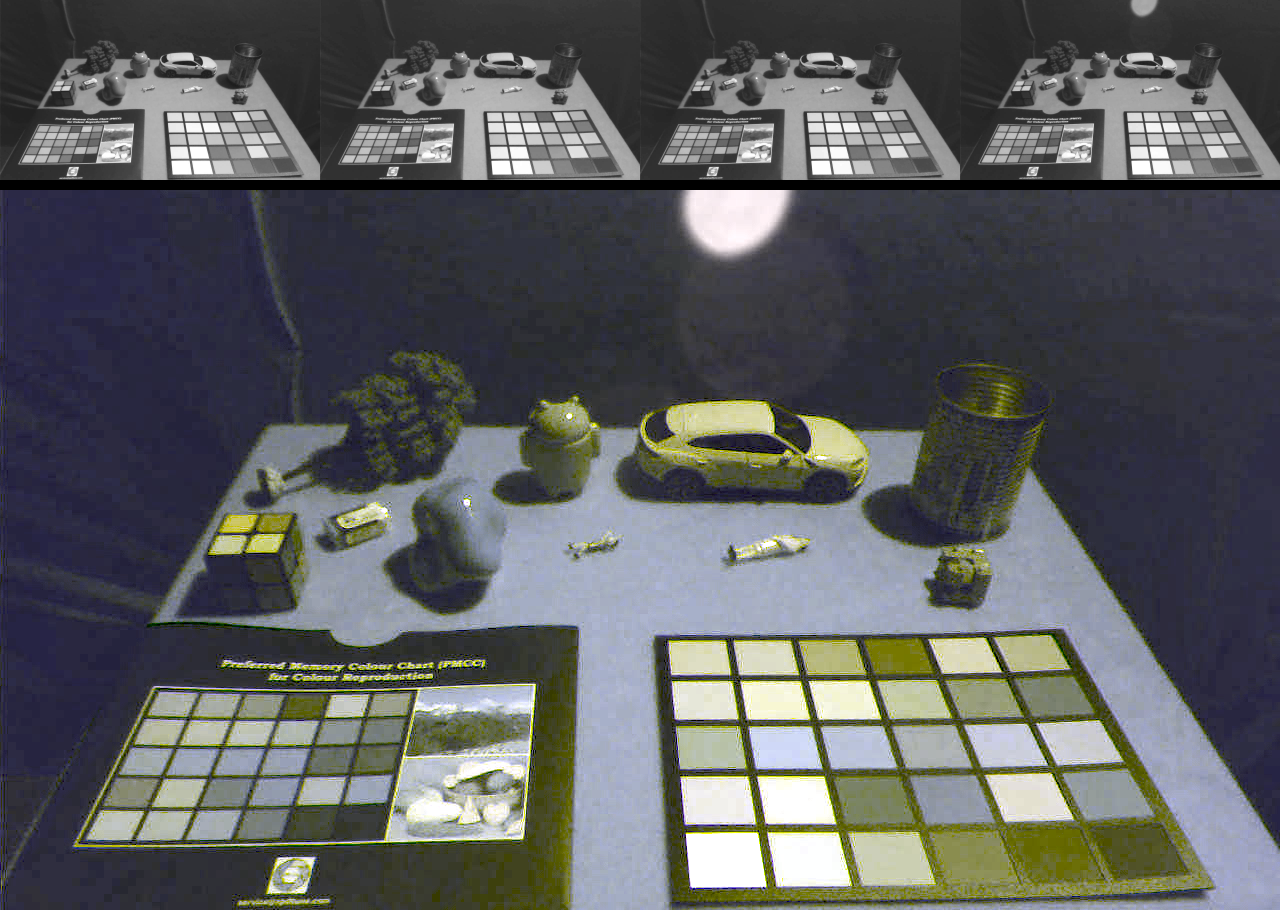
\includegraphics[width=.75\linewidth]{media/k1_4_recon.png}
    \captionof{figure}{$k_1=4$ Photo Lab Reconstruction with component captures above}
\end{center}

Qualitatively, we see that these solutions do not provide perfect reconstructions, and the intensity of some of the hues is dulled. 
For a more quantitative analysis, we utilize the spectrophotometer in this same lab environment \ref{ref:spectrophotometer} and compute the ground truth $x$ and $y$ values. 
Then, we can use the same methodology as the simulated pipeline to compute $\dE$. 

Here, we have the solution for the $k_1=5$ 

\begin{center}
    \centering
    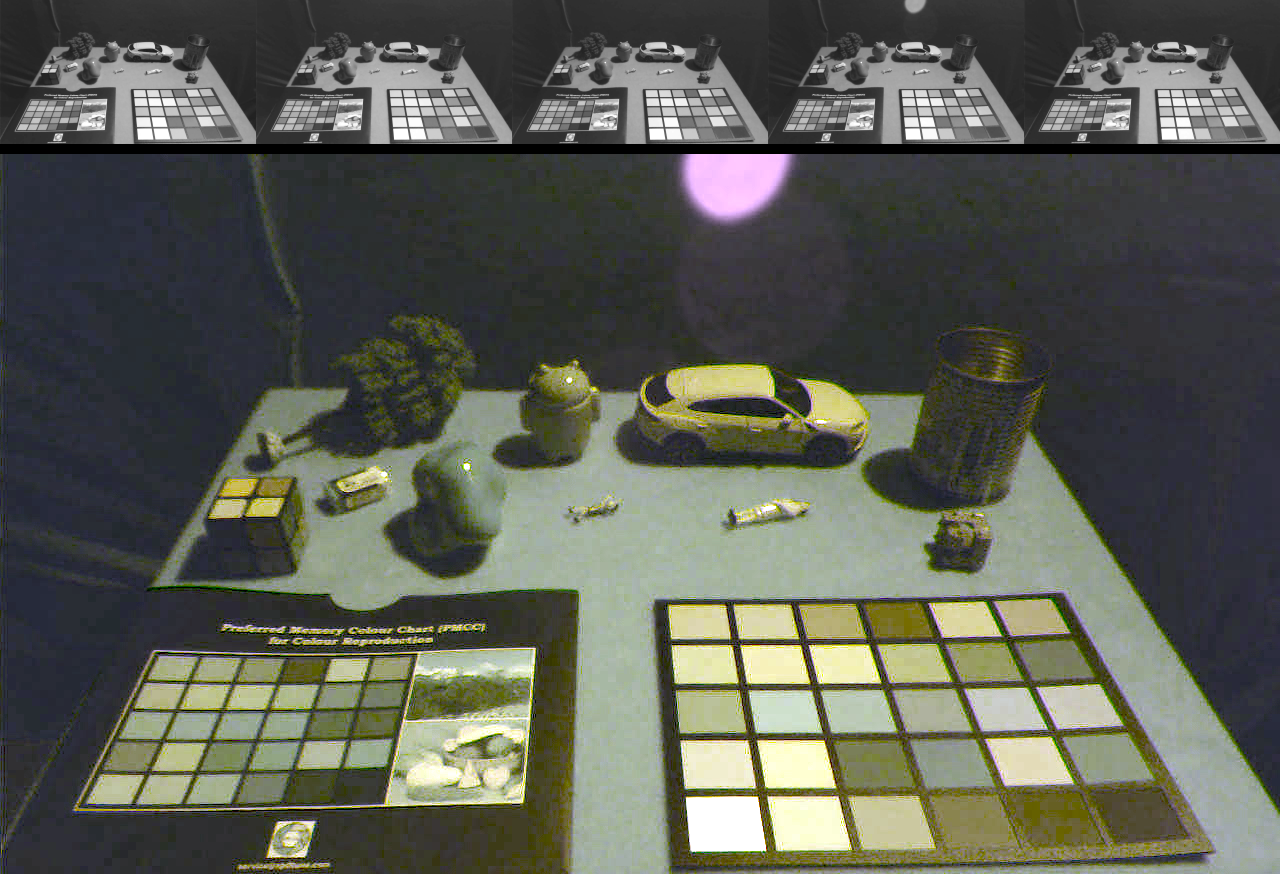
\includegraphics[width=.75\linewidth]{media/k1_5_recon.png}
    \captionof{figure}{$k_1=5$ Photo Lab Reconstruction with component captures above}
\end{center}

\iffalse
\section{Physical Camera Photo Results}

We demonstrate use of our physical camera in non-laboratory settings. 
Here, we have a photo of ____, reconstructed with a filter wheel 
\begin{figure}[H]
\centering
\begin{subfigure}{.49\linewidth}
    \centering
    
\includegraphics[width=\linewidth]{media/placeholder.jpg}
    \caption{Camera and subject taking image of ____}
\end{subfigure}
\begin{subfigure}{.49\linewidth}
    \centering
    
\includegraphics[width=\linewidth]{media/placeholder.jpg}
    \caption{Reconstruction of ___ image}
\end{subfigure}
\caption{$k=4$ real world capture}
\end{figure}

Another capture is shown below, this time in low lighting environment.

\begin{figure}[H]
\centering
\begin{subfigure}{.49\linewidth}
    \centering
    
\includegraphics[width=\linewidth]{media/placeholder.jpg}
    \caption{Camera and subject taking image of ____}
\end{subfigure}
\begin{subfigure}{.49\linewidth}
    \centering
    
\includegraphics[width=\linewidth]{media/placeholder.jpg}
    \caption{Reconstruction of ___ image}
\end{subfigure}
\caption{$k=4$ real world capture}
\end{figure}

Here, we use a 6 filter wheel to capture the same environment. 

\begin{figure}[H]
\centering
\begin{subfigure}{.49\linewidth}
    \centering
    
\includegraphics[width=\linewidth]{media/placeholder.jpg}
    \caption{Camera and subject taking image of ____}
\end{subfigure}
\begin{subfigure}{.49\linewidth}
    \centering
    
\includegraphics[width=\linewidth]{media/placeholder.jpg}
    \caption{Reconstruction of ___ image}
\end{subfigure}
\caption{$k=6$ real world capture}
\end{figure}
\fi